\documentclass{ctuthesis}
\ctusetup{
    xdoctype = M,
    xfaculty = F3,
    mainlanguage = english,
    titlelanguage = english,
    title-english = {NuttX RTOS CAN Bus Driver for Espressif ESP32C3},
    title-czech = {Driver sběrnice CAN pro systém NuttX na mikrokontroléru ESP32C3},
	doctype-english = {Master's Thesis},
    department-english = {Department of Control Engineering},
    author = {Bc. Jan Charvát},
	keywords-czech = {sběrnice CAN, NuttX, driver, Espressif, ESP32C3, SJA1000},
	keywords-english = {CAN bus, NuttX, driver, Espressif, ESP32C3, SJA1000},
    supervisor = {Ing. Pavel Píša, Ph.D.},
    supervisor-address = {Praha 2\\ Karlovo náměstí 13\\ E-7a},
    day = 11,
    month = 5,
    year = 2022,
    specification-file = {images/zav_prace.pdf},
    front-specification = true,
}
\ctuprocess
\usepackage{tabularx, array, booktabs}
\begin{declaration}
I declare that this thesis has been
 composed solely by myself and that it
 has not been submitted, in whole or in
 part, in any previous application for a
 degree. Except where states otherwise
 by reference or acknowledgment, the
 work presented is entirely my own. \\
\\
\\
In Prague,~\ctufield{day}.~\ctufield{month}.~\ctufield{year} \qquad .......................
\end{declaration}
\begin{thanks}
I would like to thank Ing. Pavel Píša Ph.D. for tutoring and the time he kindly devoted to my thesis. I am profoundly grateful to my family, which gave me invaluable help whenever I needed it. My sincere thanks to Espressif and NuttX representatives for providing the hard-ware and helping me at the beginning. Special thanks to my girlfriend, for all the love and support she gave me throughout my studies.
\end{thanks}
\begin{abstract-english}
The main task of the work was to write a CAN bus interface driver on ESP32C3 microcontrollers for the NuttX real-time operating system.
This thesis begins with a theoretical part, which analyses CAN bus technology, NuttX RTOS and one of the newest RISC-V boards, ESP32C3-devkit. The implementation part had a long-term goal to contribute to NuttX mainline by implementing a TWAI (CAN) driver. This part illustrates  how the development operates under the NuttX RTOS and provides a step-by-step explanation of all the procedures that led to creating a functional TWAI driver. The process of contributing to a large project such as the NuttX is demonstrated. The result of this thesis is the driver source code, which was accepted to the NuttX mainline. The last section presents meticulous testing and describes the techniques used.

\end{abstract-english}

\begin{abstract-czech}
 Hlavním úkolem práce bylo napsání ovladače rozhraní sběrnice CAN na mikrokontroleru ESP32C3 pro systém reálného času Nuttx. V teoretické části práce je čtenář seznámen s technologií sběrnice CAN, operačním systémem NuttX, jejich použitím na mikrokontrolérech ESP32C3 a jedním z nejnovějších čipů založených na RISC-V architektuře uvnitř ESP32C3-devkit. Hlavní implementační cíl práce byl přispět do vývoje NuttX implementací CAN (TWAI) driveru. Tato část ukazuje, jak vypadá vývoj pod operačním systém NuttX a postupně ukazuje všechny kroky, které vedly k vytvoření funkčního TWAI driveru. Je ukázán proces začlenění příspěvku do většího projektu jako je NuttX. Výsledkem této práce je zdrojový kód driveru, který byl přijat do hlavní vývojové větve systému NuttX. Poslední sekce ukazuje důkladné testování a popisuje techniky při něm použité.
 
\end{abstract-czech}

\begin{document}

\maketitle
\chapter*{Nomenclature}

\noindent
\begin{tabularx}{\linewidth}
  { l >{\raggedright\arraybackslash}X }
\bfseries Acronym  & \bfseries Meaning \\\Midrule
ABS & Anti-lock Braking System \\
ANSI & American National Standards Institute \\
API & Application Programming Interface \\
BRP & Baud Rate Prescaler \\
CAN & Controller Area Network \\
CRC & Cyclic Redundancy Check \\
CSMA & Carrier Sense Multiple Access \\
CTU & Czech Technical University \\
ECU & Electronic Control Unit \\
EFF & Extended Frame Format 29-bit \\
ESP & Electronic Stability Program \\
FD & Flexible Data Rate \\
FEE & Faculty of Electrical Engineering \\
FIFO & First In, First Out \\
HW & Hardware \\
ID & Identifier \\
IRQ & Interrupt Request \\
ISA & Instruction Set Architecture \\
ISR & Interrupt Service Routine \\
MAC & Medium Access Control  \\
MPU & Memory Protection Unit \\
RO & Read-only \\
POSIX & Portable Operating System Interface \\
PS1 & Phase Segment 1 \\
PS2 & Phase Segment 2 \\
RTOS & Real Time Operating System \\
RTR & Remote Request \\
RW & Read-write \\
RX & Reception \\
SFF & Standard Frame Format 11-bit \\
SJW & Synchronisation Jump Width \\
SDK & Software Development Kit \\
SMP & Symmetric Multi-Processing \\

\end{tabularx}

\begin{tabularx}{\linewidth}
  { l >{\raggedright\arraybackslash}X }
\bfseries Acronym  & \bfseries Meaning \\\Midrule
SOC & System on Chip \\
SOF & Start of Frame \\
SW & Software \\
TX & Transmission \\
WO & Write-only \\
WSL & Windows Subsystem for Linux \\

\end{tabularx}

%%%%%%%%%%%%%%%%%%%%%%%%%%%%%%%%%%%%%%
%%%                                %%%
%%%           CHAPTER 1            %%%
%%%                                %%%
%%%%%%%%%%%%%%%%%%%%%%%%%%%%%%%%%%%%%%
\chapter{Introduction}
 This thesis aims to implement a TWAI (CAN) driver for NuttX RTOS, allowing CAN bus network communication for the ESP32C3-devkit board. The ESP32C3 microcontrollers are based on the modern open-source RISC-V architecture. 
 CAN bus is still the dominant technology for interconnecting electronic control units 
 and peripherals in the automotive industry for channels requiring moderate data rates and reliability. It is a quickly improving technology; an example can be CAN FD as a response to the necessity of sending more data in a similar time quantum and with identical characteristics. The TWAI network controller architecture is based on the classic SJA1000 CAN 2.0 controller model. \newline
 
 \quad The analysis part of this thesis introduces reader in field of the technologies used and the individual projects. This section also focuses on acquiring deeper understanding of each project's installation and development process. Most of the information about CAN mentioned in the analysis is utilized in the implementation part. The knowledge used further in the thesis includes medium access control, bit timing, and the principle of acceptance filters, see Chapter \ref{ch:can}. The ESP32C3 Chapter \ref{ch:esp32} introduces hardware used in the thesis and demonstrates the usage of Espressif SDK. The analysis part is concluded by an introduction of NuttX RTOS in Chapter \ref{ch:nuttx}, its advantages and a comparison with similar projects. To be able to develop a CAN driver, it is necessary to know the basic rules for a particular project, the directory structure, or existing CAN support. Related work in CAN character device drivers is broad. Several examples are described in Chapter \ref{ch:nuttx-on-esp32}, showing where it is possible to take inspiration. \newline
 
 \quad The main implementation goal of this thesis is the TWAI (CAN) driver, which can control the TWAI controller on the ESP32C3 board. The driver must be able to set parameters for communication, prepare a chip to connect to a live network, and finally communicate. It is possible to observe this communication on the other station by monitoring tools. The development process is described step by step in Chapter \ref{ch:driver}. The process started with obtaining registers definitions from the manufacturer and integrating the new driver into the NuttX driver structure. Then implementation part of the TWAI driver took place, such as TWAI setup and functions for transmission or reception. The last Chapter \ref{ch:testing} describes the testing, where several methods were used to verify the functionality at high load or to measure the individual latencies. \newline

 \quad This project is open-source under Apache 2.0 license, corresponding to the whole NuttX.
My focus on the CAN bus stems from my participation in one external company project, which delivers utilities for trains where CAN communication is used. Furthermore, working with CAN was a part of my Bachelor thesis\cite{bachelor-thesis}; it successfully contributed to the QEMU mainline to implement a CAN FD communication bus and a CAN FD capable controller model\cite{qemu}. 


%%%%%%%%%%%%%%%%%%%%%%%%%%%%%%%%%%%%%%
%%%                                %%%
%%%           CHAPTER 2            %%%
%%%                                %%%
%%%%%%%%%%%%%%%%%%%%%%%%%%%%%%%%%%%%%%
\chapter{CAN}
\label{ch:can}
 CAN is a networking technology often used in the automotive industry. It is a part of distributed systems in trains and most vehicles, where a CAN bus connects the necessary sensors and control units - ECUs\cite{ecu}. For example, critical infrastructure connected by the CAN can be an engine, the steering wheel position or braking assistants such as ABS or ESP. As for non-critical, we can mention seats position, parking assistant, et cetera. The thesis will discuss the physical layer in the outline of this section, focusing mainly on the link layer: for instance, media access control, acceptance filtering and acknowledgements. The application level, such as the CANopen, is out of the scope of this work.
 
\begin{figure}[htb]
 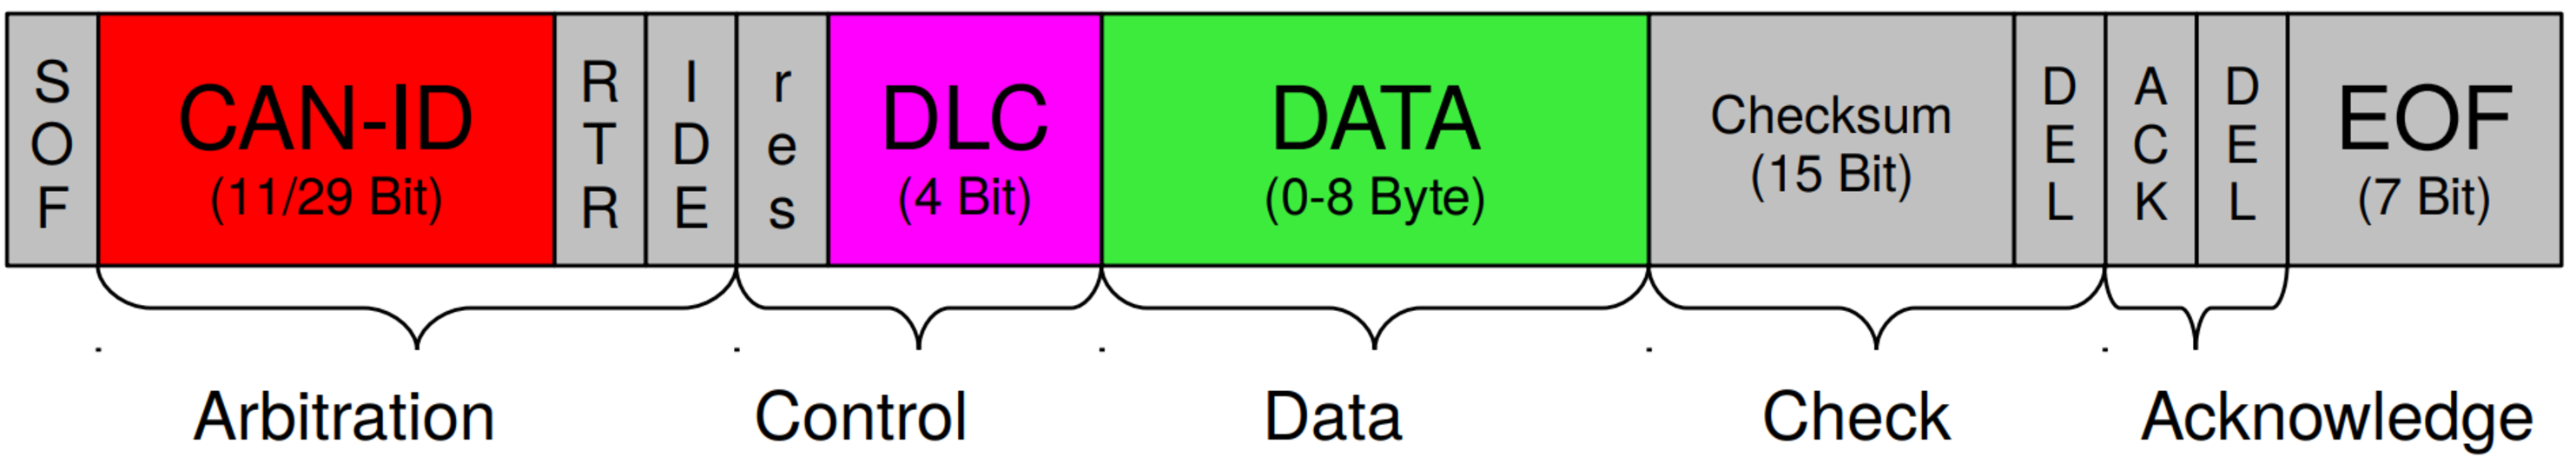
\includegraphics[width=1\textwidth]{images/can_frame.pdf}
 \caption{CAN frame detail \cite{can_frame}}
\end{figure}

 \section{History}
 The Bosch company standardised the CAN in the 1980s as a relatively simple communication protocol which can provide reliable and priority-based communication that is cheap\cite{history}. Another advantage lies in on.board diagnostics, which is widely used for early failure detection through the OBD-II connector. The first version of the standard provided an 11-bit identifier and a load of maximally 8 bytes per message. However, industry development and the increasing number of sensors and control units require a network connection for more defined messages. The response came in 2003 in the form of  ISO 11898-1:2003; the CAN 2.0 enables using an extended 29-bit message identifier with the remaining data load as its predecessor. The most significant change came with the CAN FD in 2015, where FD stands for a flexible data rate. In brief, the flexible data rate means that the data part of the frame is sent at a higher bit rate than the rest of the frame. Because of this change, the data part increased from maximal 8 bytes to 64 bytes\cite{can_fd}. The standard introduced indirect mapping for the data length code to preserve backward compatibility with the older frame format; the result is that not each combination of data bytes length is possible, but a higher payload in a similar time is provided.


 \section{Physical level}
 This section discusses how individual bits are transmitted on the bus. A part of the definition includes transmission speed, bit timing, synchronisation, and signalling levels. The physical layer consists of twisted pair cabling, which improves the shielding from external electromagnetic disturbances. The first wire is CANL, and the second wire is CANH; the logic value on the bus is evaluated as CANH - CANL (differential voltage). Connection is provided by OR logic functionality. Signalling levels are divided into dominant state, termed logic 0, and recessive state, termed logic 1. Each station (node) implements a logical AND.
 
\begin{figure}[htb]
 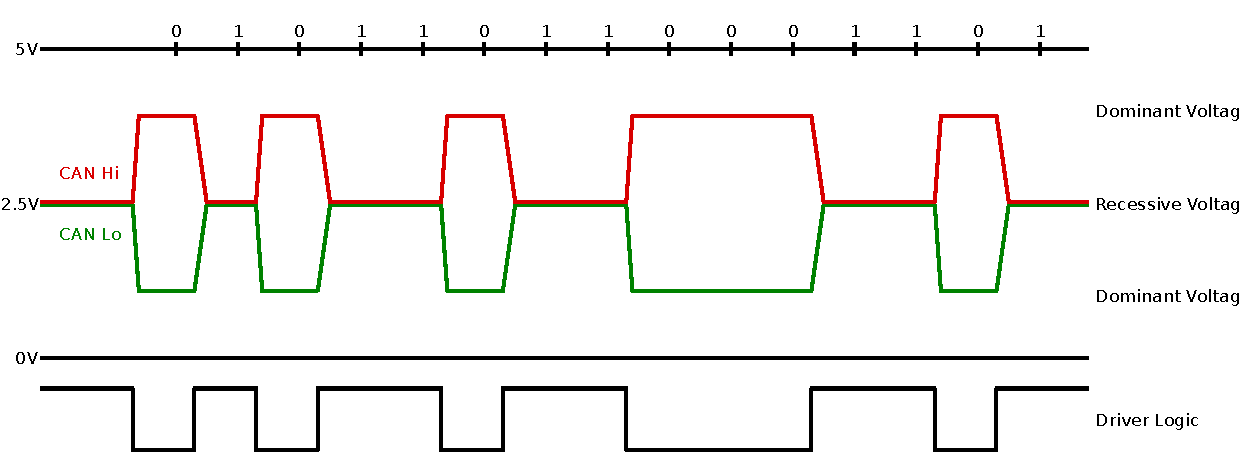
\includegraphics[width=1\textwidth]{images/ISO11898-2.pdf}
 \caption{CAN Bus Physical Layer \cite{can_physical}}
\end{figure}
 
 \section{Logical Link Control}
 Logical Link defines how to inform about overloading of some stations and allow filtering for received frames. The acceptance filter mechanism occurs during a reception and before the incoming frame is stored in the received FIFO. It filters frames based on their frame ID. Consequently, it reduces the load from a single station and decreases demands on its performance because not every message on the bus must be processed from a FIFO buffer. The acceptance filter comprises two bitwise requirements, where at least one needs to be fulfilled; it results in an accepted message. The acceptance mask determines which bits are ignored in comparison to frame ID. Regarding bits which are considered, these are compared with the acceptance code\cite{can_filter}.
 
 \section{Medium access control}
 The main idea is that each station (node) is equal to others during communication - peer to peer and frames are broadcasted. Identification is based on unique frame IDs, independently of specific nodes. Lower ID means higher priority on the bus; the exact principle is described below. In case of an error, the station should retransmit the frame. MAC prevents destructive collisions and defines how long the station will wait for transmission. If the station wants to start communication, it is necessary to detect Idle State on the bus, which means 11 recessive bits - logic 1. The CAN bus runs the CSMA/CR protocol, where CR stands for collision resolution \cite{can-course}. Each station starts to transmit bits from frame IDs and reads the state on the bus simultaneously. Logical 0 as a dominant state always wins against logical 1; if the station sends 1 to the bus and reads 0, it loses the arbitration and immediately stops transmitting. This process determines the node with the lowest ID, which is then allowed to continue transmission. The CAN standard features a mechanism to request a specific frame. The principle is to send zero data length frame with wanted ID and set the RTR bit occurring immediately after frame ID to logic zero. As a response to the RTR frame, required data should arrive.
 
 \section{Bit stuffing}
 The CAN bus does not have a wire for a clock, which means there is no fixed clock. Synchronisation is made on the bit-level during falling and rising edges. The bit stuffing is a mechanism that forces the transceiver to add an opposite bit to 5 identical continuous bits.
  
\begin{figure}[htb]
 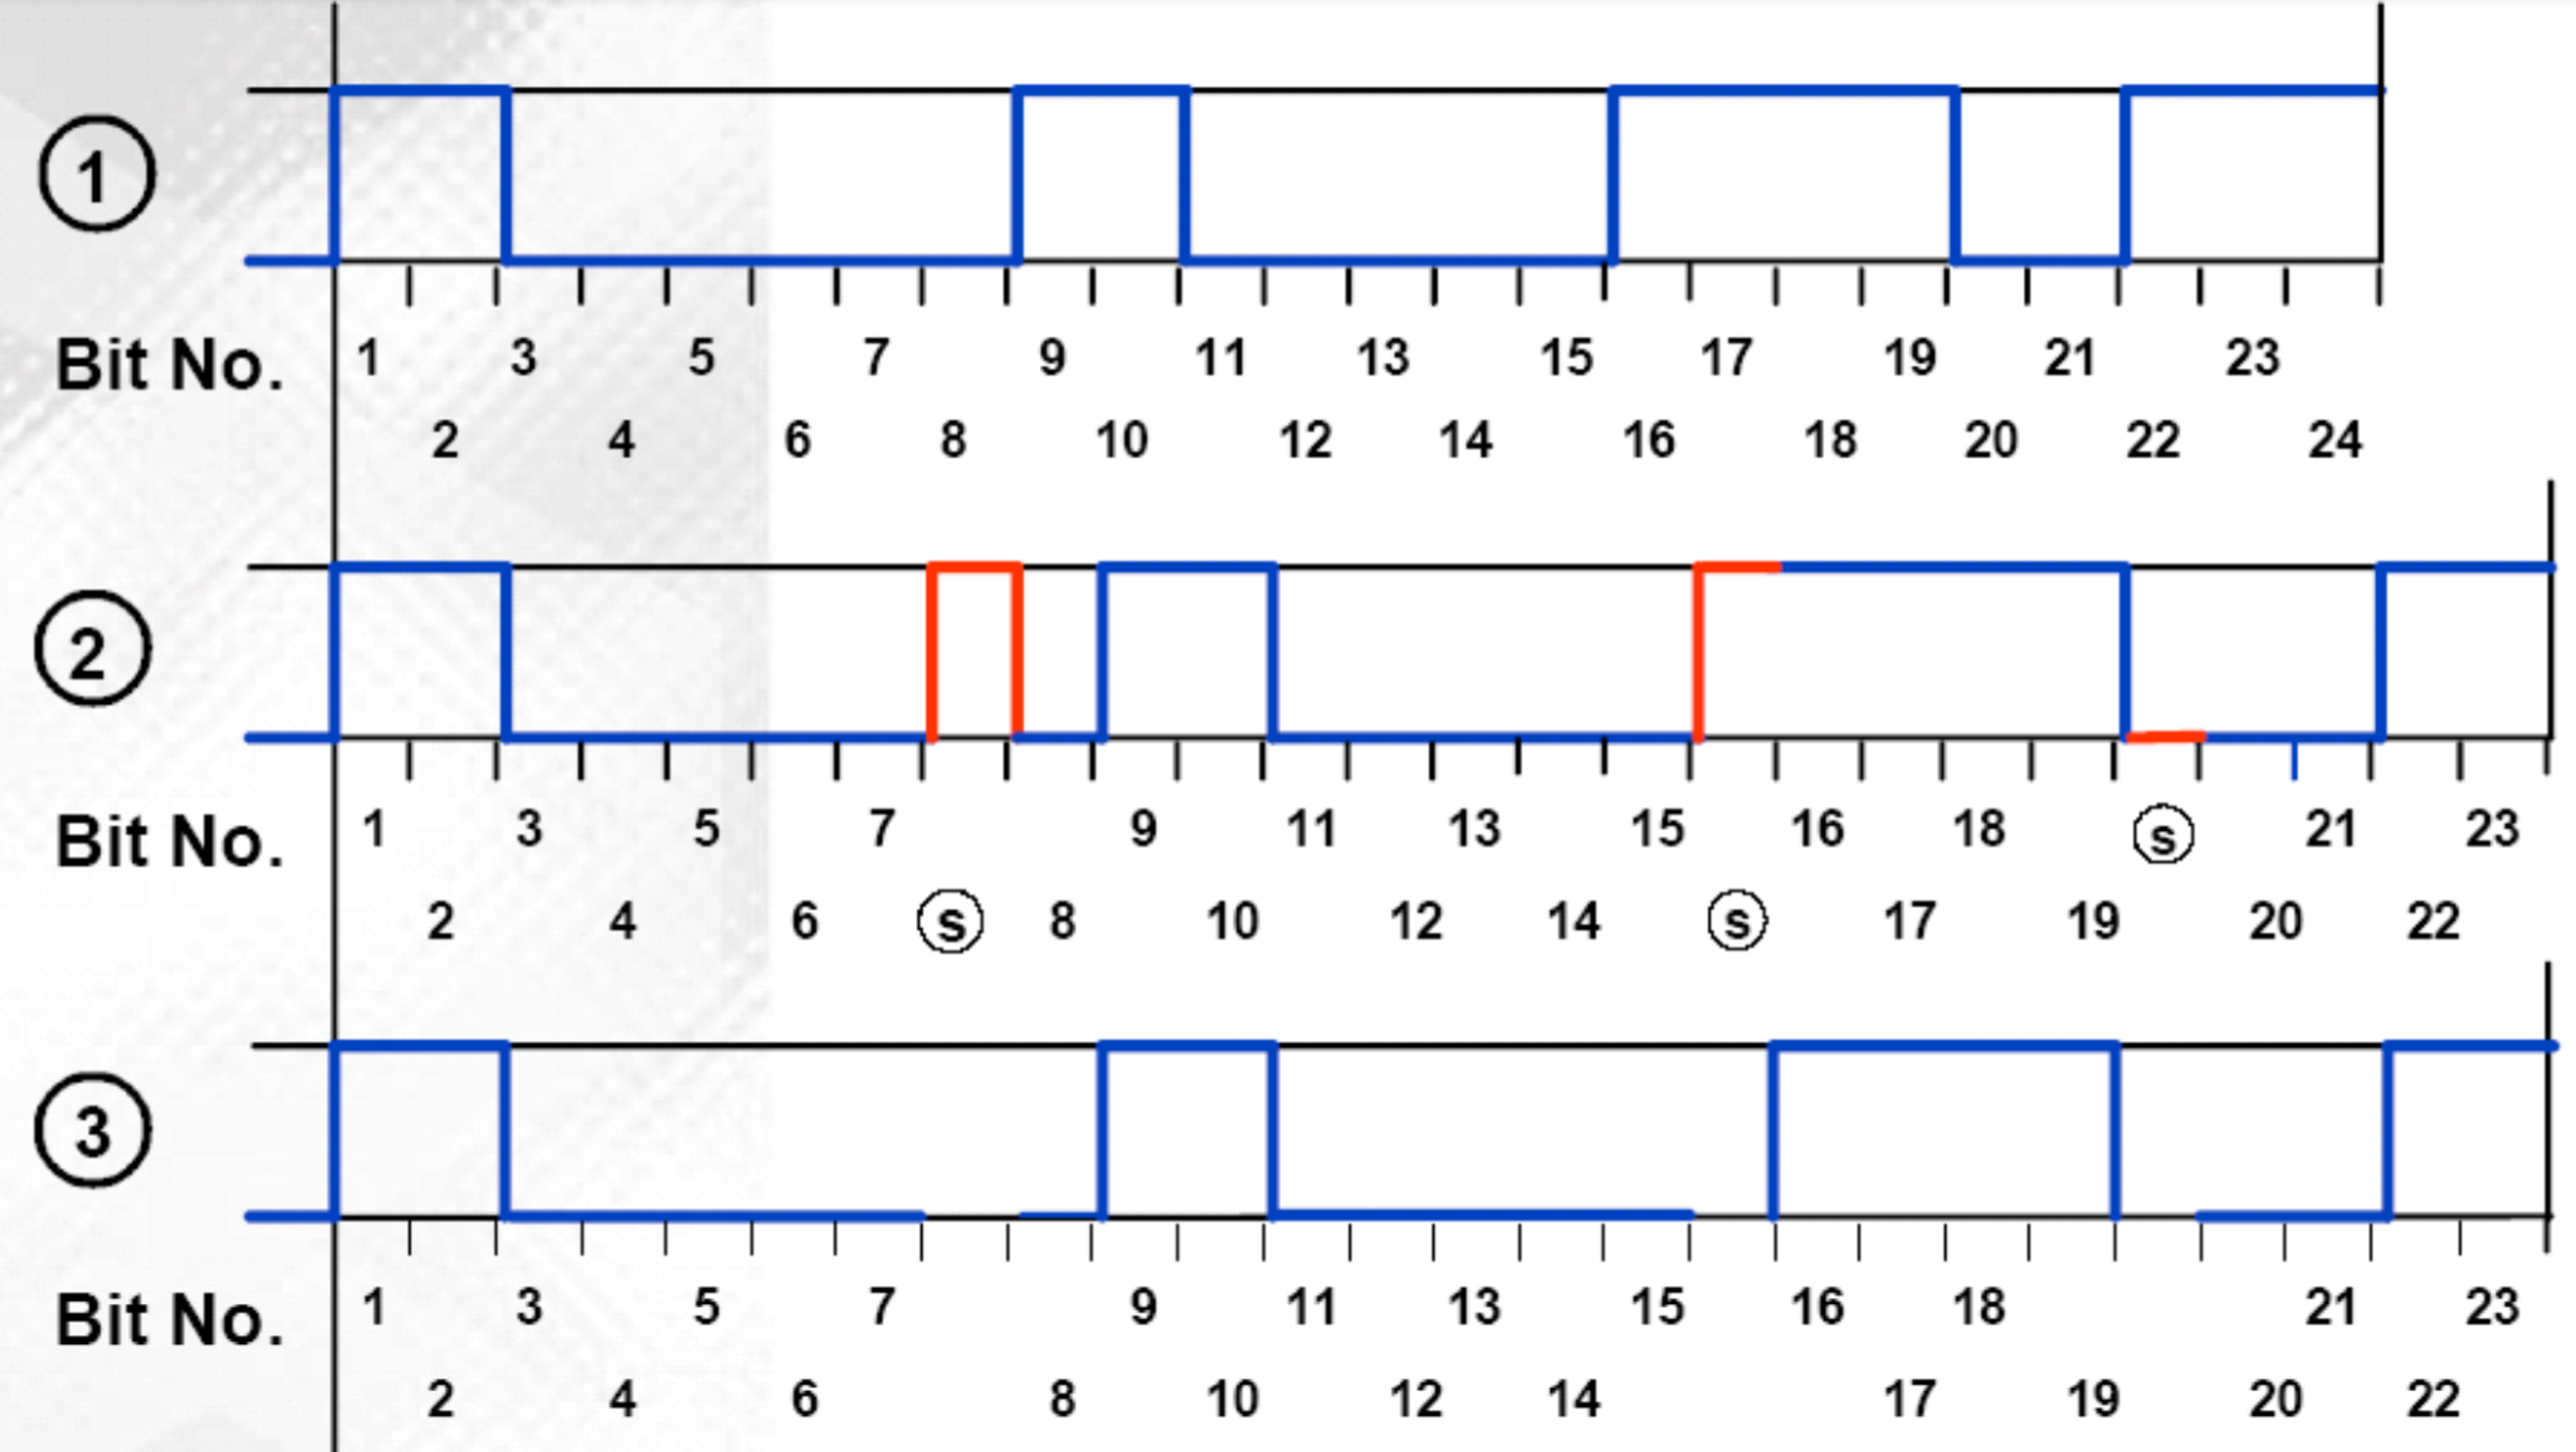
\includegraphics[width=1\textwidth]{images/bitstuffing.pdf}
 \caption{Bit stuffing \cite{can-course}}
\end{figure}
 
 \section{Error Detection}
 On the bus, continuous error detection is performed at every station. Splitting errors into two classes is possible depending on when they occur - during transmission, or during reception. The first controlled rule is to read the same logic state as the station sends. The only exception is a lost arbitration, where another station has a lower ID and therefore wins; this leads to the necessity to stop transmitting by the lost station. During receiving, it is checked whether the mechanism of bit stuffing is respected. After reception of almost the whole frame, CRC is calculated from the data part and compared with CRC in the frame, and it must correspond. At least one other station must confirm the reception of the frame during the ACK bit; otherwise, an Error Frame is sent. When any station notices an Error Frame, the mechanism is that an Error Frame breaks the bit stuffing rule, and then it replies with its Error Frame. It ensures the propagation of error to the whole bus.
 
 \subsection{Error states}
 Error measurement consists of error counters in each station; there is one for transmission and one for reception. When the station notices any errors mentioned above, the corresponding counter increases (0, 1, 8), and these counters are then dynamically modified according to bus communication rules. The most common state during communication is an Error Active State. If one counter exceeds 127, the state is changed to Error Passive State: this is a state where the station generates six ones instead of an Error Frame and cannot influence other stations. The counter can be decremented if another frame is transmitted or received correctly. The Upper bound for any station is 255. Passing leads to a Bus-off State. The station gets wholly disconnected from the bus and cannot affect or read communication until passing several intraframes. Disconnection of the possibly broken station allows the rest of the stations to stabilise. Thus, the minimum for reconnecting to the network is 128 sequences of intraframes (at least 11 ones).
 
 \section{Bit Timing}
 The CAN bus is lacking clock signal shared among the stations. Therefore, there has to be a designed algorithm to keep the communication and frequency synchronised. It requires a stable and robust solution because it should function in 20 years old car. During this time, the system is exposed to vibrations, electromagnetic fields, or degradation of internal oscillators in each station. A transmission of several stations at once can serve as a sample arbitration; this leads to the necessity to keep each bit synchronised. The CAN distinguishes between two types of synchronisations, and both perform on recessive to the dominant edge. The Hard Synchronisation occurs only at the start of the frame (SOF) after the bus is in Idle State. On the other hand, Resynchronisation is executed on every other edge during communication.
 
 \subsection{Bit Composition}
 Each bit is decomposed into smaller pieces, defined as a Time Quantum $T_{q}$, determined by the oscillator. Because of that, a Bit Time is given as a multiplication of a number $N$ and a Time Quantum.
 \begin{equation}
 T_{q} * N = T_{b}
\end{equation}
 For each $T_{q}$ within the bit, it is possible to assign a segment for a certain purpose. The first segment of the bit is always the Synchronisation Segment, and it lasts only 1 $T_{q}$. Here should come the edge of a bit in the optimal case. The following segment is called the Propagation Segment, and it balances a communication delay between the two farthest nodes. The rest is divided into Phase Segment 1 and Phase Segment 2, which define the sample point's exact position, where the sample is evaluated. The PS1, together with the Propagation Segment, can be prolonged; this is the case when the Synchronisation Segment arrives later from the bus. In this case, the bit length is longer by the same number of $T_{q}$s, which takes a delay on the expected vs actual bit start. This mechanism leads to Resynchronisation, and the station is synchronised for the following communication with the same transmitter. The inverse process works if the Synchronisation Segment occurs earlier than expected; the exact $T_{q}$ number must be subtracted from PS2.
 
\begin{figure}[H]
 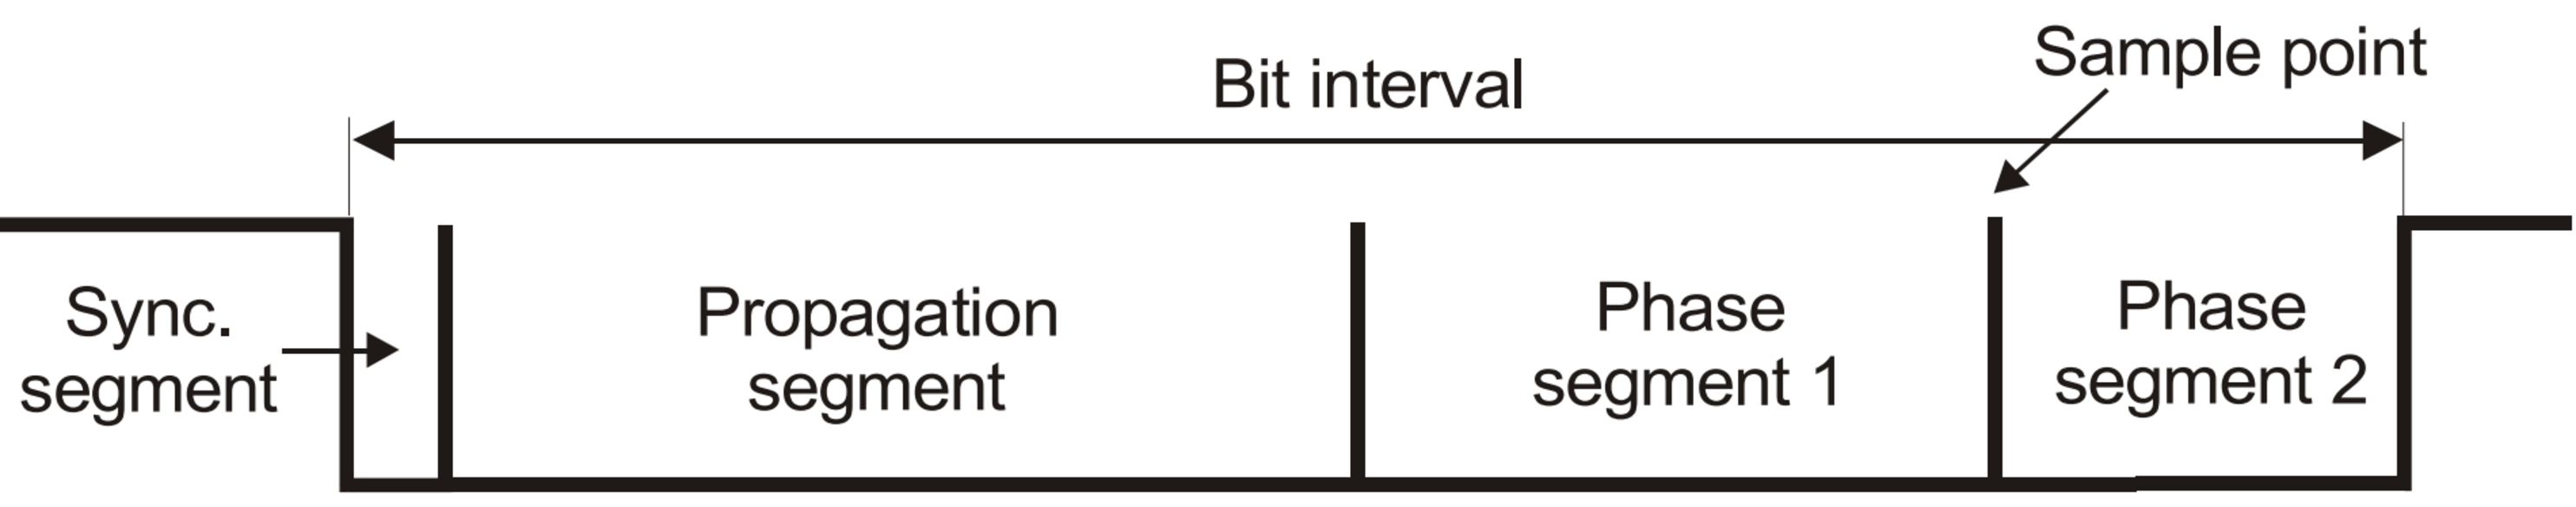
\includegraphics[width=1\textwidth]{images/can-bittiming.pdf}
 \caption{Bit composition \cite{can-course}}
\end{figure}
 
 \subsection{Example}
 For further calculation, it is possible to assume the speed of electric signal propagation as five ns per meter, and one $T_{q}$ is 100 ns. One of the standard distributions is 20 $T_{q}$s for a bit, then 100 * 20 equals 2000 ns; this stands for bitrate 500 of Kbits per second. If the Propagation Segment is chosen to be 10 $T_{q}$ long and the Phase Segment 1 to be 5, the equation is 100 ns * 15  equals 1500 ns per bit. In this instance, the worst case is the need to propagate information in both directions. It results in two times shorter reaction time, meaning 750 ns. The explanation is that the station will transmit a recessive bit; this information needs time to travel to the farthest node. When the signal arrives, it is a valid sequence that the most distant node starts to send the dominant bit simultaneously, and this information needs time to propagate backwards. 

\begin{verbatim}
100 ns * 20 T_q = 2000 ns -> 500 Kbit per second
100 ns * 15 T_q = 750 ns
750 ns % 5 ns/m = 150 m
\end{verbatim}

 This calculation leads to a possible 150 meters cable length in this optimal case. In practice, latencies on both sides for the transmitter, receiver, and other disturbances have to be added. In summary, it is possible to reach half the length of the cable (~75 m) for this case.
 
%%%%%%%%%%%%%%%%%%%%%%%%%%%%%%%%%%%%%%
%%%                                %%%
%%%           CHAPTER 3            %%%
%%%                                %%%
%%%%%%%%%%%%%%%%%%%%%%%%%%%%%%%%%%%%%%
\chapter{ESP32C3 RISC-V microcontroller}
\label{ch:esp32}
 It is a RISC-V single-core microcontroller, an ultra-low-power and highly integrated SoC by Espressif. It means that it is a completely integrated system in a single package. The processing parts, memory and modems are manufactured together. The modems integrated on the chip are Wi-Fi and Bluetooth 5. The next advantage of SoC is a lower amount of necessary space and power consumption.
 For example, several onboard security features include a secure boot and flash encryption with AES-128/256.

\begin{figure}[htb]
 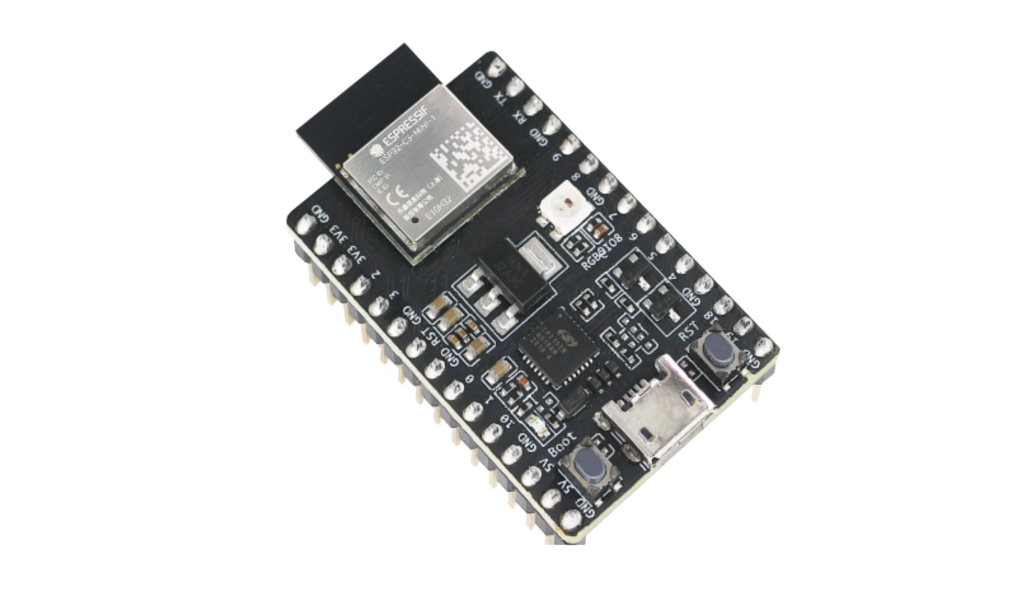
\includegraphics[width=1\textwidth]{images/esp32-c3-devkitm-1-v1.pdf}
 \caption{ESP32-C3 DevKitM-1 version 1 RISC-V \cite{esp32c3-devkit}}
\end{figure}

 \section{ESP32C3 DevKit}
  A development kit has been provided to develop the NuttX driver by the Espressif company. It has module ESP32-C3-MINI-1 with Wi-Fi and Bluetooth 5\cite{esp32-c3-mcu}. The board contains address space divided into 800 KB of internal memory space for instructions, 800 KB of internal memory space for data, 1016 KB of peripheral address space, 8 MB of external memory for instructions, and 8 MB of external memory for data, 480 KB for DMA. Altogether 800 KB of internal memory and up to 16 MB of external memory, and 35 peripherals, including TWAI.

\begin{figure}[htb]
 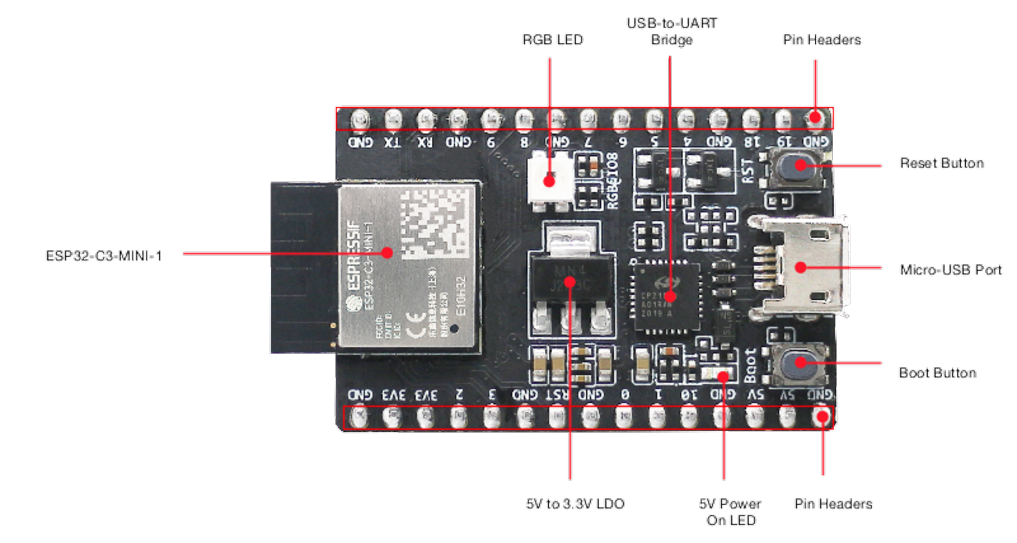
\includegraphics[width=1\textwidth]{images/esp32-c3-devkitm-1-v1-annotated.pdf}
 \caption{ESP32-C3 DevKitM-1 version 1 RISC-V with description\cite{esp32c3-devkit}}
\end{figure}

 \section{Espressif SDK}
  ESP-IDF is an official development framework\cite{esp-idf}; it is prepared for the whole ESP32 SoC family containing several boards. It enables the programming of specific boards, as well as their debugging, and helps make development easier. It can be found as an open-source on GitHub in several versions; more information is provided in the installation section about versions and releases\cite{otrees}.
  
 \subsection{Download ESP-IDF}
 First, it is necessary to download ESP-IDF \cite{esp-idf-guide} - the official development framework for ESP32. It is available at the git repository. Nevertheless, online and offline installers are prepared, and they are very convenient because they solve all the prerequisites and linking problems\cite{esp-idf-intallers}.
 If the development framework is already installed, staying up to date on the newest version is recommended. This series of commands requires to be run every once in a while.
\begin{verbatim}
cd %IDF_PATH%
git pull
git submodule update --init --recursive
\end{verbatim}
 It is also possible to change between stable or release versions.
\begin{verbatim}
git pull
git fetch
git checkout vX.Y.Z
\end{verbatim}
 Finally, finish switching by the same commands as are used for updating.
 
 \subsection{ESP-IDF Hello world}
 After successful installation, it is time to run the first program. This process has good documentation on Espressif websites under the appropriate chip and version selection. Start with running ESP-IDF CMD in the top hierarchy location of installed ESP-IDF in the file system. It should be accessible by running this command.
\begin{verbatim}
cd %IDF_PATH%
\end{verbatim}
Here we can find file export.bat, which temporarily adds all the necessary tools to the environment variables.
The ESP-IDF folder features prepared examples, including $hello\text{-}world$. It can be copied out of the hierarchy with the command $xcopy$.
\begin{verbatim}
xcopy /e /i
      %IDF_PATH%\examples\get-started\hello_world hello_world
\end{verbatim}
Go to the newly created $hello\text{-}world$ folder and run the command, which induces the download of all necessary dependencies and prepares the project to run.
\begin{verbatim}
idf.py set-target esp32c3
\end{verbatim}
For this simple program, nothing else needs to be done, only ascertain which port  a device is using - for example, through device manager - and run.
\begin{verbatim}
idf.py -p PORT flash monitor
\end{verbatim}
Application builds and flashes onto the chip; monitor command shows output on the serial line. An identical working procedure could be applied for a similar example called blink, which should turn the LED on and off. One more example can be recommended and is hidden under the following path.
\begin{verbatim}
cd %IDF_PATH%\examples\wifi\getting_started\softAP
\end{verbatim}
After running this command, it is possible to connect to ESP32 via WIFI, e.g. on a mobile phone.\newline

\quad A potential problem to be careful of – if it is the first program on the board - it is possible that a bootloader is missing - the bootloader and partition tables should be present in a flash\cite{esp-idf-bootloader}. Both corresponding files are located, for example, here on Espressif GitHub. They are marked as NuttX specialised, but they are the same as ESP-IDF's examples are using by default. Then it is enough to run this command with correct paths to binary files.
\begin{verbatim}
esptool.py --chip esp32c3 --port PORT --baud 921600 write_flash
           0x0 bootloader-esp32c3.bin
           0x8000 partition-table-esp32c3.bin
           0x10000 hello_world.bin
\end{verbatim}
The example above flashes $hello\text{-}world$ binary, and on the top of that also loads a new bootloader and partitions tables. Now the board ought to be entirely wiped out and ready to run the selected program. 
 
 \subsection{ESP-IDF TWAI}
 This work’s target is CAN bus development, so it is reasonable to find and try the TWAI examples to ascertain whether they are running correctly.
\begin{verbatim}
cd %IDF_PATH%\examples\peripherals\twai
\end{verbatim}
Several projects are at disposal in this directory.  However, these examples require additional hardware to be run. For two of them, it is sufficient to have a small jumper for the connection of two neighbouring pins. The third example requires another board, and each extra board requires its external CAN transceiver – therefore, this example will not be tested.
TWAI self-test has to be configured the same way as all examples before. It is recommended to check correct pin settings in:
\begin{verbatim}
idf.py menuconfig
\end{verbatim}
It should be configured to pins number 2 for transmitting and number 3 for receiving. These two pins have to be connected to valid testing results.
\begin{verbatim}
idf.py -p PORT flash monitor
\end{verbatim}
An identical configuration is valid for the second example, TWAI alert and recovery. It tests the ability to recognise an error on the bus (cause the bus off state) and reconnect the device again. Both tests mentioned above are correctly concluded if written on the console - driver uninstalled; it means that the testing sequence ends successfully.

 \section{RISC-V architecture}
  Firstly, it is necessary to explain the term ISA; Instruction Set Architecture is a model of registers and code instructions\cite{risc-v}. Each architecture, such as Intel x86 or ARM, has its ISA. This abstract model set is licensed; the manufacturer must pay to produce hardware based on these ISAs. RISC-V has an open-source license and was developed and maintained by specialists in computer architecture. It is possible to have a 32-bit or 64-bit system. RISC-V is RISC architecture equivalent to ARM.

%%%%%%%%%%%%%%%%%%%%%%%%%%%%%%%%%%%%%%
%%%                                %%%
%%%           CHAPTER 4            %%%
%%%                                %%%
%%%%%%%%%%%%%%%%%%%%%%%%%%%%%%%%%%%%%%
\chapter{NuttX RTOS}
\label{ch:nuttx}
 NuttX is a real-time operating system targeting an embedded environment. Its main philosophy is to keep a small footprint but provide broad standard compliance for sample POSIX and ANSI standards. NuttX is highly configurable, which means that a project could retain only the desired components. The small footprint is accomplished by compiling and including only the features used into an executable file and many other mechanisms. In other words, each peripheral or any other part can be added or removed from the build before compilation due to its modularity\cite{nuttx_about}. Kconfig system stands for configuration purposes, similarly to Linux. The building system used after configuration from Kconfig is GNU makefiles. Development is currently run under The Apache Software Foundation and Apache License 2.0. NuttX comes with RTOS features such as exceptional schedule management for sharing resources - it is fully preemptive. It has task priorities with the possibility of priority inheritance or Symmetric Multi-Processing, and for multithreading semaphores, pthreads or mutexes. RTOS determines that the system must pass multiple strict conditions, and each critical event has its defined maximum realisable time.

 \section{NuttX advantages and comparison}
  The NuttX can be used in embedded systems due to its miniature footprint, and therefore it is optimal for low-cost microcontrollers with a small FLASH and RAM. Nevertheless, NuttX is also convenient for modern microcontrollers, where the size of the FLASH is counted in megabytes because more features can be applied. It is possible to mention a configurable protected build with MPU providing protected memory access. MPU creates kernel and user mode access, where kernel-mode remains unlimited, but user-mode can have limited register access or machine instructions\cite{nuttx_protected}. \newline
  
  \quad Another advantage lies in an approach to the file system because it keeps comparable to more extensive systems such as Linux. The file system boots in a pseudo root file system, but there is a possibility of mountable volumes enabling utilising the same techniques that are usually used on Linux via the $mount()$ function. NuttX is not dependent on any file system and implements functions such as open, close, read, write or IOCTL calls. Furthermore, even small application has a device driver supporting structure. The compatibility leads to possible mitigation of code written and validated on Linux with few or no adjustments to run on NuttX.  \newline
  
  \quad A project with a similar aim is Zephyr RTOS which targets embedded environments. Zephyr originates from the Wind River Company and has good documentation\cite{zephyr}. Another example of such a project may be Mbed OS, commonly used in embedded applications. It has an RTOS core, provides clean API to C++ applications, and is more straightforward\cite{mbed}.

 \section{Configuration}
  A complete list of commands explained in detail is available in the NuttX configuration\cite{nuttx_start}. It will only be described briefly hereinafter. An already prepared configuration could simplify the first steps of configuring NuttX because it sets the basic settings, which may be hardware-dependent. For this purpose, a script called configure.sh is prepared in the $tools$ directory. This script needs an argument composed of a board name - target hardware - connected by a colon with a configuration name.
\begin{verbatim}
./tools/configure.sh esp32c3-devkit:nsh
\end{verbatim}
 NSH configuration fits the best because it leads to a simple application with NuttShell using serial standard input and output. It also helps in terms of the testing purpose for the first run on a particular device.  \newline
  
  \quad Manual configuration is done with Kconfig language, which is also used in Linux. It is organised as a collection of configurable options in a tree structure, where dependencies are considered. As a result, they affect the visibility of individual records. Logical units are stacked and follow the exact syntax. Final configuration windows consist of several Kconfig files around a system\cite{kconfig}.
\begin{verbatim}
make menuconfig
\end{verbatim}
 NuttX can export a newly created configuration in two ways. The first automated way makes the .config file during the compilation. It contains all configurable options and their values; it stores all information because some default values can change during NuttX development. The second way is calling the command, which produces a compressed configuration file named defconfig, including only changed parameters from the default value.
\begin{verbatim}
make savedefconfig
\end{verbatim}
 All configuration files, called by the $configure.sh$ script, are in the form of the compressed file as defconfig.

 \section{Directory Structure}
 The file system hierarchy is similar to Linux,  it features the description of the necessary folders for further work. The first and the most relevant folder visible in the NuttX root directory is called  $arch$ and contains architecture-specific code. It is logically divided by the target architecture. For this thesis, $arch/risc\text{-}v$ and then $arch/risc\text{-}v/src/esp32c3$ directories are the appropriate way to move. The essential parts of the drivers or chip-specific register definitions are defined here. It is also the location of Kconfig responsible for setting parameters for specific peripheral or functionality of the target hardware. Finally, this section also features a makefile which includes configured peripherals or functions into a build. Back in the root NuttX directory, there is the $boards$ folder with logic supporting individual boards. According to the system requirements, the driver initialisation and bring-up logics are for the ESP32C3-devkit on the path $boards/risc\text{-}v/esp32c3/esp32c3\text{-}devkit$. This significant folder includes adding above mention logic to a compilation by modifying the corresponding makefiles and calling the setup function prepared for a particular driver. The rule is valid for source files, but one more directory called $configs$ is prepared on this path, and there are several configurations for setting up NuttX from scratch.  \newline
  
  \quad Furthermore, the folder accessible from the top of the directory structure is $driver$. This section incorporates general NuttX drivers that are not hardware-dependent, including the upper half of the CAN driver. The final item mentioned here is the $tools$ directory, including a configuration script or a script for checking the coding style.

 \section{Basic work with RTOS}
 The NuttX follows POSIX standard, which means that NuttX supports pthreads. Each task is running in a container called process, which consists of a thread. Basically, when a task is started, it runs its own thread with default priority 100. An example of creating a new thread follows.
\begin{verbatim}
pthread_t thread;
pthread_create(&thread, NULL, thread_func, NULL);
\end{verbatim}
 This sequence creates a thread with a default priority, and the thread runs a function named $thread\text{-}func$. The priority can be changed while the thread is running using the following command.
\begin{verbatim}
pthread_setschedprio(pthread_self(), 110);
\end{verbatim}
 Threads with different priorities can be used for peripheral priority boost. This topic is discussed more in detail in the Testing part of this thesis.
 
 \section{CAN Support}
 CAN has the weal support in the NuttX RTOS. It distinguishes between Character Device Drivers and Specialized Device Drivers. CAN as a character device driver provides only low-level support for communication between stations and offers an approach as a device in the $/dev$ directory. The driver is logically split into two parts. The upper-level general driver provides software FIFO for reception and transmission, API for the user-space applications, and the lower-level driver functions, which the architecture-specific part of the driver must implement. It connects to the low-level driver via callbacks and provides functions to user-space applications. By contrast, the lower-level driver, which is hardware-dependent, provides direct communication with the CAN IP core. Direct communication means initial configuration, working with hardware reception FIFO, transmission FIFO or transmission buffer, depending on hardware design. Another point of view is offered by SocketCAN because it has an approach as the network device which implements a network stack\cite{can_subsystem}. The next difference is that the user-space application is connected via a Socket Layer. This approach  provides benefits in the possible access of multiple applications to one CAN device simultaneously.
 
 \begin{figure}[htb]
 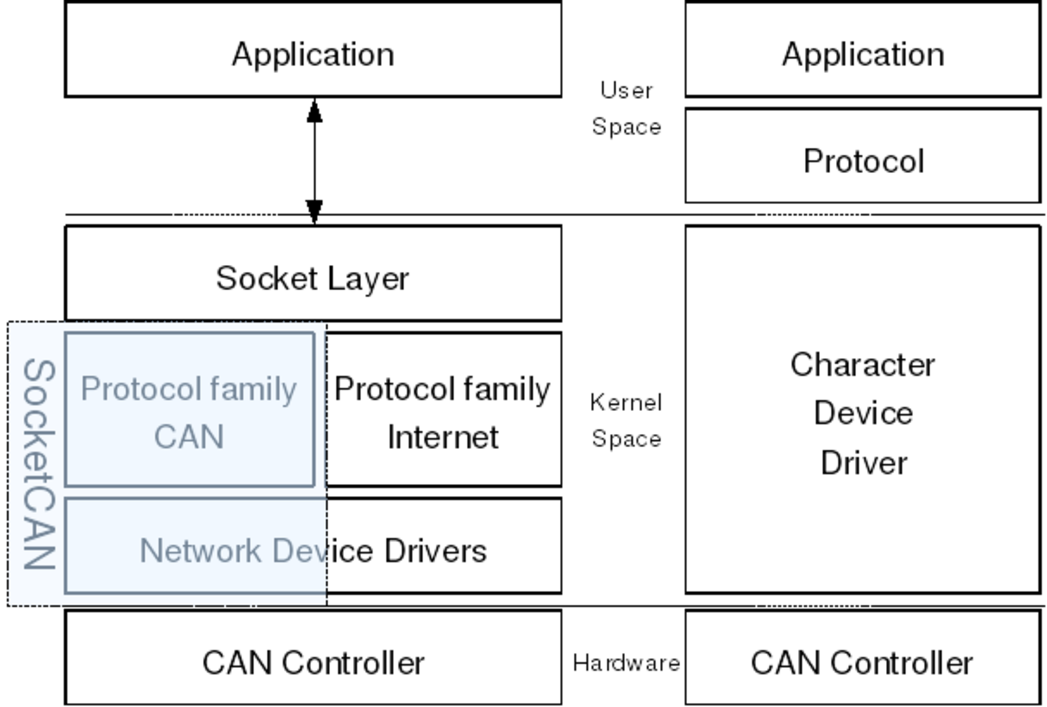
\includegraphics[width=1\textwidth]{images/Socketcan_official.pdf}
 \caption{Driver layout \cite{socketcan}}
 \end{figure}
 
 \section{ESP32-C3 Support}
 The NuttX has already integrated a vast amount of functionality to support the ESP32-C3 board by Espressif. There is prepared a toolchain for compilation or debugging by SiFive\cite{sifive}. It creates an ELF file that must be processed by esptool.py to the ESP32-C3 compatible image and then flashed to the chip. NuttX uses the same bootloader and partition tables for its run delivered with ESP-IDF SDK. The advantage is that this process of uploading bootloader and partition tables can only be done on the first upload; afterwards, only an image file is needed. There is only the ESP32-C3 DevKit board at the time of writing. However, most of the periphery is accessible and is easily and quickly configurable. Easy access is reasonable because several working model configurations for different peripherals are saved in defconfigs. The same applies to application examples in the apps repository that are prepared. The most straightforward is to use the NSH configuration and connect to the serial link via micro-USB or via Tx and Rx pins to use bidirectional communication with the NuttX shell.
 
%%%%%%%%%%%%%%%%%%%%%%%%%%%%%%%%%%%%%%
%%%                                %%%
%%%           CHAPTER 5            %%%
%%%                                %%%
%%%%%%%%%%%%%%%%%%%%%%%%%%%%%%%%%%%%%%
\chapter{Development in NuttX on ESP32-C3}
\label{ch:nuttx-on-esp32}
 Using the Linux operating system during NuttX development is not the only option, but it is the most natural environment. In the case of this thesis, WSL 2 with Ubuntu-20.04 functioned appropriately. ESP-IDF and NuttX feature many build-in examples that can be run to get familiar with the board and with the operating system for embedded devices. Both projects are open-source, and the code is available on GitHub. This chapter illustrates the optimal workflow during contribution to NuttX, and the requirements are explained.

 \section{Start of Cooperation with Espressif Team}
  On the second of November, a meeting took place with Espressif and NuttX RTOS developers on university premises. Firstly, representatives gave a presentation about their companies, and then the projects they were working on were introduced. The second part of the meeting on Karlovo Namesti in CTU FEE discussed future possibilities of collaboration and the goals of this thesis. Espressif had already provided two ESP32-C3 boards several weeks prior to their arrival, so it was possible to get familiar and test some examples. The last part involved something of a workshop, where problematic parts were  consulted together directly at the computer. The consultation included the possibility of debugging on ESP32C3 and some compilation problems with the NuttX example. As a result of the meeting, more ESP32C-C3 RISC-V boards and control register definitions were provided, which served as a necessary element for further development.

 \section{NuttX License}
  NuttX’s long-term philosophy is to be an open-source project under no restrictive and copyleft license. The project has been developed for long time under the BSD license, mainly under the BSD 3 and 4 clauses\cite{license_bsd}. The BSD is not considered a copyleft. It means that anybody has a right to use, modify and share the code from projects with this license. Moreover, a modified source code, thanks to the relaxed rules, is not required to be open-source and does not forbid sub-licensing. The actual licence used in the NuttX is Apache 2.0 License, which is also a permissive license\cite{license_apache}. It is compatible with the formerly used BSD license and was initially very similar to Apache 1.0. Subsequently, Apache 2.0 separated itself from BSD in the relaxation of conditions and now directly determines the rules of patenting the code, which results from the code under the Apache license. It adds the necessity to list modification notes. Another difference is the advantage of using arbitrary files by other projects without changing any word in the headers. All the work resulting from this thesis is published under the Apache 2.0 license. 

 \section{Coding style}
 For developers wanting to contribute to a project of such a size, coding style must be determined. NuttX has its own strict rules for coding style, and they are different from the style used, for example, in Linux or QEMU, which both use a highly similar coding style.  NuttX source tree includes scripts inside the  $/tool$ directory, which can check most problems with written code according to the official rules. The component that checks the file is the $nxstyle$ program, but there also exists a program called $checkpatch$ ”: it is a universal tool because it can check whole patches. Common mistake encountered were incorrect padding, too long lines, or the necessity for the exact style of comments in the code, which differ between line comments and multiline comments. A simple example of the coding style with the if condition is as follows:
\begin{verbatim}
#ifdef CONFIG_ESP32C3_TWAI0
  if (port == 0)
    {
      /* Enable power to the TWAI module and
       * Enable clocking to the TWAI module
       */

      modifyreg32(SYSTEM_PERIP_RST_EN0_REG, 0,
                  SYSTEM_TWAI_RST_M);
      modifyreg32(SYSTEM_PERIP_CLK_EN0_REG,
                  SYSTEM_TWAI_CLK_EN_M, 0);
  }
#endif
\end{verbatim}
Here is an example of calling the script for a newly developed driver.
\begin{verbatim}
./nxstyle -v 1 ../arch/risc-v/src/esp32c3/esp32c3_twai.c
\end{verbatim}
or
\begin{verbatim}
./checkpatch.sh -f ../arch/risc-v/src/esp32c3/esp32c3_twai.c
\end{verbatim}
Empty output means that most mistakes are solved, but something may be found manually during a pull request. For example, padding of function parameters that do not fit into one line length has to start in the same position as the first parameter of the line above, but the script will not find this problem; an example follows.
\begin{verbatim}
  esp32c3twai_set_acc_filter(TWAI_ACCEPTANCE_CODE,
                             TWAI_ACCEPTANCE_MASK, true);
\end{verbatim}

 \section{Related work}
 Prior to writing the driver, it is reasonable to analyse the related work, which would show the right approach to future development. ESP-SDK has a functional driver with working examples enabling data transfer; it is an essential source of knowledge about the proper mechanism and approach to a CAN IP core on the ESP32-C3 board. This implementation should correspond to the official technical reference manual provided by Espressif\cite{esp32c3-trm}. Another one from the interesting sources is LinCAN, written for Linux and capable of supporting RT-Linux, written by Pavel Pisa. LinCAN is appropriate for this thesis because it includes Philips SJA1000 support and has solved the problem of bus timing well. Another elemental source must be found in NuttX RTOS; it contains many implementations of the hardware-dependent side of the driver. After a discussion with the thesis supervisor, the arm-based board named lpc17\text{-}40 was selected. This board supports CAN and includes model driver implementation under NuttX RTOS. 

 \subsection{ESP-IDF TWAI}
 ESP-IDF provides a functional implementation of the TWAI driver on the ESP32-C3 board. The driver is divided into three layers; the lowest layer is hardware-dependent for the ESP32-C3 microcontroller. The control registers of the TWAI IP core are in the memory-mapped peripheral (I/O) region, and the driver uses a technique of accurately mapped structure, where each bit corresponds to the register layout. It is a different approach from the one intended for use in the newly developing NuttX driver. However, it shows set values and can be double-checked against the documentation to verify whether everything corresponds. Among other available information, it can be discovered that there are combinations of modes for sending the messages, parsing received messages and vice versa, and finally, bus timing settings. It is necessary to consider that the ESP32-C3 technical reference manual is still in a preliminary state. The middle HAL layer is common for more ESP32 family microcontrollers and composes the driver handling into a logical block as the initialisation part. Here is a well readable sequence of commands recommended by Espressif for control registers. For example, we can mention the initialisation part, which firstly sets a reset state and reset error counters. The last part of the driver provides user-space public functions for using the TWAI peripheral. This includes the functions for receiving and sending messages.
 
 \subsection{LinCAN}
 The LinCAN driver is one of the first attempts to unify the Linux kernel CAN drivers subsystem for more vendor interfaces\cite{lincan}. It has started to be developed and designed before a SocketCAN implementation by Volkswagen Pengutronix. The LinCAN is based on a character driver; it registers a character device. It implements multiple FIFO queues for different priorities of sent messages. The LinCAN supports SJA1000 and Intel CAN controllers. \newline 

 \quad LinCAN provides a relatively well-elaborated mechanism to compute bit timing according to the parameters of the specific controller\cite{lincan-code}. It calculates the Time Quanta, Synchronisation Segment, TS1 and TS2 for different controllers. SocketCAN later adopted the mechanism for all Linux supported controllers. \newline

 \quad SJA1000 is a simple CAN controller developed by Philips (NXP)\cite{sja-1000}. It provides a single TX buffer for sending the message. There is a FIFO queue based on the byte granularity for the input, so incoming messages are recorded into this FIFO. The capacity of FIFO is relatively small (64 bytes). It can be optimally distributed between short or long messages.

 \subsection{lpc17\text{-}40 CAN}
 lpc17\text{-}40 is an ARM architecture based microcontroller with an exemplary implementation of CAN driver under NuttX RTOS. This microcontroller has two CAN cores, unlike ESP32-C3, which has only one. Nevertheless, it is reasonable praxis to write the code as general as possible so that it will take into consideration the future possible addition of more cores in the ESP32 SoC family. Therefore, this microcontroller is an excellent candidate to be the NuttX side model for the newly developed driver. The structure of the driver is comparable to the developed new driver, so that more information can be found in the driver development section.  The CAN driver for stm32 is very similar, but with even more functionality provided ; for example, this driver implements IOCTL calls.
 
 \section{Debugging}
 During development, it is essential to have tools and techniques to debug the code, to be able to trace a bug and repair it. ESP32-C3 does not have visual output onboard, such as an LCD or several LEDs. Therefore, most of the debugging time is concentrated on the serial line. Here are some options which a programmer has at their disposal, such as print debugging and debugging using JTAG. A problem with writing more complex code, for example, a driver, has to be implemented an extensive part of the driver for basic functionality like receiving or transmitting.  
 
 \subsection{Debug prints}
 NuttX has a wide scale of debug features, and debug options are divided into three levels. It is hierarchically based, which means that the next debug level could be enabled only after the previous one. When general debug output is enabled, it is possible to choose which peripherals will have the right to write to the console device, for example, the NuttShell in the serial console. The CAN peripheral has defined its own debug functions, which prints the intended message and adds the function’s name that triggered this print. The top-level is Error output in the CAN environment used by function canerr—example of usage.
\begin{verbatim}
canerr("ERROR: Unsupported port: %d\n", port);
\end{verbatim}
 It continues with Warnings level.
\begin{verbatim}
canwarn("Remote request not implemented\n");
\end{verbatim}
 The last level is Informational Debug Output; most of the information is hidden here, and it is possible to use it to check the correct behaviour of the driver.
\begin{verbatim}
caninfo("%08" PRIx32 "<-%08" PRIx32 "\n", addr, value);
\end{verbatim}
 One of the techniques is to print the address and the content of a particular register if it is written to it or read from it. In general, Debug prints affect exact timing and, in extreme cases, also the behaviour. A partial solution can be offered by a possibility to create a new thread, which will periodically read and print the content of every critical register. The thread might have lower priority, and it should not influence the driver workflow. Then the content of the registers can be analysed  and possibly find a miss-configuration or other error.
 
 \section{CAN Configuration on NuttX}
 NuttX is a highly modular system and emphasises a small footprint. These rules are also valid for CAN driver support. It has several configuration possibilities, and each affects the exact size of the can message or code, which goes to compilation. The default configuration corresponds to standard CAN 2.0A, where standard frames are used with 11 bits ID. The header includes an identifier in $uint16\text{-}t$ type, 4 bits for data length code, and a one-bit specifies remote request. The data part consists of an 8 bytes buffer because the data length code is a value between 0 - 8. In this case $sizeof()$ function returns a size of 3 plus 8 bytes for the CAN message. If configuration enables CAN extended IDs (CAN 2.0B), the driver is required to be able to store 29-bit identifiers; this leads to the necessity to use the $uint32\text{-}t$ type. This configuration results in a size of 5 plus 8 bytes of the CAN message. The most remarkable change comes with enabling CAN FD because the data buffer has to be lengthened to 64 bytes, and the header needs three state bits in addition. Combined with extended IDs, it gives 6 bytes in the header and 64 bytes in the data part. The difference between the lowest message size (11 bytes) and the highest configurable size (70 bytes) is visible. The NuttX uses an ingenious macro system for this functionality, which enables keeping the image as small as possible. The demonstrated rules are also valid for the code itself; therefore, a maximum of the unused code is delimited from the build.

 \section{API for the lower half of the character driver}
 The backbone connection between the upper and lower half of the driver is the structure called $can\text{-}dev\text{-}s$. It contains several state information or other data required by the upper half driver, but the most important for the lower half driver developer are $struct can\text{-}ops\text{-}s *cd\text{-}ops;$ and $void *cd\text{-}priv;$ structures. In terms of interfacing, the $cd\text{-}ops$ structure is fixed, as it contains several central functions that the lower half driver must support. Here is the list of these functions; a more detailed description is in the implementation part, where each function must be implemented.
\begin{verbatim}
dev_reset(dev)
dev_setup(dev)
dev_shutdown(dev)
dev_txint(dev,enable)
dev_rxint(dev,enable)
dev_ioctl(dev,cmd,arg)
dev_remoterequest(dev,id)
dev_send(dev,m)
dev_txready(dev)
dev_txempty(dev))
\end{verbatim}
The second important structure is in $cd\text{-}priv$ – it contains the whole state and essential information for the lower half driver. By definition, void* is without a fixed structure, and how this structure will be defined is entirely determined by the lower half. The structures above provide API for the upper half driver. Three functions are propagated in the opposite direction. The first, a function $can\text{-}register$, is called after the CAN initialisation part, and this function takes the parameter of the newly created $can\text{-}dev\text{-}s$. The second function, $can\text{-}receive$, is required after reading a message from the HW FIFO. This function's purpose is to copy the message to the SW FIFO. The last one, $can\text{-}txdone$, is called when the CAN controller contains the queueing of outgoing messages feature. This functionality is not compatible with ESP32-C3, and it is therefore not necessary to use that last function in this project.


%%%%%%%%%%%%%%%%%%%%%%%%%%%%%%%%%%%%%%
%%%                                %%%
%%%           CHAPTER 6            %%%
%%%                                %%%
%%%%%%%%%%%%%%%%%%%%%%%%%%%%%%%%%%%%%%
 \chapter{Driver development}
\label{ch:driver}
  This chapter is the central component in the practical part of this thesis. It describes the sequential process of developing the TWAI (CAN) driver for the NuttX operation system. The work started by obtaining controller register definitions provided by Espressif. The next step was to integrate the new driver into the whole NuttX system. It comprised the correct configuration in the Makefile structure and added a driver init call to the board bring-up section. A part of integration was also understanding the Kconfig language to provide users with several possible TWAI (CAN) communication parameter configurations. And the final stage was the driver development itself.
 
 \section{Controller registers}
 In terms of the controller registers, the definitions were not ready at the time; therefore, manual interaction was needed from the Espressif side. Fortunately, the ESP32-C3 controller register definitions were generated immediately from a similar ESP32-S2 chip's CSV and necessary changes were made. The suggested source of register level documentation is in the Technical Reference Manual in the TWAI registers section, where all registers are described in their entirety. During the driver development process, it was recommended to double-check the layout of the bits, but no problem was detected. The resulting header file had to conform to formatting NuttX conventions like all other files. This code is architecture-specific and belongs to the hardware folder specified for register definitions. Register position is set by $\#define$ in the position of the base address chosen for the TWAI peripheral plus register offset. Example for TWAI status register and its definition:
\begin{verbatim}
#define TWAI_STATUS_REG (DR_REG_TWAI_BASE + 0x8)
\end{verbatim}
 A Group of several macros with the same structure also define individual fields within the specific registers. It could be shown as an example on the register field for checking whether the packet prepared in data registers is complete. The first definition helps one-bit fields to decide the $if condition$ for yes-no state recognition without any additional shifting.
\begin{verbatim}
#define TWAI_MISS_ST (BIT(8))
\end{verbatim}
 The following $\#define$ sets the same register field's maximal value in the correct place within the register.
\begin{verbatim}
#define TWAI_MISS_ST_M (TWAI_MISS_ST_V << TWAI_MISS_ST_S)
\end{verbatim}
 The subsequent line defines maximal value.
\begin{verbatim}
#define TWAI_MISS_ST_V 0x00000001
\end{verbatim}
 The last  line defines the shift within the register.
\begin{verbatim}
#define TWAI_MISS_ST_S 8
\end{verbatim}

 \section{Driver Integration}
 Before the driver itself could be written, the whole structure for correct inclusion into the build must be added. This directs attention to NuttX boards section, where  the function $esp32c3\text{-}bringup()$ is located. If CAN is enabled, the entry point to initialise the whole peripheral is there. Function $esp32c3\text{-}twai\text{-}setup();$ is called from the $bring up$ section and tries to initialise the TWAI driver and register it. Makefile includes the file $esp32c3\text{-}twai.c$ into build with its function $esp32c3\text{-}twai\text{-}setup$. The condition below is only fulfilled if CAN is enabled in the configuration.
\begin{verbatim}
ifeq ($(CONFIG_CAN),y)
  CSRCS += esp32c3_twai.c
endif
\end{verbatim}
 The $setup$ function connects the upper and lower driver and their data. The initialisation of TWAI is the first function called from the lower driver, and it returns $can\text{-}dev\text{-}s$ containing the necessary functions implemented inside. The structure is passed to the upper driver in the $can\text{-}register$ function. Because ESP32-C3 has only a single TWAI core, it is automatically registered as can0 (twai0).

 \section{TWAI driver options}
 Kconfig system is used to set the parameters, as in the whole NuttX RTOS. The path is:
\begin{verbatim}
System Type -> ESP32-C3 Peripheral Support -> TWAI (CAN) 0
\end{verbatim}
 It has to be enabled, then occurs settings:
\begin{verbatim}
System Type -> ESP32-C3 Peripheral Support ->
-> TWAI driver options
\end{verbatim}
 The first two options are for TX and RX pins. It can be an arbitrary GPIO pin, according to Espressif's datasheet. The idea is to provide default values, wherever necessary, to have an immediately runnable configuration after the TWAI driver is enabled. The following four parameters belong to bus timing. More than one approach is possible in this instance. The user can be given complete control over all the parameters of bus timing. However, it is not trivial to set these parameters correctly, so at least some checks can be added in order to ensure that the parameters are in suitable intervals and meaningful. A similar approach as in Linux was chosen here in this project. It means that the user is asked only for the specification of bitrate and a sample point ratio. It is expected to have the sample point in an interval of 1 - 100, and the algorithm calculates all the necessary parameters. The other two bus timing parameters are SJW, which limits the number of Time Quanta corrections during bit Resynchronisation, and Sampling, which decides whether the bus is sampled three times. The last parameter, which was recently added and is not even in the mainline\cite{nuttx-mainline}, can enable external clock pinout. It is called CLKOUT, it can be assigned to arbitrary unused GPIO, and it will provide an available 40 MHz clock source for testing or control.
 
 \section{TWAI Setup}
 The first step that must be taken is to turn on the clock for the TWAI controller. This step is combined with a reset signal to the controller. How to recognise a problem with the clock on a controller? The most straightforward way is to write to the R/W register and try to read the same value; if it does not match, it could be a clock problem. Another initial responsibility of the TWAI driver is setting up GPIO pins for transmission and reception. Both are set as IO pins through an alternative function on the pins set in the configuration section. Below is an example of setting the TX pin.
\begin{verbatim}
esp32c3_gpio_matrix_out(CONFIG_ESP32C3_TWAI0_TXPIN,
                        TWAI_TX_IDX, 0, 0);
esp32c3_configgpio(CONFIG_ESP32C3_TWAI0_TXPIN,
                   OUTPUT_FUNCTION_1);
\end{verbatim}
 Optional parameter CLKOUT in configuration determines if it is set external clockout pin. After this general part of setting, reset of TWAI driver is called.
 
 \subsection{Reset}
 It is necessary to disable interrupts and the simultaneous register values change by entering the critical section. A critical section is mainly for the case that interrupts routine is called simultaneously, which can lead to potential undefined behaviour.  After this step, the TWAI controller can be put into the Reset state, where it cannot access the bus. It means that the TWAI is disabled and ongoing transmissions stopped. For TWAI controller interrupts, it is sufficient to disable it by writing zero to the corresponding register. During the Reset state, some registers could have different access rights. For example, TX and RX Error Counter Registers could be mentioned because it is possible to write into them only in the Reset mode. Both counters are reset to zero. Nevertheless, these registers are read-only in the Operation mode. Before leaving the Reset mode, the Acceptance filters and bit timing constants need to be set. More information is provided in the sections below.
 
 \subsection{Acceptance filters}
 The next step, which must be processed under the Reset state, is setting acceptance filters. Incorrect settings can lead to confusion as the controller will not be receiving data from the CAN bus, and any errors will not be reported. Default control register order must be changed during Reset mode for acceptance filter settings. The first four Data registers are mapped for acceptance code and the second four for acceptance mask. The default values for being able to accept all messages on the bus are $0x0$ for the acceptance code and $0xffffffff$ for the acceptance mask. Constants are used now, but this functionality can be extended by adding user-configurable acceptance filters.
 
 \subsection{Bit Timing}
 The setting of bit timing is dependent on the frequency of the peripheral clock. TWAI Controller is connected to the $APB\text{-}CLK$ according to the Technical Reference Manual. The communication frequency of TWAI is calculated based on $APB\text{-}CLK$, which can be obtained from the timing function.
\begin{verbatim}
int esp32c3_clk_apb_freq(void)
\end{verbatim}
 The remaining parameters influencing the baud rate are calculated in a bit timing algorithm. It is a combination of a prescaler and both segments. See the example in the CAN chapter. The algorithm for finding a feasible solution for bit timing constants distribution is based on Doc-tor Pisa's previous work on LinCAN driver and other work related to CAN bit timing. The algorithm finds the value for the baud rate prescaler and total Time Quanta for Time Segments. BRP must lie within an interval of possible division; the same applies to Time Segments. After a feasible solution is found, the layout for the sample point location is selected according to the user's configuration. The sample point as the function parameter is between 0 - 100 as a percentage distribution for a given bit. The last part of the bit timing function is to set calculated values into two bit-timing registers. The setting of bit timing registers is possible only in Reset mode; they are read-only otherwise.
 
 \subsection{Leaving Reset state}
 The controller distinguishes several modes after leaving the Reset mode. Zero is set to the Mode register in the default case; it causes regular functionality of Operation mode, with ACK required for each message. If in TWAI driver settings loopback is enabled, the Self-test mode is activated, and no ACK is required. This mode can be used for testing without an external transceiver, allowing the connection of TX and RX pins directly on the board. The last stage in the reset process includes the Abort transmission command, which stops all the potentially pending transmission. The command for releasing the RX buffer ensures that RX hardware FIFO is empty and data registers do not contain any latched frame. The last part is cleaning the overrun flag. The last stage is performed after reset-ting the controller because the Command register can only be modified in Operation Mode. The critical section must be left before leaving the function.
 
 \subsection{Interrupt setup}
 The calling sequence is consistent; the user-space application calls to open the CAN interface, and the request is propagated to the CAN upper half driver. Here is where the SW FIFO is initialised, and the setup function of the lower half driver is called. The TWAI driver, to be prepared for communication, needs to enable and attach interrupts. The whole setting must be in the critical section. Firstly, interrupts from the point of view of the IP core require correct adjustments. By default, all interrupts provided by the TWAI controller are enabled.
\begin{verbatim}
twai_putreg(TWAI_INT_ENA_REG, TWAI_DEFAULT_INTERRUPTS);
\end{verbatim}
 The previous step is followed by reading the actual interrupt state because every read cleans all set interrupts. It is good practice to clear any latched interrupt before the TWAI interface is involved in communication.
 Secondly, interrupts from the point of view of the CPU must be attached. This process consists of a request for the CPU interrupt for the TWAI peripheral with the desired priority. Upon success, allocated CPU interrupt is obtained and can be attached with its interrupt service routine and function argument. The last step is to enable the CPU interrupt linked to the TWAI device.

 
 \section{TWAI Shutdown}
 TWAI shutdown is in opposition to the TWAI setup. More precisely, it reverses the action from the Interrupt setup. If the user-space application calls a close function on an already opened CAN interface, the CAN Close function from the upper half CAN driver is triggered. It deallocates SW FIFO and calls the shutdown function of the lower half driver. If the TWAI peripheral has been assigned a CPU interrupt, it is firstly disabled. Afterwards, all handlers are detached. In the end, all IRQ and resources associated with the interruptions are freed.
 
 \section{TWAI Transmission}
 The transmission is a complex process, and it will be described from a higher to a lower layer. Transmission at the lower half driver will be described in detail, as this was one of the leading implementation goals of this work. The chain starts in the user-space application, where the function Write is called. It has to be called with three parameters. The first is the file descriptor pointing to the CAN interface, the second is the correctly filled CAN frame, and the last is a count of bytes for an actual frame. The CAN write function of the upper half CAN driver is triggered, and its purpose is to push the frame in SW FIFO. If HW has an empty TX buffer, it calls the CAN Xmit, which triggers the sending function of the lower half driver. The parameters are a shared  $can\text{-}dev\text{-}s$ struct and a pointer to the message at the head of the SW FIFO. The content of the frame is filled in data registers. The TX command is set, and the frame will be sent to the bus as soon as possible. After successful transmission to the bus TX buffer complete interrupt is raised and can be handled by the driver logic.
 
 \subsection{TWAI TX enable}
 The upper half driver could control the TWAI TX interrupt. However, the lower half driver implements only the possibility to disable TX interrupt by calling the TX interrupt function. This restriction is because the TX interrupt is automatically enabled just before a message is sent to avoid lost TX interrupts. The function must be in the critical section because the interrupt handler also affects the TX interrupt.
 
 \subsection{TWAI TX empty and TX ready}
 TWAI IP core implements one transmission buffer. TX empty function is called whenever it is required to ascertain the state of the TX buffer. The desired ability is only to respond positively if the TX buffer is empty and negatively if the TX buffer is full. A flag, which indicates the state, is in the Status register. Because only one TX buffer is at disposal, the TX ready function's behaviour is the same as the TX empty function. The TX ready will respond differently if more TX buffers will be onboard.
 
 \subsection{TWAI Send}
 TWAI protocol is compatible with CAN 2.0; thus, the data part has between zero and eight bytes. The data length code is checked before any data handling. This information is directly encoded in the DLC field. TWAI driver supports sending RTR frames, and if it is the case, the flag in the register has to be set. The rest of the function must be in the critical section because registers used in interrupts are also changed. For example, TX interrupts must be enabled before sending a message. The first Data 0 register contains frame information such as DLC and frame format. Due to the support of extended frame ID, there is a different approach to the registers. The subsequent two Data registers are set aside for the Standard ID, followed by data bytes according to DLC. In the case of Extended ID, there are allocated four Data registers for identifier, and the data bytes are narrowly behind them as in the previous case. ID is split and shifted, as ESP32-C3 Technical Reference Manual shows, mainly one byte per register.
 The final step is to set a flag in the Command register signalling that data in registers are valid and they can be sent to the bus. Here are again two modes distinguished Again, two modes are distinguished here. In standard Operational mode, only the $TWAI\text{-}TX\text{-}REQ$ flag is set to allow the to start transmission. For loopback mode, it is a different command named $TWAI\text{-}SELF\text{-}RX\text{-}REQ$. It is set together with aborting a pending transmission request $TWAI\text{-}ABORT\text{-}TX$. This combination allows sending a message without waiting for the ACK and results in a single shot attempt.
 
 \subsection{TWAI TX interrupt}
 The last part of the transmission process is in the ESP32-C3 interrupt handler. The TWAI ISR is called each time a new interrupt occurs. Reading from interrupt registers clears all raised interrupts. The TX interrupt is triggered when the HW TX buffer becomes empty after successful frame transmission. In this case, no new TX interrupt is expected and all TX interrupts can be disabled until the following transmission. In the interrupt handler, the  $TWAI\text{-}TX\text{-}INT\text{-}ST\text{-}M$ interrupt is awaited, indicating the finished transmission, and it can be reported to the higher half driver that the TX buffer is again available.
 
 \section{TWAI Reception}
 The TWAI reception has similar complexity and is analogous to data transmission; however, the hierarchy of called functions is the opposite. Therefore, it will be described from a lower to a higher layer. Reception at the lower half driver will be described in detail, as this was, together with the transmission, one of the leading implementation goals of this work. The first part is a reception of the frame in HW RX FIFO implemented in the controller. The first received frame is automatically mapped on data registers, and the RX interrupt is raised when the frame arrives. The received frame is read into the NuttX CAN structure, and the higher half driver function CAN Receive is called. The message is copied to the SW FIFO and waits here to be read by the user-space application. The Read function has similar parameters as Write, and it needs a file descriptor. The difference is in the pointer to the frame structure, where all data will be filled, and the last parameter is the size of the prepared buffer.
 
 \subsection{TWAI RX enable}
 The reception logic is reliant on enabled RX interrupt. The lower half driver provides a function which enables or disables the RX interrupt. This function is called from the upper half driver in two cases. Firstly, it is called whenever the CAN device is opened; the RX interrupt is enabled. Secondly, when the CAN device is closed, the RX interrupt is disabled.
 
 \subsection{TWAI RX interrupt}
 The whole TWAI RX logic takes place in RX interrupt routine from the point of view of the lower half CAN driver. The first newly arrived frame is mapped on data registers by the controller, and the RX interrupt is raised. The TWAI interrupt handler recognises raised interrupt as the TWAI RX interrupt $TWAI\text{-}RX\text{-}INT\text{-}ST\text{-}M$. The ISR allocates structure for a message, and before filling it up, it is set to zeros by the $memset$. Frame information is read from Data 0 register, such as frame format, DLC or RTR flag. If the message is an RTR frame, the flag in the message header structure is set. Afterwards, the message ID encoded in the subsequent two Data registers is read for the SFF, whereas for the EFF, it is in the subsequent four Data registers. The DLC field from Data 0 register determines the number of data registers with message data. This number is checked in the expected interval of zero to eight, and then the message data is read. The last step is to call the upper half driver function CAN receive and pass the structure holding the received frame.
 
 \section{IOCTL}
 IOCTL is a system call for input/output device, aiming for a character device driver in this case. The upper half CAN driver distinguishes several IOCTLs, including reading and setting a bit timing values and acceptance filters. It can be used for bus-off recovery. It is not required to support all IOCTL calls for the lower half CAN driver. Therefore, only the IOCTL call used in the CAN example provided by NuttX Apps is implemented. The $CANIOC\text{-}GET\text{-}BITTIMING$ call is used to obtain bus timing information from the controller set during setup. It can be helpful to support this call because it can serve as a back-check of the correct bit timing settings.
 The principle of getting bit timing information is to read both timing registers and get all communication parameters, for sample, both Time Segments or prescaler value. The IOCTL is called with the pointer to the bit timing structure as a parameter.
 The $canioc\text{-}bittiming\text{-}s$ struct is already allocated and is then filled with values from the registers. The user-space application can recalculate the TWAI bitrate to verify the correct setting.
 
 \section{TWAI Configuration}
 Each board has its own set of prepared configurations that serves as a starting point for using a given peripheral or feature. The initial configuration for building the TWAI driver configuration was NSH - the NuttShell config. Everything can remain unchanged, and several properties must be added to ensure correct TWAI behaviour. It is enough to enable the CAN driver and the TWAI (CAN) 0 interface. In the configuration, it is also prepared the CAN utility example for sending and receiving frames. For a user of NuttX, it is enough to run a configuration script with a $twai$ configuration, and the board will be ready for the CAN communication.
\begin{verbatim}
tools/configure.sh esp32c3-devkit:twai
\end{verbatim}
This configuration is at the disposal of every NuttX's master branch in the esp32c3-devkit directory. 
 
 \section{Contribution}
 The NuttX source code development is hosted on GitHub. A GitHub account is required to contribute to the NuttX RTOS, and then it is possible to fork the project\cite{twai-branch}. The development can be kept in one‘s own fork alongside the actual version of the NuttX. The development of this driver took several months, and some changes in NuttX directly influenced the developing code. The changes mainly concerned header files and the renaming of some macros. Every problem must be solved before attempting to submit changes to NuttX.
 
 \subsection{Pull request}
 The desired situation is when the implementation part is complete, the driver is functional, and the fork is up to date with the $master$ branch. Furthermore, it is necessary to check all the modified and added files for the correct coding style. In this state, the branch often contains many commits made during the work. The rule for pull requests is to squash the commits by rewriting commit history. It depends on reviewers if they allow single commits only or commits divided into logical units.
The contribution of this work consisted of five commits. The first was ESP32-C3 controller register definitions provided by Espressif located in the architecture-specific hardware section. The second was also in the architecture-specific section, and it was the ESP32C3 TWAI (CAN) controller driver itself. This section contained the source code for the third commit, which included the driver into the Kconfig system and build. The last two commits are from the NuttX boards section. One commit provides code for initialising the peripherals at board startup, and the last commit provides a sample configuration for the first system setup with a functional TWAI peripheral.
During reviews, a few problems occurred, but they can be easily fixed. Predominantly, these involved coding style errors, which the checking script did not reveal. Another problem was with the old keyword FAR, which was, during the implementation of this driver, removed from all RISC-V based boards. Then the pull request was finally accepted, and the driver has become a part of the NuttX RTOS.
 

%%%%%%%%%%%%%%%%%%%%%%%%%%%%%%%%%%%%%%
%%%                                %%%
%%%           CHAPTER 7            %%%
%%%                                %%%
%%%%%%%%%%%%%%%%%%%%%%%%%%%%%%%%%%%%%%
\chapter{Testing}
\label{ch:testing}
 The testing part is divided into several sections. It corresponds to the time sequence of tests performed. Firstly, the loopback mode of communication was implemented and tested by an oscilloscope on GPIO pins two and three. No external transceiver is needed in this mode, and the connection mediates the jumper.
 
  \begin{figure}[htb]
 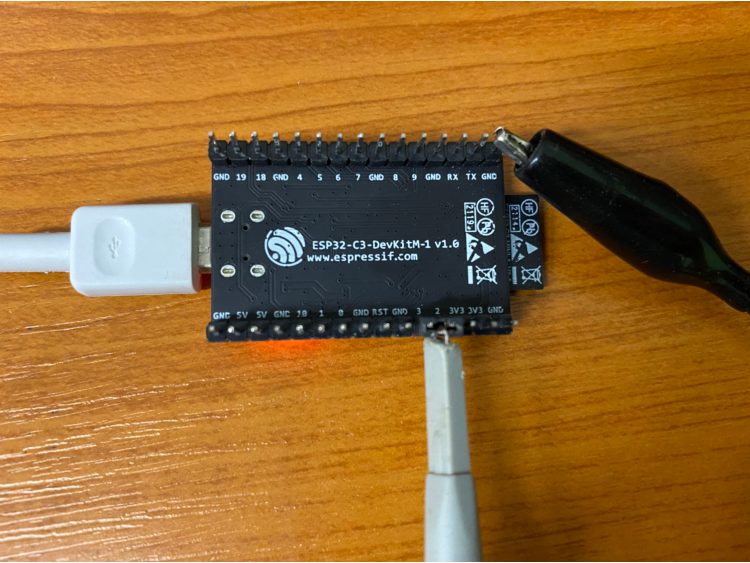
\includegraphics[width=1\textwidth]{images/jumper.pdf}
 \caption{Pin connection via jumper and connection to oscilloscope}
 \end{figure}

 
 After confirmed communication on the pins, the next step was to check the correct bus timing. Without accurate timing on the bus would not be possible to communicate with other stations.
 \clearpage
 
\begin{table}[]
\centering
\begin{tabular}{|c|c|c|c|c|}
\hline
freq     & bit {[}us{]} & Tseg1 {[}-{]} & Tseg2 {[}-{]} & BRP {[}-{]} \\ \hline
125 Kbps & 8            & 15            & 4             & 32          \\ \hline
250 Kbps & 4            & 15            & 4             & 16          \\ \hline
400 Kbps & 2.5          & 16            & 8             & 8           \\ \hline
1 Mbps   & 2            & 15            & 4             & 4           \\ \hline
\end{tabular}
\caption{Bittiming parameters based on frequency}
\label{tab:my-table}
\end{table}

 The measured values were checked for compliance with the signals on the wires.

 \begin{figure}[htb]
 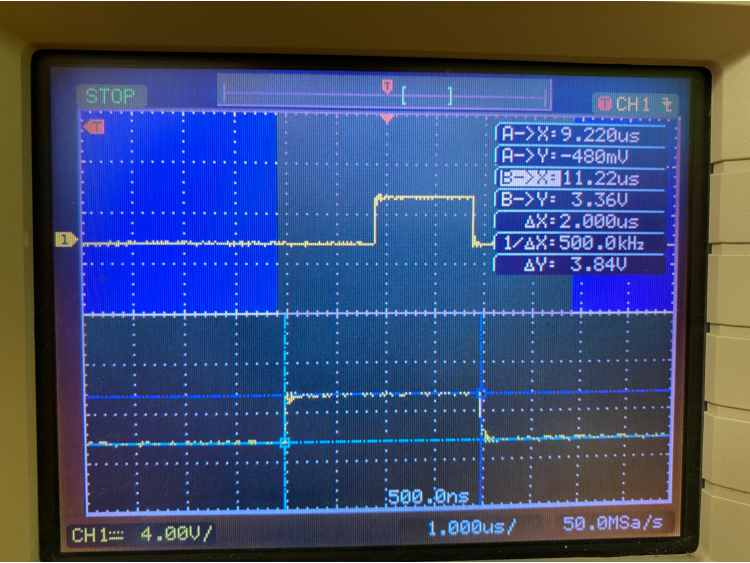
\includegraphics[width=1\textwidth]{images/500Kbps.pdf}
 \caption{Oscilloscope confirmation of correct timing parameters for bitrate 500 Kbps}
 \end{figure}

 Linux provides robust CAN utilities for CAN communication. These Can utilities were used for testing of TWAI driver in standard Operation Mode. For this measurement, the MZ APO board was used. More details about this board are in Section \ref{Sub:connection}.
 
 \clearpage
 \begin{figure}[htb]
 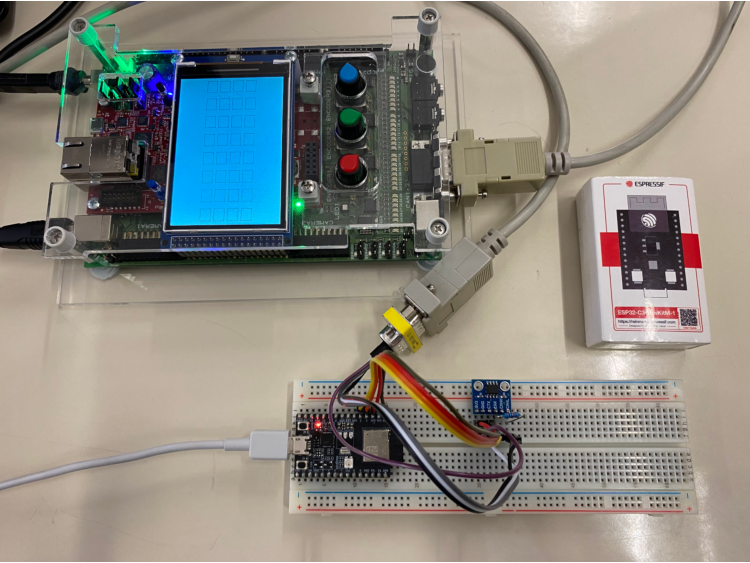
\includegraphics[width=1\textwidth]{images/mz_apo.pdf}
 \caption{Connection with MZ APO board for thorough testing}
 \end{figure}

 \section{Latency tester}
 After simple tests with the newly developed TWAI driver, a possibility for proper automated testing appeared. My colleague Matěj Vaslevski was working on upgrading the Latency tester application for his Master's thesis\cite{thesis-vasilevski}. The Department of Control Engineering CTU FEE has been developing the whole application for several years. The LaTester had to be slightly modified for testing with the "ESP32C3 board". Time accuracy is in microseconds, and the application disposes of several testing modes, all methods of testing are described below, and all resulting graphs are included in the appendix.
The LaTester was initially developed to analyse a Linux-based CAN gateway and its continuous testing. Two independent CAN buses are needed for testing. The principle is as follows: The CAN bus zero generates CAN traffic and records all messages with timestamps. In the optimal case, any board which can run Linux serves as Gateway. This board runs a user-space application, which copies received frames to the CAN bus one. The LaTester records timestamps from frames on CAN bus one and pairs them with previously sent messages. Results are logged to the file with the time differences and statistics.

\clearpage
 \begin{figure}[htb]
 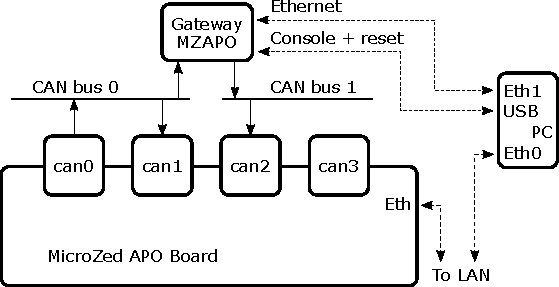
\includegraphics[width=1\textwidth]{images/latester1.pdf}
 \caption{Original connection for LaTester application}
 \end{figure}

 \subsection{Connection}
 \label{Sub:connection}
 The MicroZed APO board served as the PC. At least three CAN IP Cores are required for the proper LaTester functionality. The MZ APO is based on Xilinx Zynq 7000 SoC, and CTU has designed its layout and peripherals of the board. It has two physical CAN IP Cores; therefore, it had to be used CTU CAN FD IP cores designed for FPGA, and four instances were used during testing\cite{ctu-ip-core}. Crossbar connected them on the FPGA. The ESP32-C3 running NuttX RTOS took over the gateway functionality. Unfortunately, only one TWAI (CAN) port is at disposal. Therefore,  the logic of the two buses had to be changed; the newly developed idea worked with one CAN bus and messages distinguished by its ID, not by the CAN bus. The LaTester sent a message with ID $0xA$ and waited for a response with ID one less $0x9$. This rule enforces the priority of transmission from Gateway to get bus access as soon as it processes the received message. The message itself was distinguished the same way as in default mode by increasing the number in the data part. The MZ APO clock settings enable measuring timestamps in CAN IP cores in nanoseconds to an accuracy of ten nanoseconds. It is enough to consider microseconds for the "CAN" communication. \newline
 
 \quad A simple program for NuttX was written, which provides the Gateway functionality. The application was named CAN Ping and firstly opened the CAN interface. Before it started the communication, it changed its priority to a higher level than other programs running in NuttX (from 100 to 110). The rest of the program cycle was to wait for reception of the frame, decrement its ID by one and send it back to the bus. The only exception was ID number zero, which CAN Ping ignored because LaTester used it for its time synchronisation. As for  the LaTester side. it uses standard Linux SocketCAN driver to communicate on the bus.
\clearpage
 \begin{figure}[htb]
 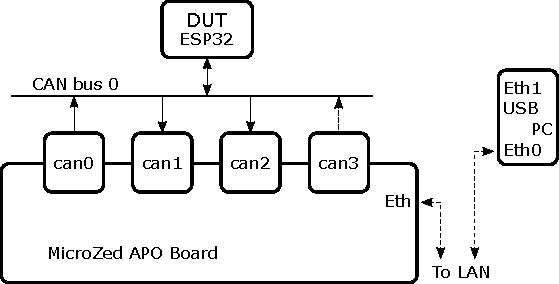
\includegraphics[width=1\textwidth]{images/latester2.pdf}
 \caption{Modified connection for LaTester application with ESP32-C3}
 \end{figure}
 
 Each test has thousands of exchanged messages (3200) and can be divided into several groups. The results are visible in the two tables below. The first table shows measured data for a single transmission per time unit, which means that the following message is not sent earlier than the expected response arrives. The combination for measurement was combined from three bitrate speeds, where 125 Kbps is widely used in automotive or 1 Mbps, the fastest sup-ported speed by ESP32-C3. Messages with different data lengths (2, 4, 8) have been added as an additional dimension.
 
\begin{table}[htb]
    \centering
    \resizebox{\textwidth}{!}{%
    \begin{tabular}{|c|ccl|ccl|ccl|}
    \hline
    \multicolumn{1}{|l|}{} & \multicolumn{2}{c|}{2 data bytes}                                                      & \multicolumn{2}{c|}{4 data bytes}                                                      & \multicolumn{2}{c|}{8 data bytes}                                                      \\ \hline
    bitrate                   & \multicolumn{1}{c|}{avg {[}us{]}} & \multicolumn{1}{c|}{worst {[}us{]}}  & \multicolumn{1}{c|}{avg {[}us{]}} & \multicolumn{1}{c|}{worst {[}us{]}}  & \multicolumn{1}{c|}{avg {[}us{]}} & \multicolumn{1}{c|}{worst {[}us{]}}     \\ \hline
    125 Kbps               & \multicolumn{1}{c|}{0}            & \multicolumn{1}{c|}{0}                  & \multicolumn{1}{c|}{0}            & \multicolumn{1}{c|}{0}               & \multicolumn{1}{c|}{0}            & \multicolumn{1}{c|}{0}                  \\ \hline
    500 Kbps               & \multicolumn{1}{c|}{8}            & \multicolumn{1}{c|}{10}                 & \multicolumn{1}{c|}{8}            & \multicolumn{1}{c|}{10}              & \multicolumn{1}{c|}{10}           & \multicolumn{1}{c|}{12}                 \\ \hline
    1 Mbps                 & \multicolumn{1}{c|}{10}           & \multicolumn{1}{c|}{12}                 & \multicolumn{1}{c|}{10.25}        & \multicolumn{1}{c|}{12}              & \multicolumn{1}{c|}{12}           & \multicolumn{1}{c|}{14}                 \\ \hline
    \end{tabular}%
    }
    \caption{Measured NuttX latencies, messages sent one at a time. 3200 messages were sent.}
    \label{tabulka:nuttx-oneattime}
\end{table}

 The second table shows measurements for a flood of messages. The flood means that the LaTester tries to send each message as fast as possible. However, it must wait before sending the next frame when a message with a lower ID is transmitted from the NuttX. The combinations are similar to the previous case.
 
\begin{table}[htb]
    \centering
    \resizebox{\textwidth}{!}{%
    \begin{tabular}{|c|cc|cc|cc|}
    \hline
             & \multicolumn{2}{c|}{2 data bytes}                                                      & \multicolumn{2}{c|}{4 data bytes}                                                      & \multicolumn{2}{c|}{8 data bytes}                                                      \\ \hline
    freq     & \multicolumn{1}{c|}{avg {[}us{]}} & \multicolumn{1}{c|}{worst {[}us{]}} & \multicolumn{1}{c|}{avg {[}us{]}} & \multicolumn{1}{c|}{worst {[}us{]}}  & \multicolumn{1}{c|}{avg {[}us{]}} & \multicolumn{1}{c|}{worst {[}us{]}}  \\ \hline
    125 Kbps & \multicolumn{1}{c|}{0}            & \multicolumn{1}{c|}{0}              & \multicolumn{1}{c|}{0}            & \multicolumn{1}{c|}{0}               & \multicolumn{1}{c|}{0}            & \multicolumn{1}{c|}{0}               \\ \hline
    500 Kbps & \multicolumn{1}{c|}{132.5}        & \multicolumn{1}{c|}{286}            & \multicolumn{1}{c|}{170.3}        & \multicolumn{1}{c|}{178}             & \multicolumn{1}{c|}{246.2}        & \multicolumn{1}{c|}{250}             \\ \hline
    1 Mbps   & \multicolumn{1}{c|}{66}           & \multicolumn{1}{c|}{141}            & \multicolumn{1}{c|}{85.2}         & \multicolumn{1}{c|}{89}              & \multicolumn{1}{c|}{123.2}        & \multicolumn{1}{c|}{127}             \\ \hline
    \end{tabular}%
    }
    \caption{Measured NuttX latencies, messages sent a flood mode. 3200 messages were sent.}
    \label{tabulka:nuttx-flood}
\end{table}

 The last test was made to check the correct behaviour of threads priorities on ESP32-C3. The wrong setting was simulated by decreasing priority to the CAN Ping application, and the expected values should be worse than in the correct setting. The difference was measured, and it is visible in the graph below that latencies increased.
 
 \begin{figure}[htb]
 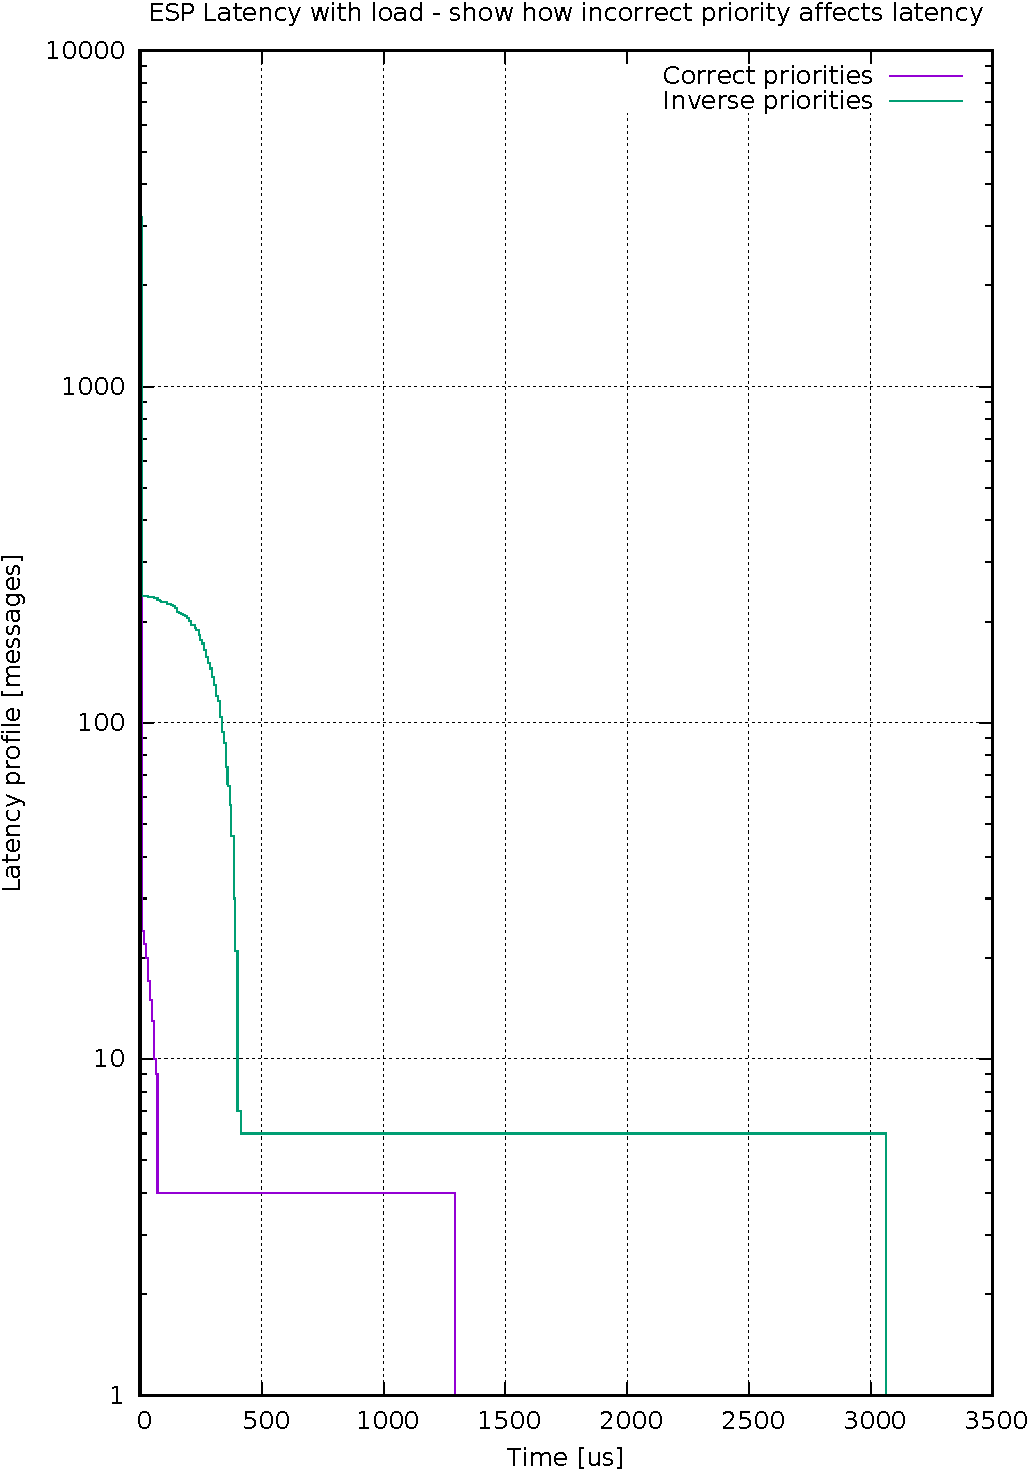
\includegraphics[width=0.7\textwidth]{images/compare_priorities.pdf}
 \caption{Comparison of latencies in correct and inverse priority settings}
 \end{figure}
 
 \section{Motor control}
 One of the suggested testing methods was to use the TWAI driver for PysimCoder based control application. My colleague Dion Beqiri worked on extending Pysimcoder for vector blocks, as well as testing RISC-V board with NuttX and pysimCoder as a Bachelor Thesis\cite{thesis-beqiri}. Mr Beqiri used the ESP32-C3 with pysimCoder and NuttX to control the peripheral to demonstrate his work. There was already an existing project for controlling a 3-phase Permanent Magnet Synchronous Motor with RaspberryPi, which was used as a template for a new NuttX block in pysimCoder. Then hardware was set up by connecting individual pins of the FPGA expansion unit to the ESP32-C3 using jumper cables.
  
 \begin{figure}[htb]
 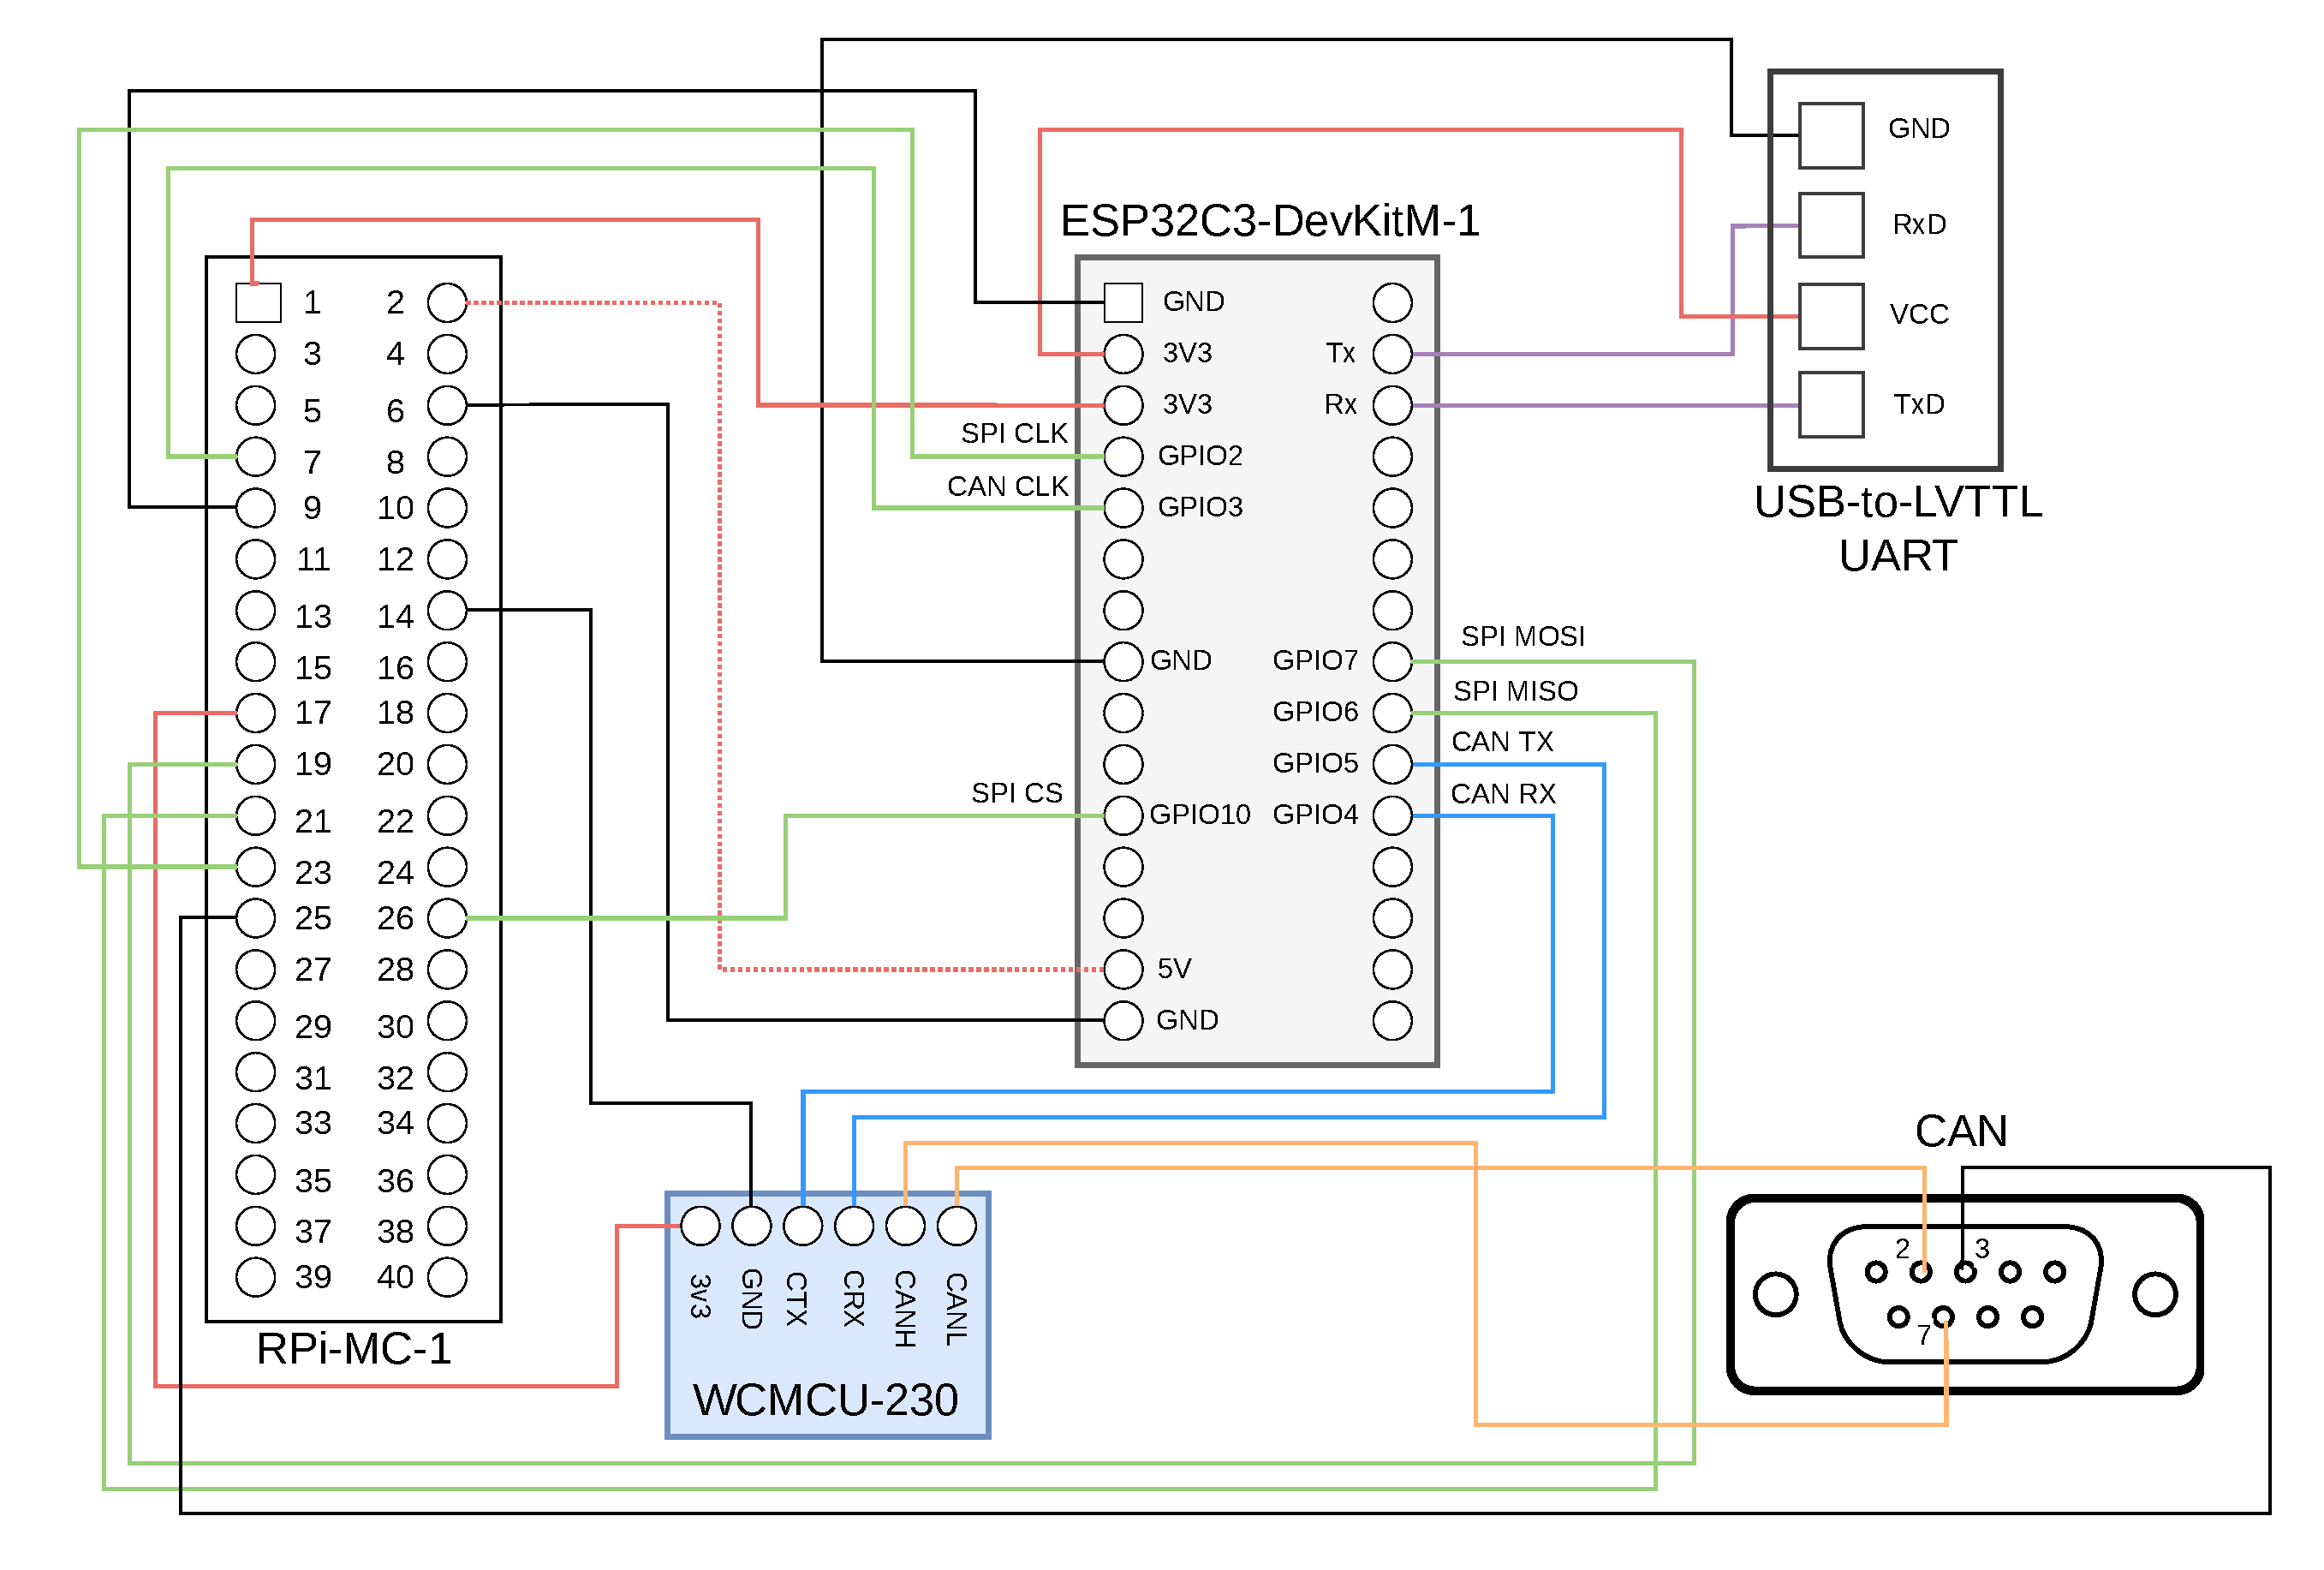
\includegraphics[width=1\textwidth]{images/fpga.pdf}
 \caption{Connection of whole motor control application including TWAI peripheral for CAN communication \cite{thesis-beqiri}}
 \end{figure}
 
Furthermore, connections were made for the CAN signals to send data to a computer. The new NuttX block created for pysimCoder then is tested using this hardware. The block seems to work. However, there is a limitation of the ESP32-C3: it cannot reach a high enough sampling frequency to do PID control. Therefore feedforward simple control diagram has been constructed for it.

 \clearpage
 \begin{figure}[htb]
 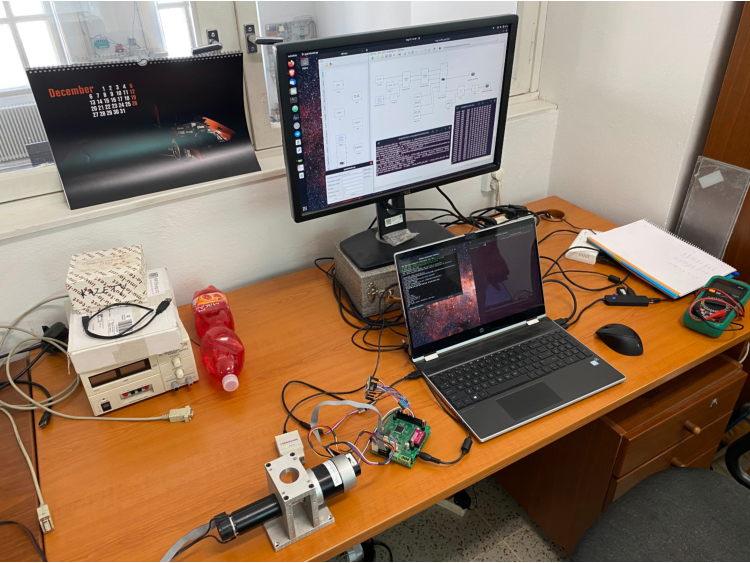
\includegraphics[width=1\textwidth]{images/motor_control.pdf}
 \caption{The physical connection of whole motor control application, including TWAI peripheral on ESP32-C3 for CAN communication in laboratory}
 \end{figure}

 \section{Results}
 All tests passed successfully from the side of the TWAI driver. The TWAI controller communicated with several independent targets, and no problem occurred. It means that no lost messages or incorrect data were observed. Tests focused on proper timing and flooding with messages.
 
 \subsection{LaTester}
 We encountered performance issues on the MZ APO board during a flood of messages on higher bitrates during testing (lost thousands of messages per test) with LaTester. Several CAN IP cores were connected to the bus, and the number of received messages was around ten thousand per second. CAN IP cores raised RX FIFO overflow interrupt, indicating lost messages required for testing. The required results were achieved with several modifications, and the final testing was not affected by the error. What improved the performance was, primarily, the setting of the acceptance filter only for wanted ID (0x9) from NuttX. This lower the rate of RX interrupts and filling of the RX FIFO. The most significant improvement was made when the real-time Linux patch was applied. It helped because it allowed increasing priority for the interrupt handler.

 \subsection{Demonstration of the TWAI driver function with PysimCoder}
 The whole control application worked successfully. The TWAI driver printed the state of the motor to the serial console and data corresponding to the movement.
  \begin{figure}[htb]
 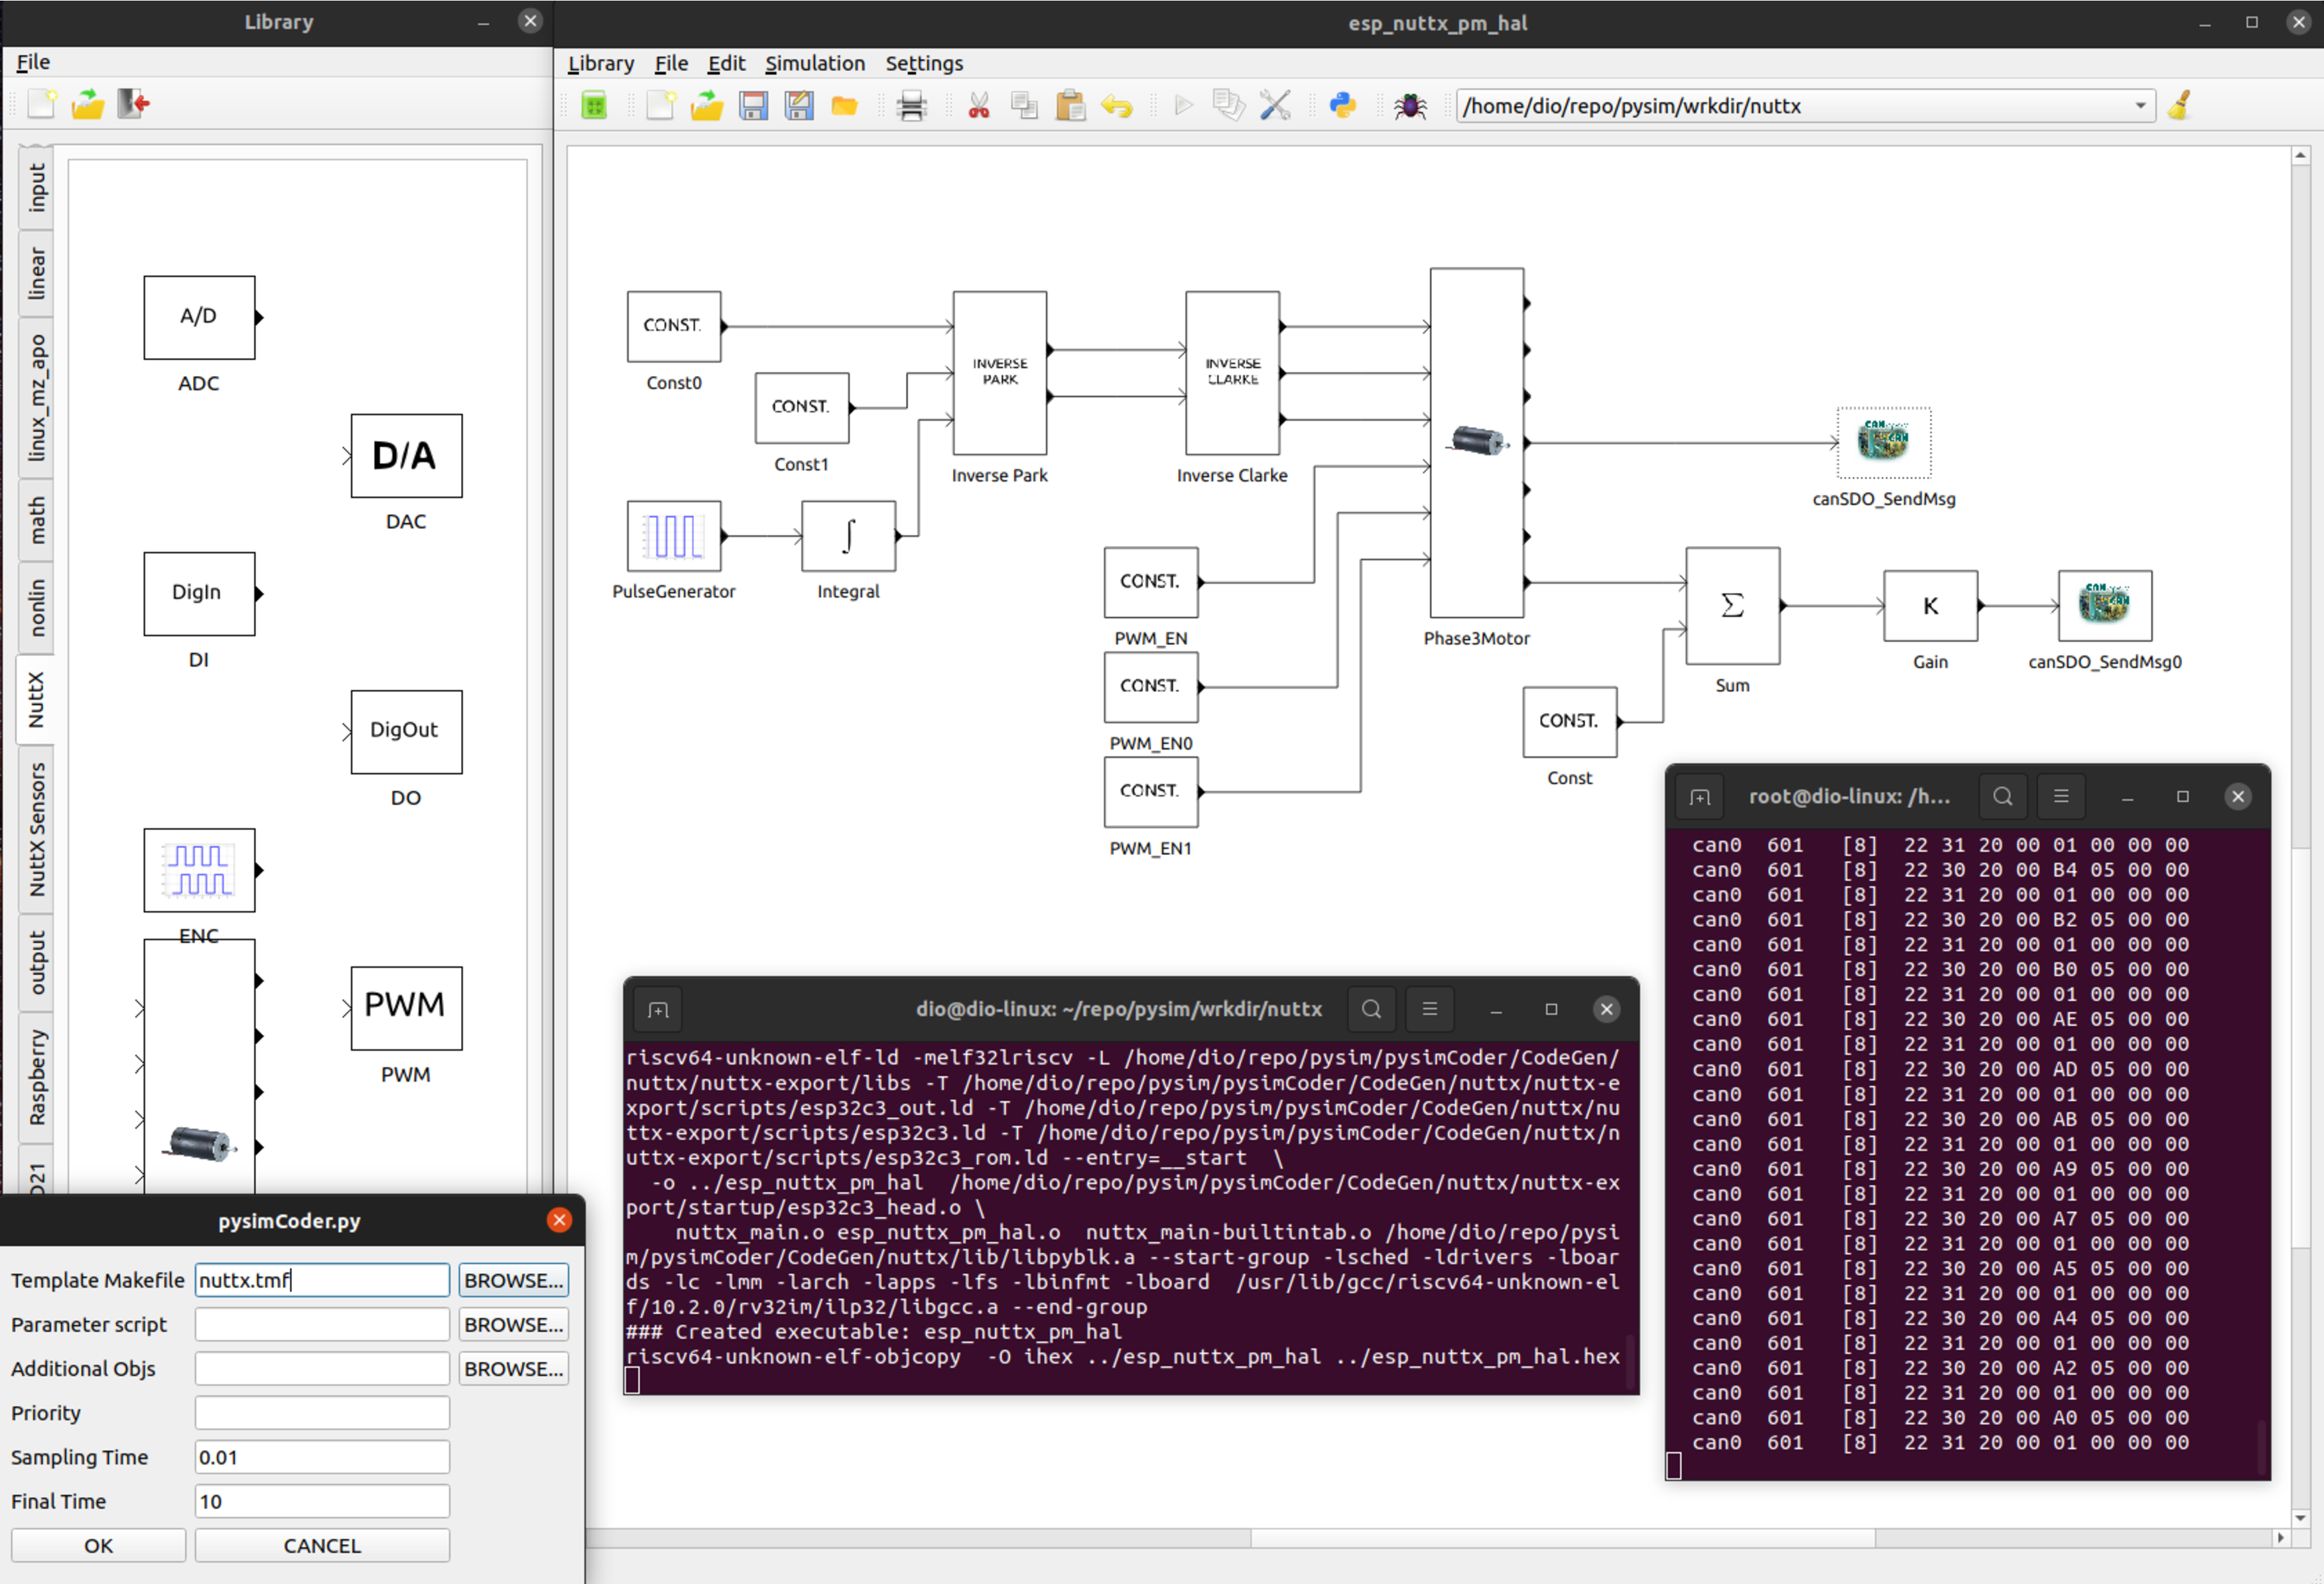
\includegraphics[width=1\textwidth]{images/pysim_nuttx_3pmot_spi_can.pdf}
 \caption{The final layout of the control application in PysimCoder and visible output from the CAN bus \cite{thesis-beqiri}}
 \end{figure}
 

%%%%%%%%%%%%%%%%%%%%%%%%%%%%%%%%%%%%%%
%%%                                %%%
%%%           CHAPTER 8            %%%
%%%                                %%%
%%%%%%%%%%%%%%%%%%%%%%%%%%%%%%%%%%%%%%
 \chapter{Conclusion}
 \label{ch:conclusion}
 The thesis goal was to analyse the driver development process and to contribute with TWAI driver to NuttX RTOS. The TWAI driver for ESP32-C3 was accepted to the mainline, and the result of this work is available in NuttX RTOS\cite{merge}. The created sample configuration demonstrates how to quickly integrate CAN into any application running in NuttX on ESP32-C3. Part of the sample configuration is a NuttX CAN utility application prepared for easy functionality testing.\newline

 \quad The first part of the analysis described CAN technology, including its communication principles. The thesis introduced Espressif's ESP32-C3 hardware description and its official IoT Development Framework ESP-IDF. Principles of Character Device Drivers in NuttX were explained in detail. For the implementation of transmission, it was necessary to know the propagation of user-space application call through the general CAN driver to the architecture-specific TWAI driver and vice versa. A Part of the work was an installation and maintenance guide on working with Espressif's SDK, moreover downloading and working with NuttX. \newline

 \quad All points from the Master's Thesis Assignment were achieved. The TWAI driver was successfully integrated into the NuttX. This required to integrate the TWAI driver in the build and to extend the Kconfig configuration system. The transmission and reception abilities were implemented and tested. The TWAI driver followed requirements for inclusion in the NuttX RTOS and passed all comments during its pull request.\newline

 \quad The driver and its stability and throughput have been successfully tested by a CAN latency tester based on GNU/Linux based system. Usability in PysimCoder generated control system has been verified as well.

 
 \section{Future implementation goals}
  The general CAN driver provides IOCTL calls support in the NuttX. Implementing IOCTL calls in the architecture-specific drivers is not required, and most of them ignore this potential. In the TWAI driver, a bit-timing IOCTL support is implemented, but it is possible to implement the rest of the officially supported IOCTL calls in the future extension. \newline

 \quad 
 Heavy CAN traffic with artificial delay in the driver "RX interrupt" receive handler may cause RX FIFO overrun. In this situation, the last message does not fit into the RX buffer and becomes invalid. TWAI controller does not have any mechanism for discarding the whole RX FIFO. However, the controller has a flag if the current message mapped on Data registers is valid. This information should be sufficient to discard this invalid message and continue. I attempted to write a recovery mechanism, but communication after enforced RX overflow did not recover.\newline

 \quad CAN bus timing is a complex problem, and it is difficult to calculate all the parameters optimally. The actual implementation in the TWAI driver behaves similarly to the modern Linux solution. There is a potential for improvement because rate error is the only criteria parameter for a final solution. Adding an extension of the optimal parameter set suitable for a particular controller could improve timing parametrisation.
 
 
\renewcommand\bibname{References}
\begin{thebibliography}{1}
\bibitem{risc-v} David A. Patterson and John L. Hennessy. 2017. Computer Organization and Design RISC-V Edition: The Hardware Software Interface (1st. ed.). Morgan Kaufmann Publishers Inc., San Francisco, CA, USA.
\bibitem{history} J. Palomino, E. Cuty and A. Huanachin, "Development of a CAN Bus datalogger for recording sensor data from an internal combustion ECU," 2021 IEEE International Workshop of Electronics, Control, Measurement, Signals and their application to Mechatronics (ECMSM), 2021, pp. 1-4, doi: 10.1109/ECMSM51310.2021.9468837.
\bibitem{can_fd} G. Marcon Zago and E. Pignaton de Freitas, "A Quantitative Performance Study on CAN and CAN FD Vehicular Networks," in IEEE Transactions on Industrial Electronics, vol. 65, no. 5, pp. 4413-4422, May 2018, doi: 10.1109/TIE.2017.2762638.
\bibitem{can_subsystem} Dr. Oliver Hartkopp, The CAN networking subsystem of the Linux kernel, https://www.can-cia.org/fileadmin/resources/documents/proceedings/2012\text{-}hartkopp.pdf, accessed: 2022-05-20.
\bibitem{can_frame} Dr. Oliver Hartkopp, The CAN Subsystem of the Linux Kernel, https://wiki.automotivelinux.org/\text{-}media/agl-distro/agl2017-socketcan-print.pdf by Oliver Hartkopp - page 2, accessed: 2022-05-19.
\bibitem{can_physical} Pavel Pisa, GNU/Linux, CAN and CANopen in Real-time Control Applications by Pavel Pisa - page 10, https://www.linuxdays.cz/2017/video/Pavel\text{-}Pisa-CAN\text{-}canopen.pdf, accessed: 2022-05-19.
\bibitem{can-course} doc. Ing. Jiří Novák, Ph.D., Computer Communication Interfaces course on CTU FEE BE4M38KRP, Controller Area Network - Presentation, accessed: 2022-05-19.
\bibitem{thesis-vasilevski} Matěj Vasilevski - Master's Thesis, CAN Bus Latency Test Automation for Continuous Testing and Evaluation, May 2022
\bibitem{thesis-beqiri} Dion Beqiri -Bachelor Thesis, Open Rapid Control Prototyping, Education and Design Tools, May 2022, https://github.com/beqirdio/pysimCoder-thesis\text{-}DB
\bibitem{bachelor-thesis} Jan Charvát, Model of CAN FD Communication Controller for QEMU Emulator, https://dspace.cvut.cz/bitstream/handle/10467/87714/F3-BP-2020-
Charvat-Jan-
Model\text{-}of\text{-}CAN\text{-}FD\text{-}
Communication\text{-}Controller\text{-}
for\text{-}QEMU\text{-}Emulator.pdf, accessed: 2022-05-19.
\bibitem{qemu} QEMU, CAN Bus Emulation Support, https://www.qemu.org/docs/master/system/devices/can.html, accessed: 2022-05-19.
\bibitem{can_filter} CAN in Automation, CAN protocol implementations, https://www.can-cia.org/can-knowledge/can/can-implementations/, accessed: 2022-05-11.
\bibitem{esp32c3-devkit} Espressif Systems, ESP32-C3-DevKitM-1, https://docs.espressif.com/projects/esp-idf/en/v4.4/esp32c3/hw-reference/esp32c3/user-guide-devkitm-1.html, accessed: 2022-05-20.
\bibitem{otrees} Jan Charvát, esp32c3 m1 nuttx, arcticle written during the writing of the Maste's Thesis, https://gitlab.fel.cvut.cz/otrees/risc-v-esp32/work-and-ideas/-/wikis/esp32c3-m1-nuttx, accessed: 2022-05-20.
\bibitem{esp-idf} Espressif Systems, Official IoT Development Framework, https://www.espressif.com/en/products/sdks/esp-idf, accessed: 2022-05-20.
\bibitem{esp32-c3-mcu} Espressif Systems, ESP32-C3-MINI-1 ESP32-C3-MINI-1U Datasheet, https://www.espressif.com/sites/default/files/documentation/esp32-c3-mini-1\text{-}datasheet\text{-}en.pdf, accessed: 2022-01-20.
\bibitem{esp-idf-guide} Espressif Systems, ESP-IDF Programming Guide, https://docs.espressif.com/projects/esp-idf/en/v4.4/esp32c3/index.html, accessed: 2022-05-20.
\bibitem{esp-idf-git} Espressif Systems, esp-idf, https://github.com/espressif/esp-idf, accessed: 2022-05-20.
\bibitem{esp-idf-intallers} Espressif Systems, ESP-IDF Windows Installer Download, https://dl.espressif.com/dl/esp-idf/?idf=4.4, accessed: 2022-05-20.
\bibitem{esp-idf-bootloader} Espressif Systems, esp-nuttx-bootloader, https://github.com/espressif/esp-nuttx-bootloader/releases, accessed: 2022-05-20.
\bibitem{ecu} CSS Electronics, CAN BUS EXPLAINED - A SIMPLE INTRO (2020), https://www.csselectronics.com/screen/page/simple-intro-to-can-bus/language/en, accessed: 2022-05-20.
\bibitem{nuttx_about} The Apache Software Foundation, About Apache NuttX, https://nuttx.apache.org/docs/latest/introduction/about.html, accessed: 2022-05-11.
\bibitem{nuttx_protected} The Apache Software Foundation, NuttX Protected Build,  https://cwiki.apache.org/confluence/display/NUTTX/NuttX+Protected+Build, accessed: 2022-05-11.
\bibitem{zephyr} Zephyr Project, https://www.zephyrproject.org/, accessed: 2022-05-11.
\bibitem{mbed} Mbed OS, https://os.mbed.com/, accessed: 2022-05-11.
\bibitem{nuttx_start} The Apache Software Foundation, Getting Started, https://nuttx.apache.org/docs/latest/quickstart/index.html, accessed: 2022-05-11.
\bibitem{kconfig} The kernel development community, Kconfig Language, https://www.kernel.org/doc/html/latest/kbuild/kconfig-language.html, accessed: 2022-05-11.
\bibitem{socketcan} Wikimedia Foundation, Inc., SocketCAN, https://en.wikipedia.org/wiki/File:Socketcan.png, accessed: 2022-05-11.
\bibitem{sifive} SiFive, Inc., freedom-tools, https://github.com/sifive/freedom-tools/releases, accessed: 2022-05-11.
\bibitem{license_bsd} White Source, Top 8 BSD License’s Questions Answered, https://www.whitesourcesoftware.com/resources/blog/top-8-bsd-licenses-questions-answered/, accessed: 2022-05-11.
\bibitem{license_apache} The Apache Software Foundation, FREQUENT QUESTIONS ABOUT APACHE LICENSING, https://www.apache.org/foundation/license-faq.html, accessed: 2022-05-11.
\bibitem{esp32c3-trm} Espressif Systems, ESP32-C3 Technical Reference Manual,
https://www.espressif.com/sites/default/files/documentation/esp32-c3\text{-}technical\text{-}reference\text{-}manual\text{-}en.pdf, accessed: 2022-01-20.
\bibitem{lincan} Pavel Pisa, Linux/RT-Linux CAN Driver (LinCAN), https://cmp.felk.cvut.cz/~pisa/can/doc/lincandoc-0.3.pdf, accessed: 2022-05-20.
\bibitem{lincan-code} Pavel Pisa, Linux/RT-Linux CAN Driver (LinCAN), https://sourceforge.net/p/ortcan/lincan/ci/master/tree/lincan/src/c\text{-}can.c, accessed: 2022-05-20.
\bibitem{sja-1000} NXP, SJA1000 Stand-alone CAN controller, https://www.nxp.com/docs/en/application-note/AN97076.pdf, accessed: 2022-05-20.
\bibitem{twai-branch} Jan Charát - charvj10 fork of NuttX, incubator-nuttx, https://github.com/charvj/incubator-nuttx/tree/esp32c3-twai, accessed: 2022-01-20.
\bibitem{ctu-ip-core} CAN with Flexible Data-rate IP Core developed at Department of Measurement of FEE CTU, CTU CAN FD IP Core, https://gitlab.fel.cvut.cz/canbus/ctucanfd\text{-}ip\text{-}core, accessed: 2022-01-20.
\bibitem{nuttx-mainline} The Apache Software Foundation, incubator-nuttx, https://github.com/apache/incubator-nuttx, accessed: 2022-01-20.
\bibitem{merge} The Apache Software Foundation, incubator-nuttx, https://github.com/apache/incubator-nuttx/pull/6005, accessed: 2022-01-20.

\end{thebibliography}

\appendix
\chapter{Detail results from LaTester}
 Here is a set of graphs showing in detail the measurement results with the LaTester. These graphs are shared output from our work with Matěj Vasilevski.
  
  \begin{figure}[htb]
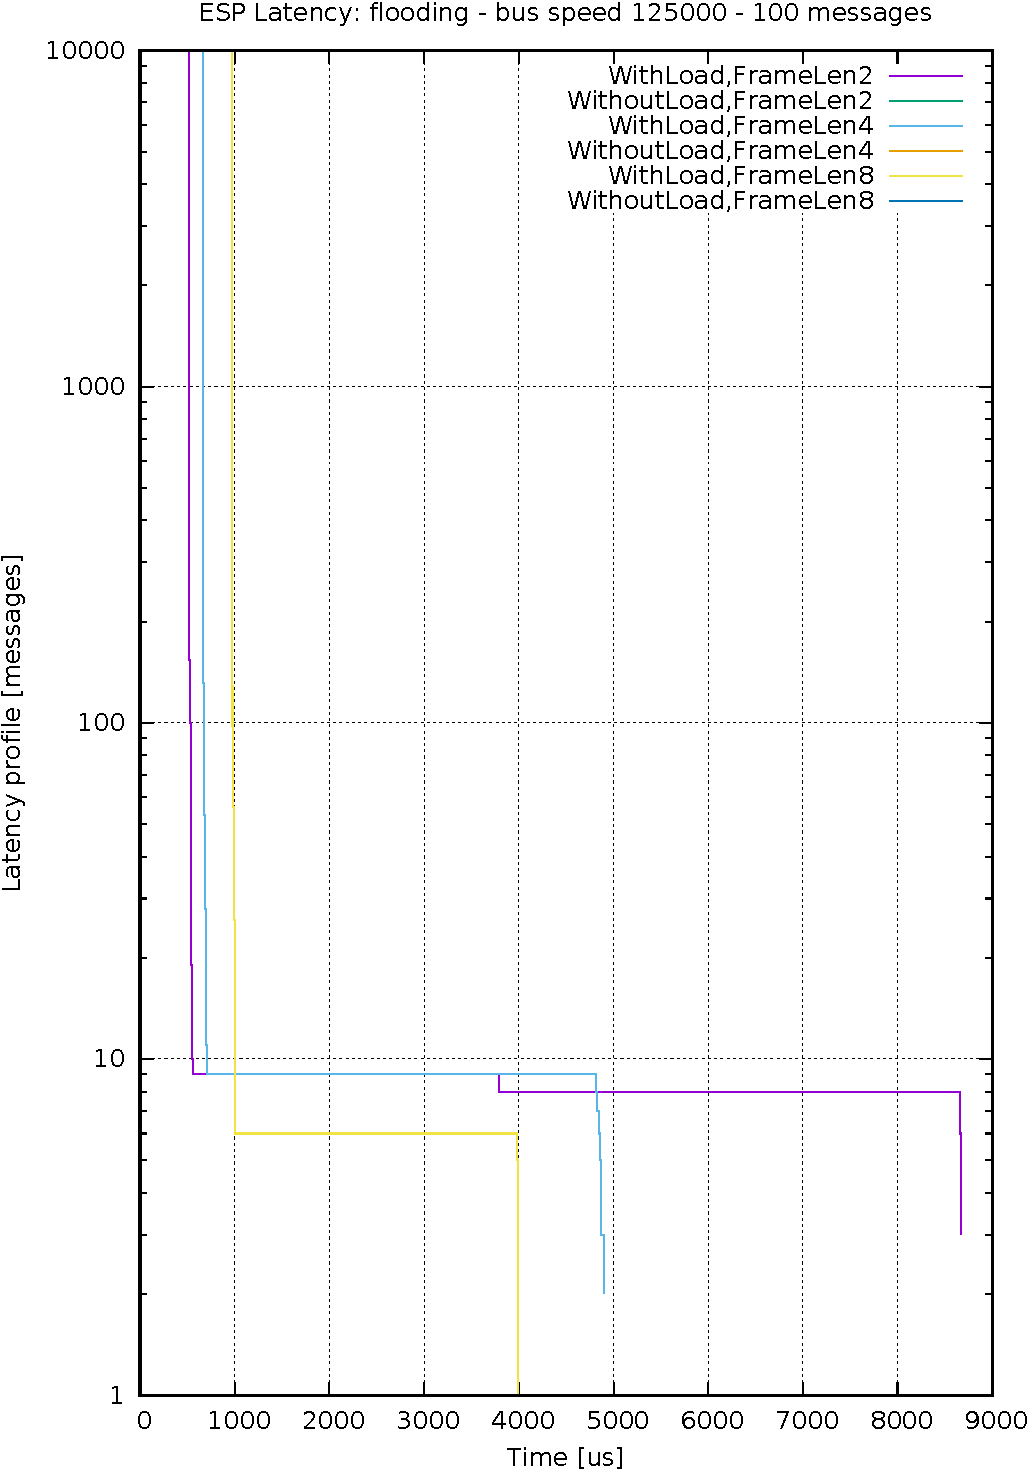
\includegraphics[width=\linewidth]{figures/speed125000_messages100_floodTrue.pdf}
\caption{ESP latency profile: flooding - bus speed 125000 - 100 messages}
\end{figure}

\begin{figure}[htb]
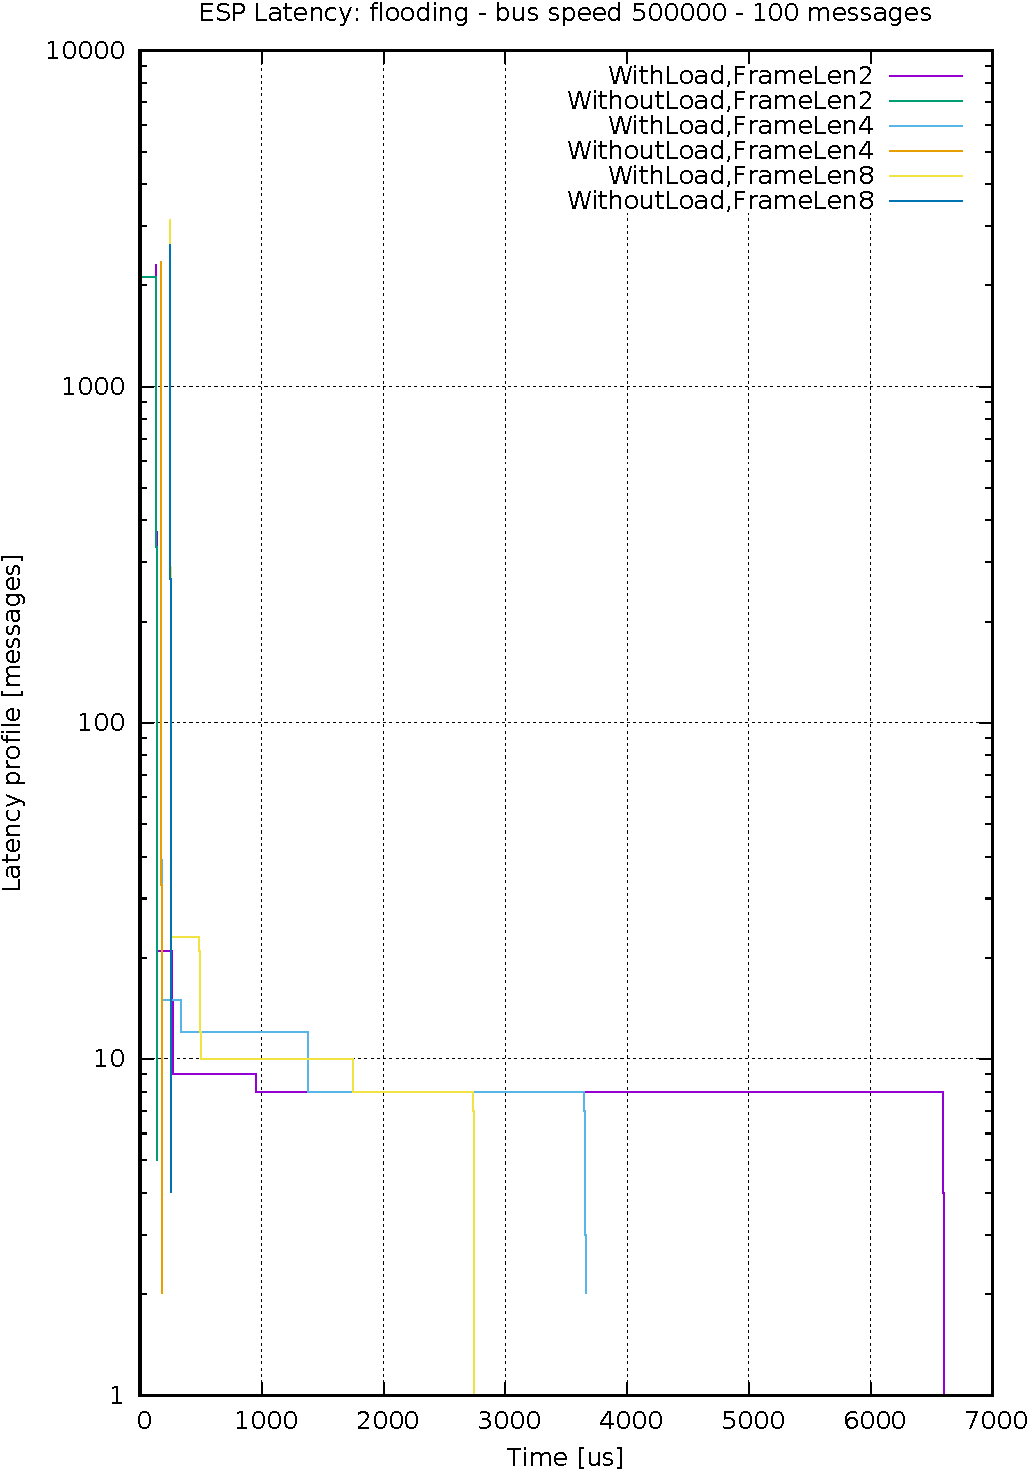
\includegraphics[width=\linewidth]{figures/speed500000_messages100_floodTrue.pdf}
\caption{ESP latency profile: flooding - bus speed 500000 - 100 messages}
\end{figure}

\begin{figure}[htb]
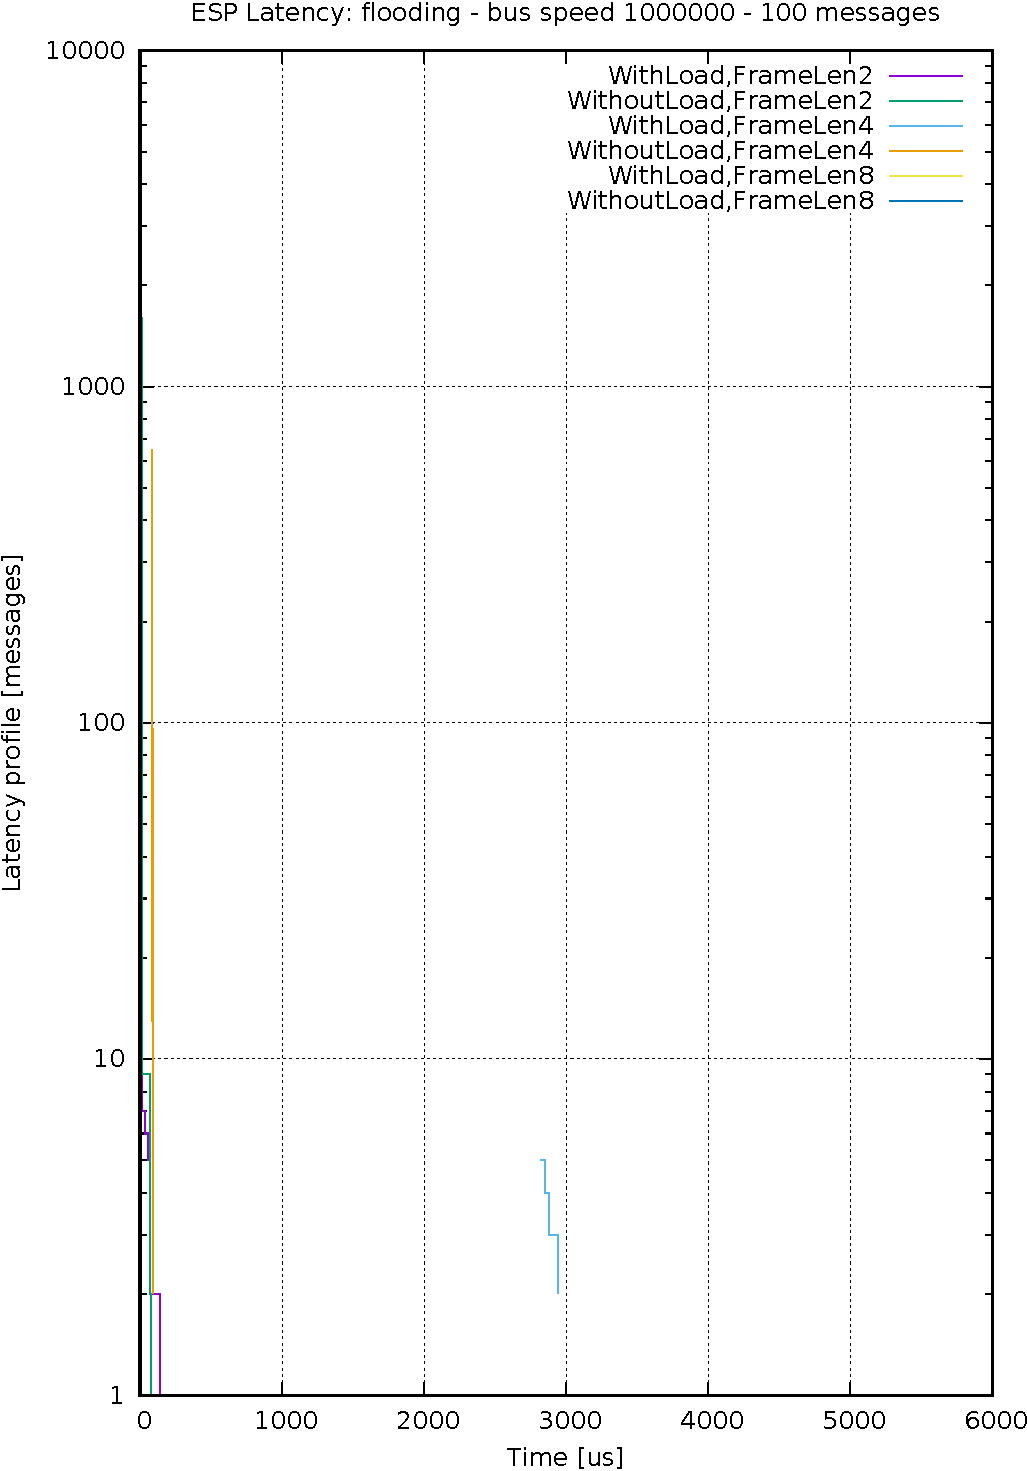
\includegraphics[width=\linewidth]{figures/speed1000000_messages100_floodTrue.pdf}
\caption{ESP latency profile: flooding - bus speed 1000000 - 100 messages}
\end{figure}

\begin{figure}[htb]
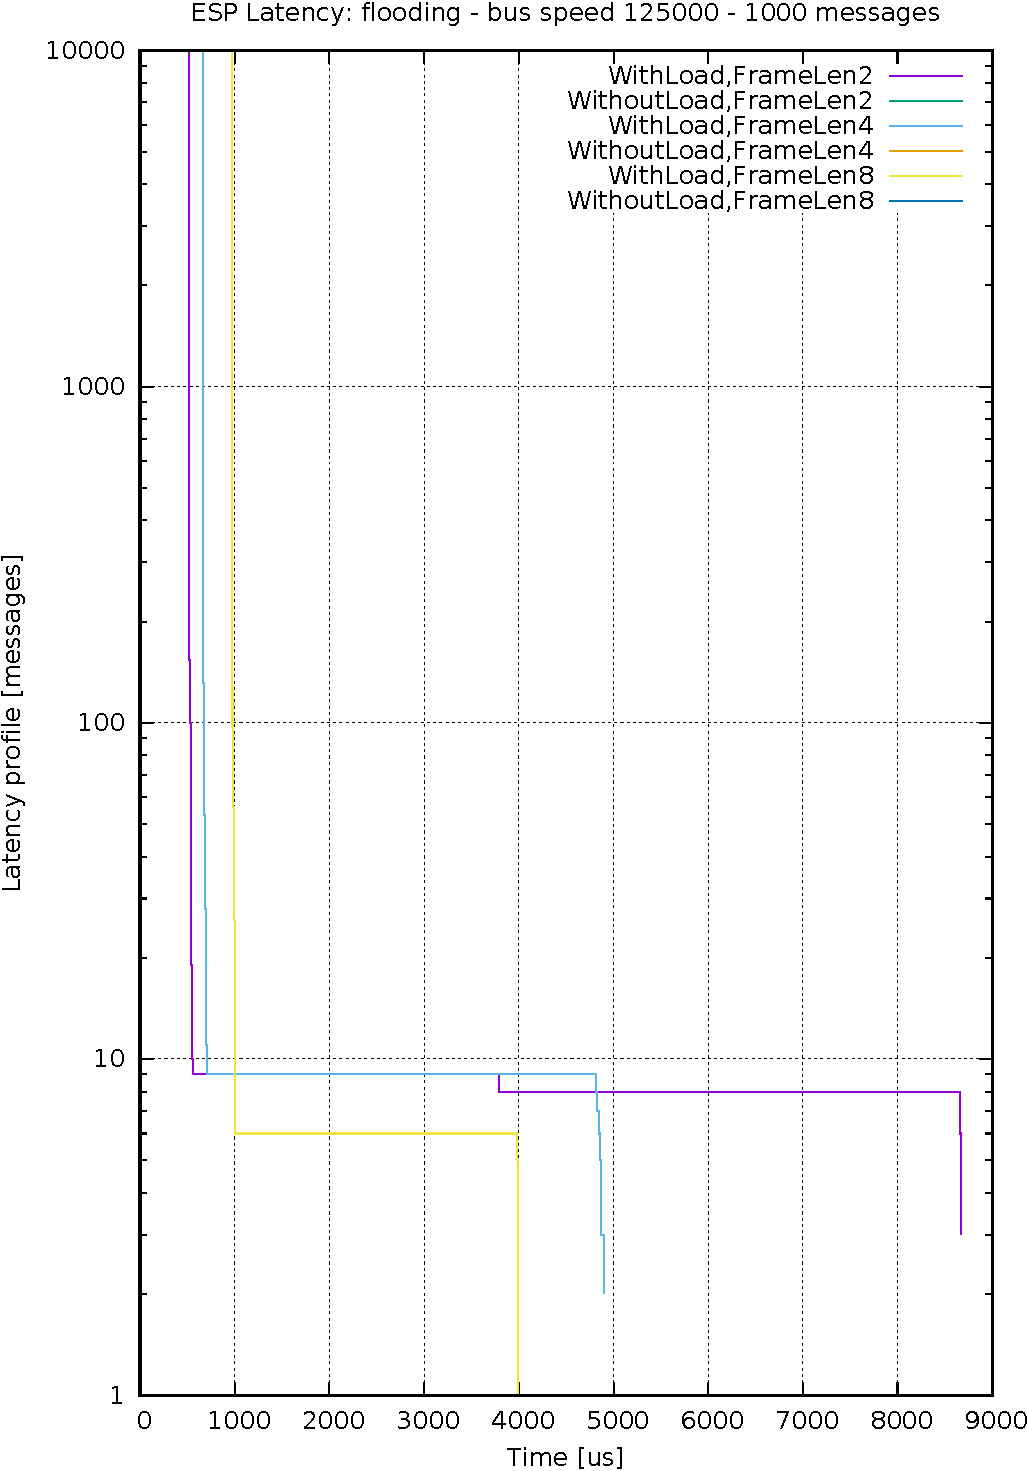
\includegraphics[width=\linewidth]{figures/speed125000_messages1000_floodTrue.pdf}
\caption{ESP latency profile: flooding - bus speed 125000 - 1000 messages}
\end{figure}

\begin{figure}[htb]
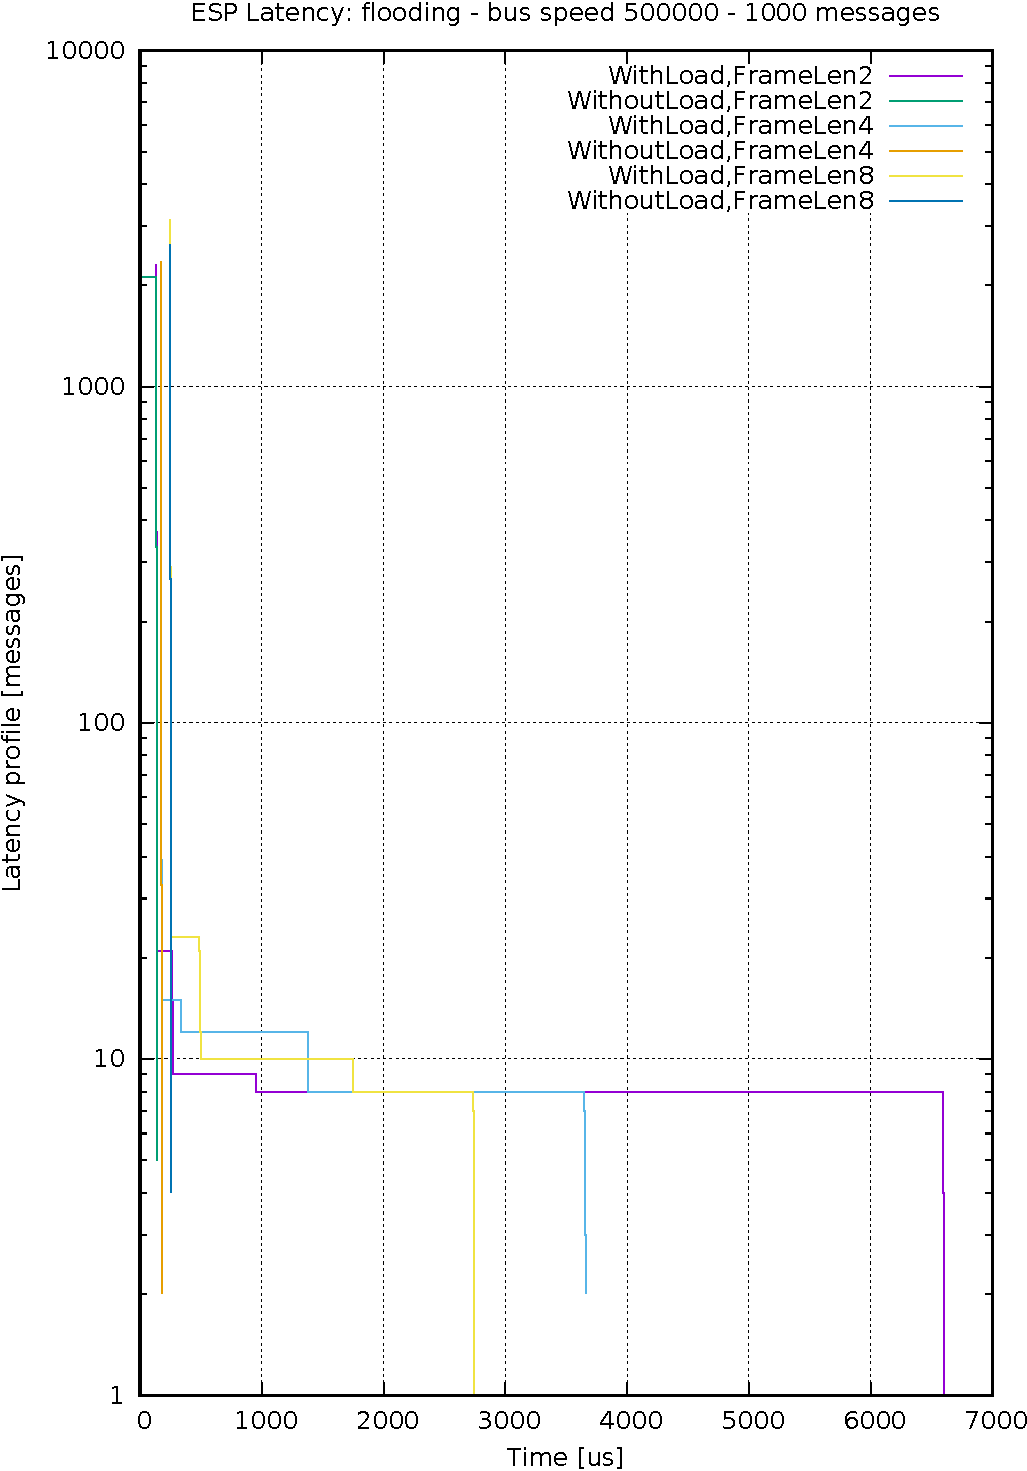
\includegraphics[width=\linewidth]{figures/speed500000_messages1000_floodTrue.pdf}
\caption{ESP latency profile: flooding - bus speed 500000 - 1000 messages}
\end{figure}

\begin{figure}[htb]
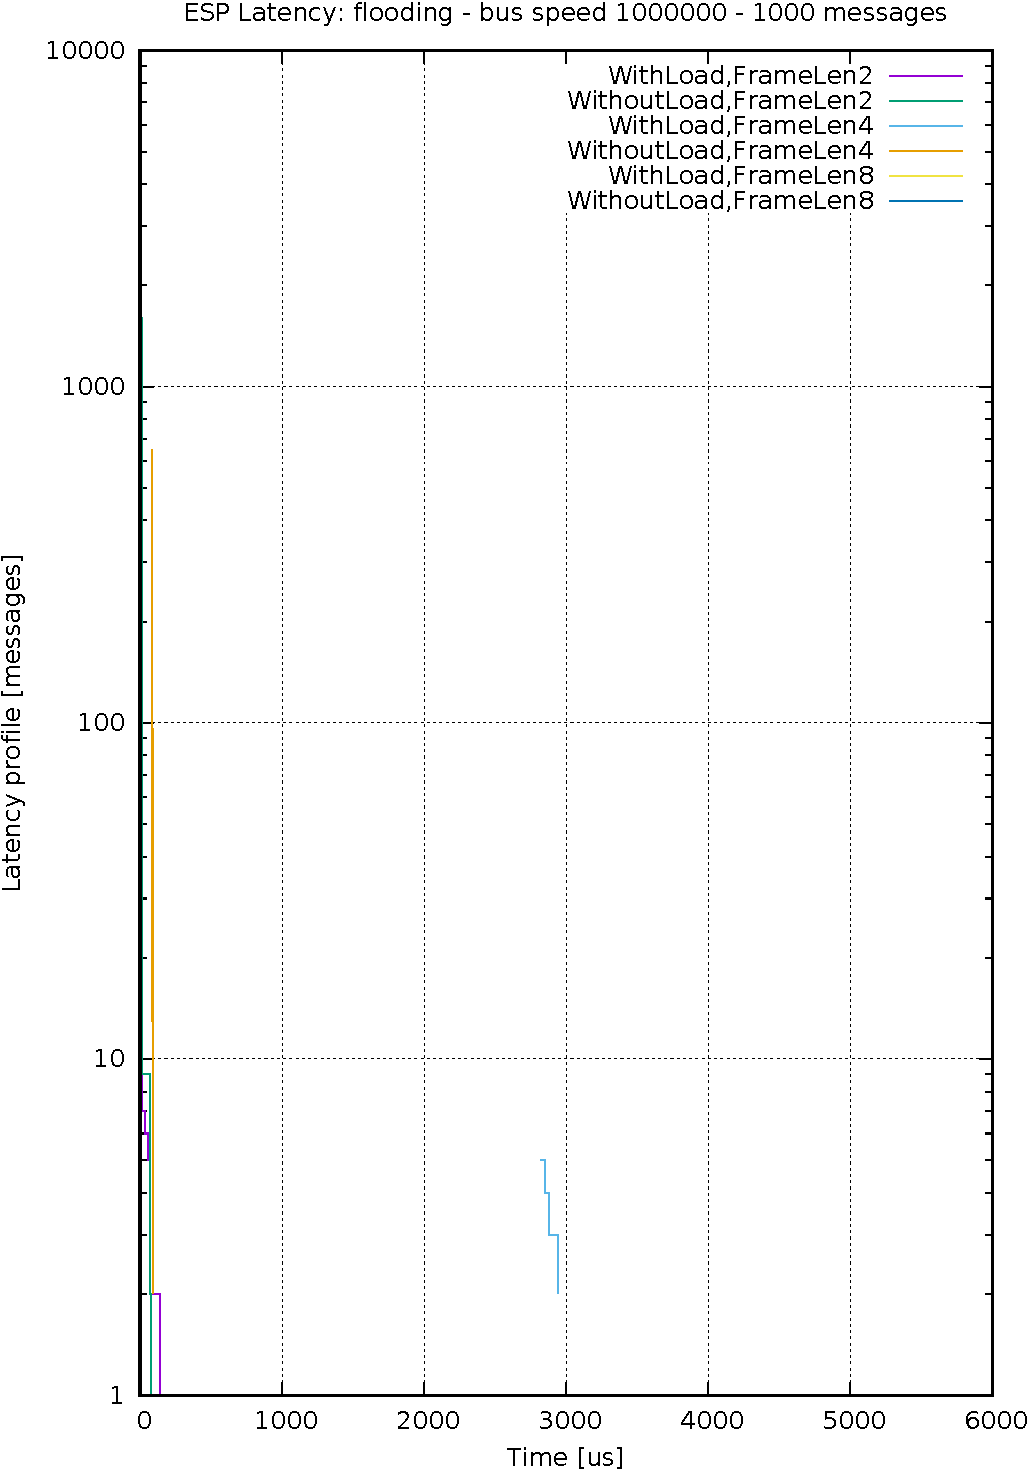
\includegraphics[width=\linewidth]{figures/speed1000000_messages1000_floodTrue.pdf}
\caption{ESP latency profile: flooding - bus speed 1000000 - 1000 messages}
\end{figure}

\begin{figure}[htb]
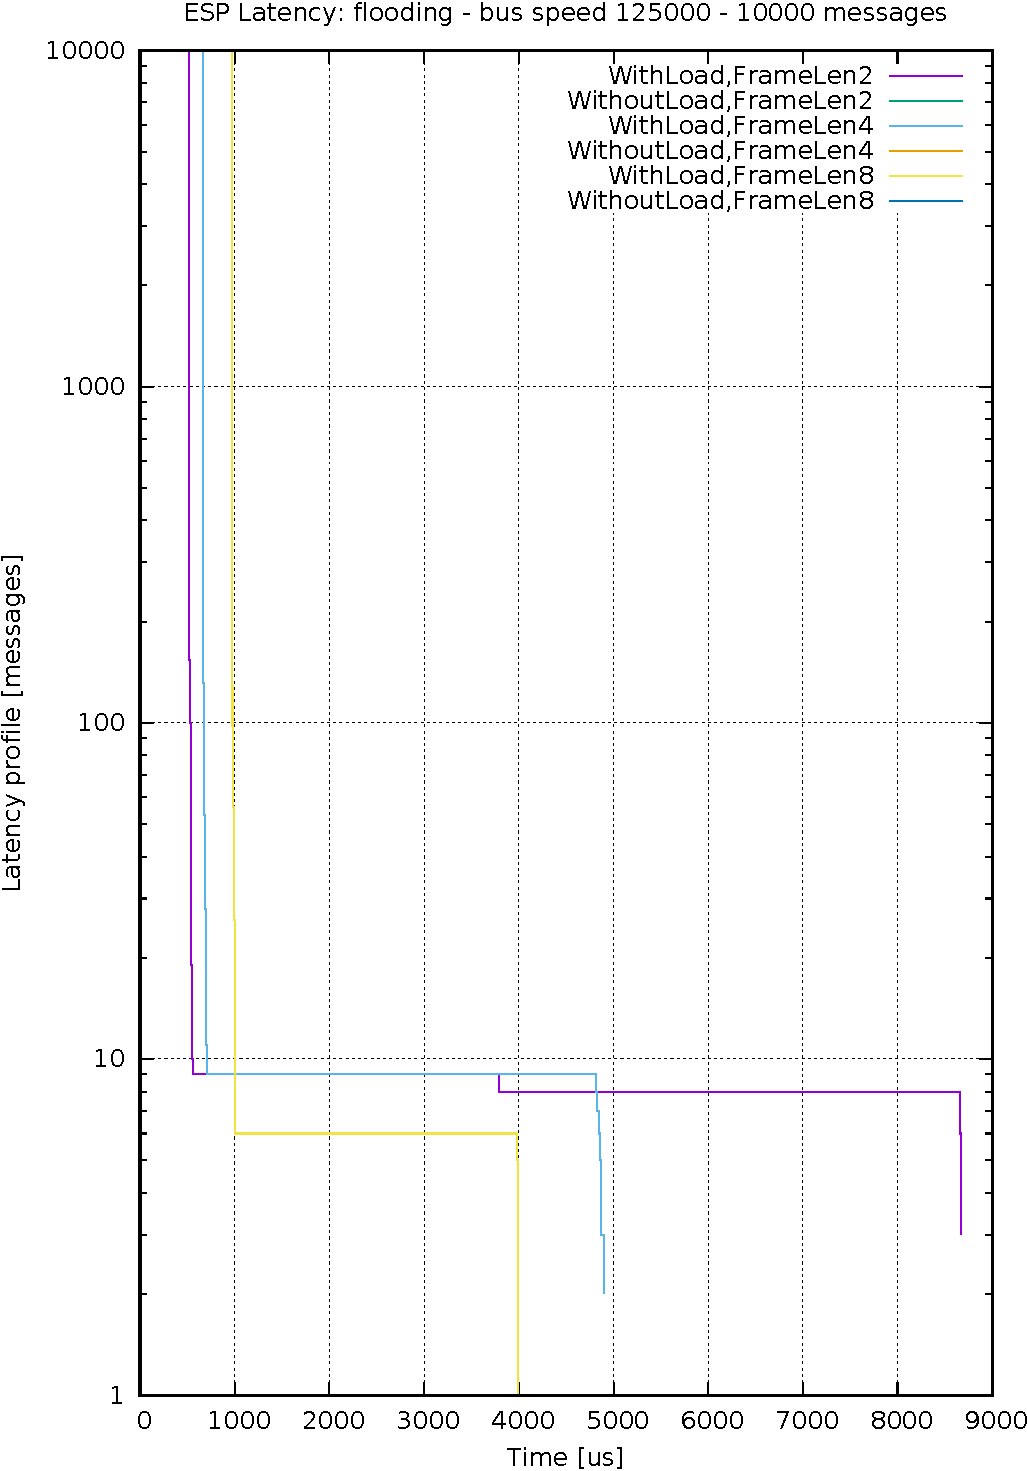
\includegraphics[width=\linewidth]{figures/speed125000_messages10000_floodTrue.pdf}
\caption{ESP latency profile: flooding - bus speed 125000 - 10000 messages}
\end{figure}

\begin{figure}[htb]
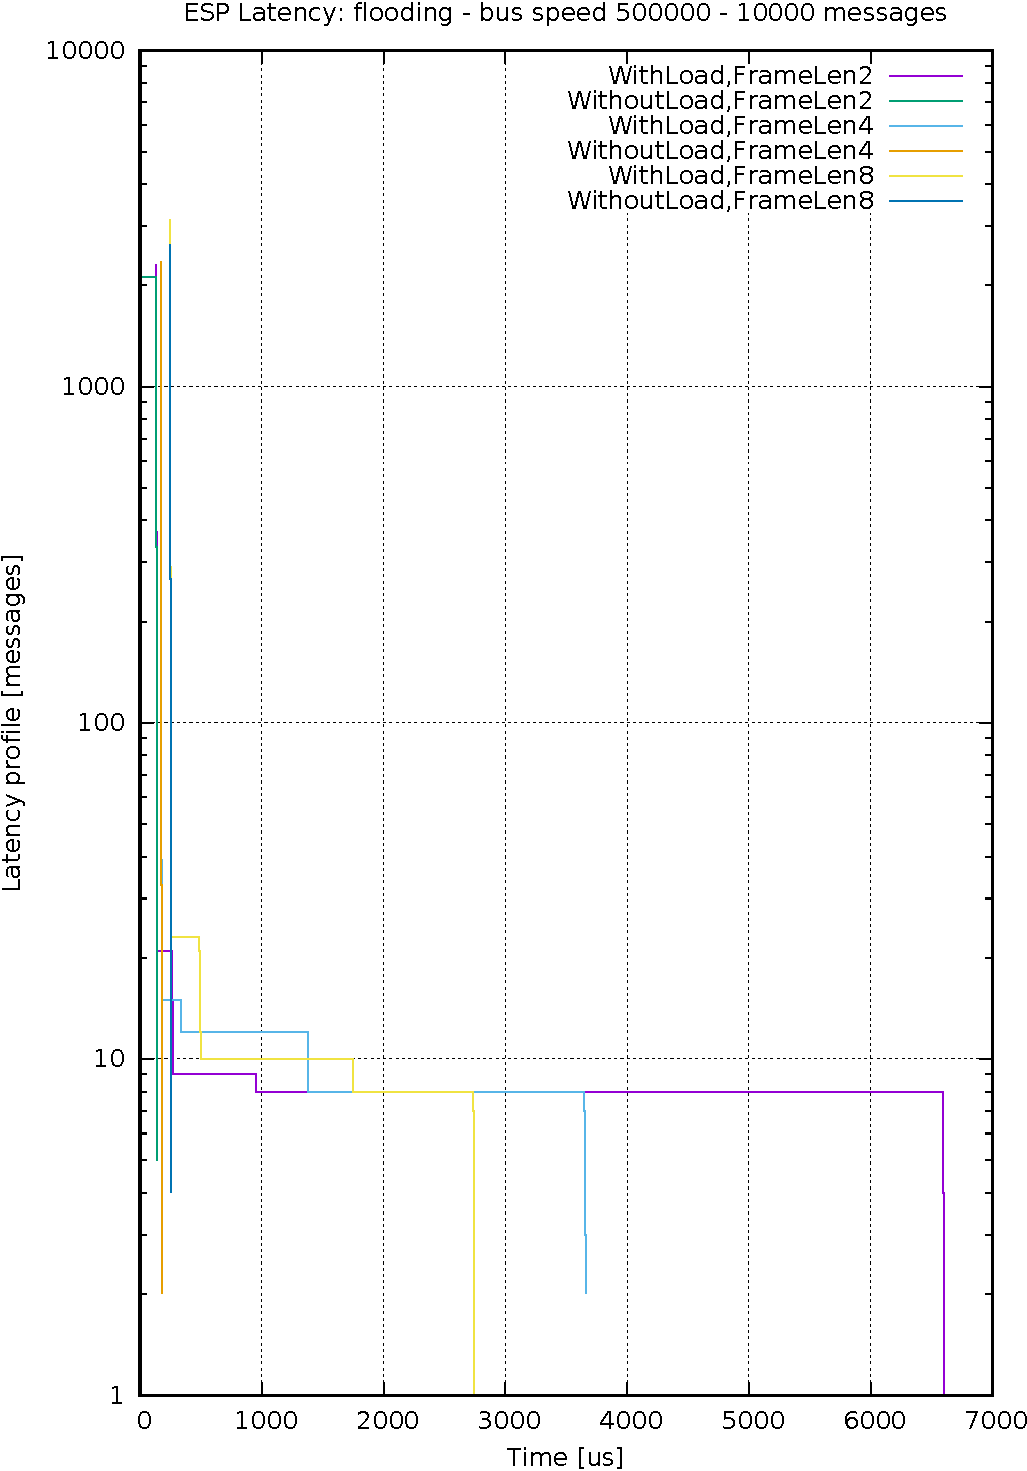
\includegraphics[width=\linewidth]{figures/speed500000_messages10000_floodTrue.pdf}
\caption{ESP latency profile: flooding - bus speed 500000 - 10000 messages}
\end{figure}

\begin{figure}[htb]
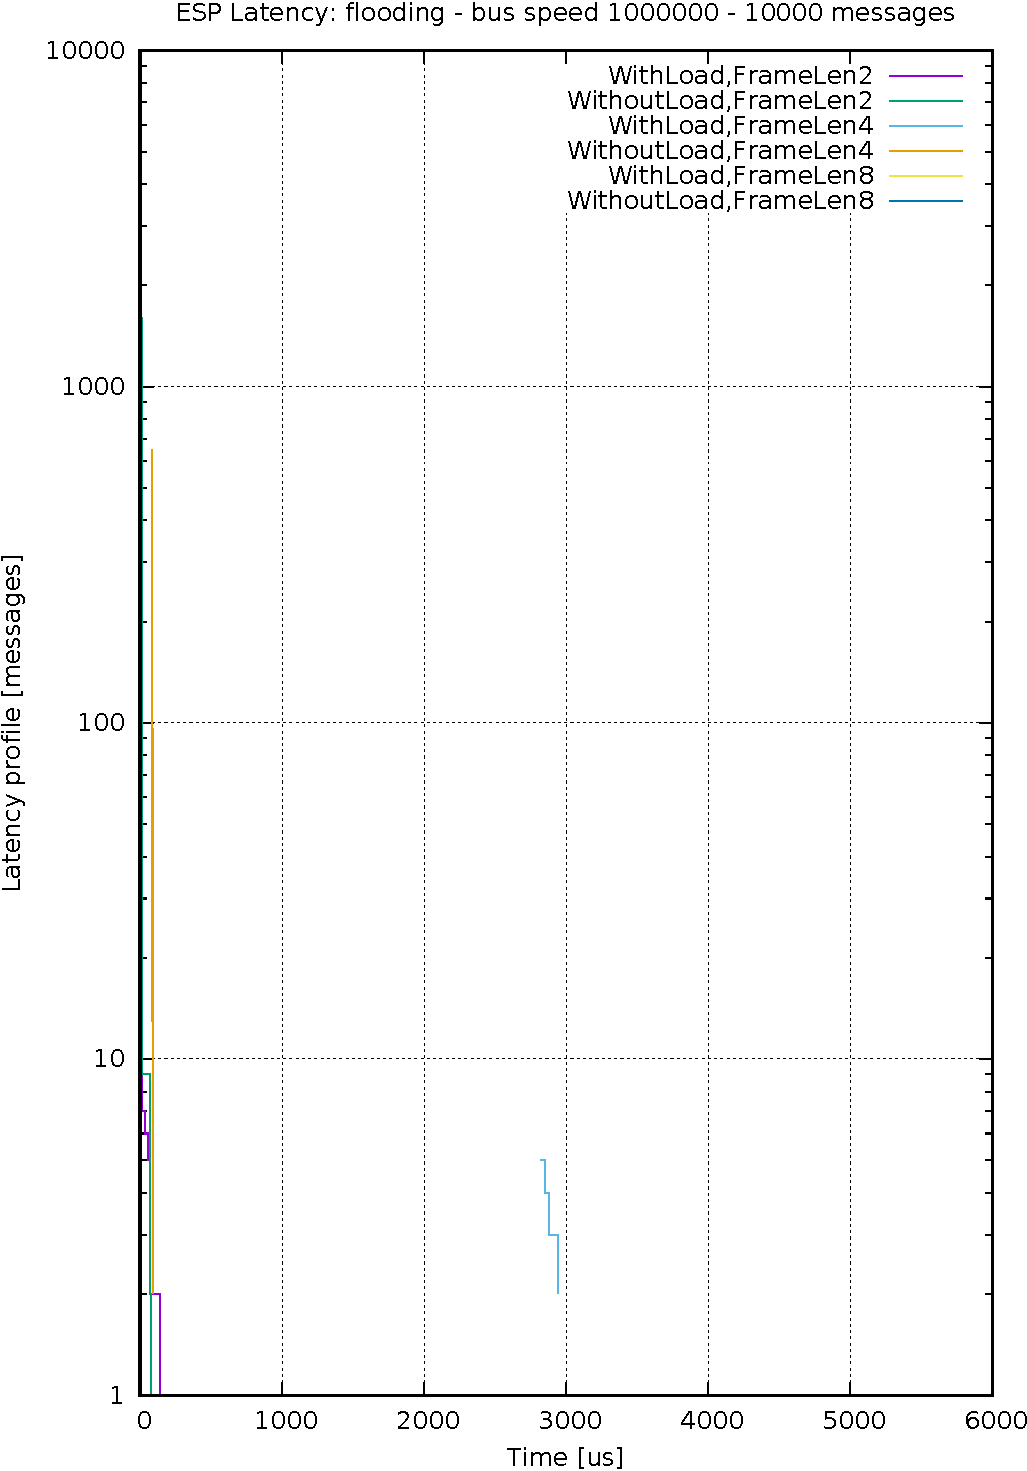
\includegraphics[width=\linewidth]{figures/speed1000000_messages10000_floodTrue.pdf}
\caption{ESP latency profile: flooding - bus speed 1000000 - 10000 messages}
\end{figure}

\begin{figure}[htb]
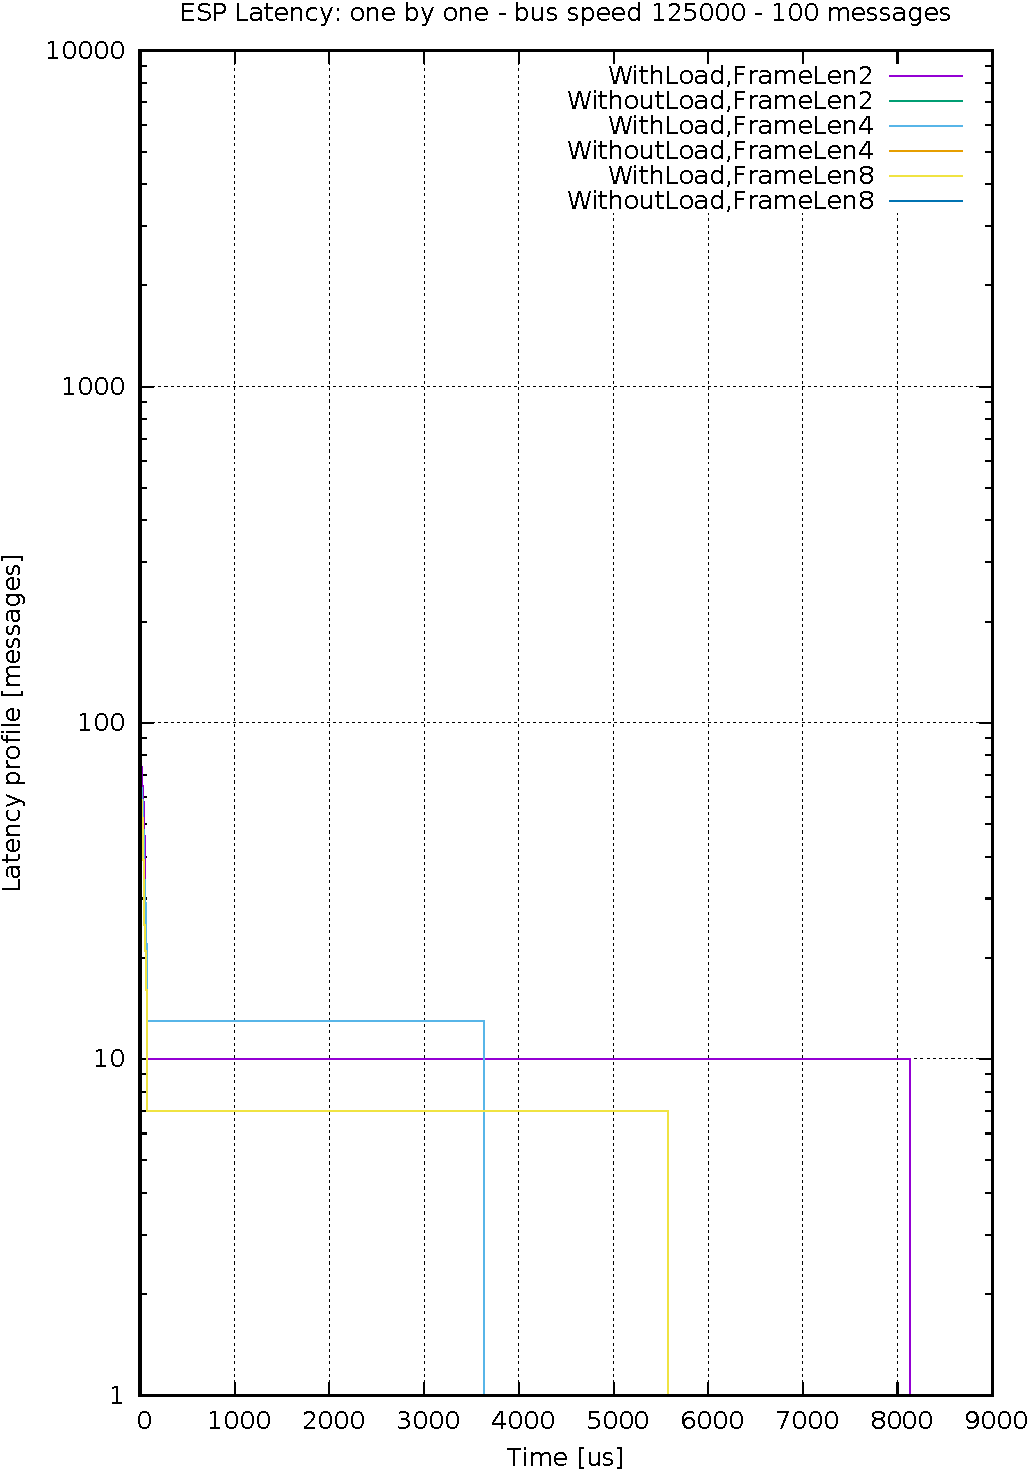
\includegraphics[width=\linewidth]{figures/speed125000_messages100_floodFalse.pdf}
\caption{ESP latency profile: one by one - bus speed 125000 - 100 messages}
\end{figure}

\begin{figure}[htb]
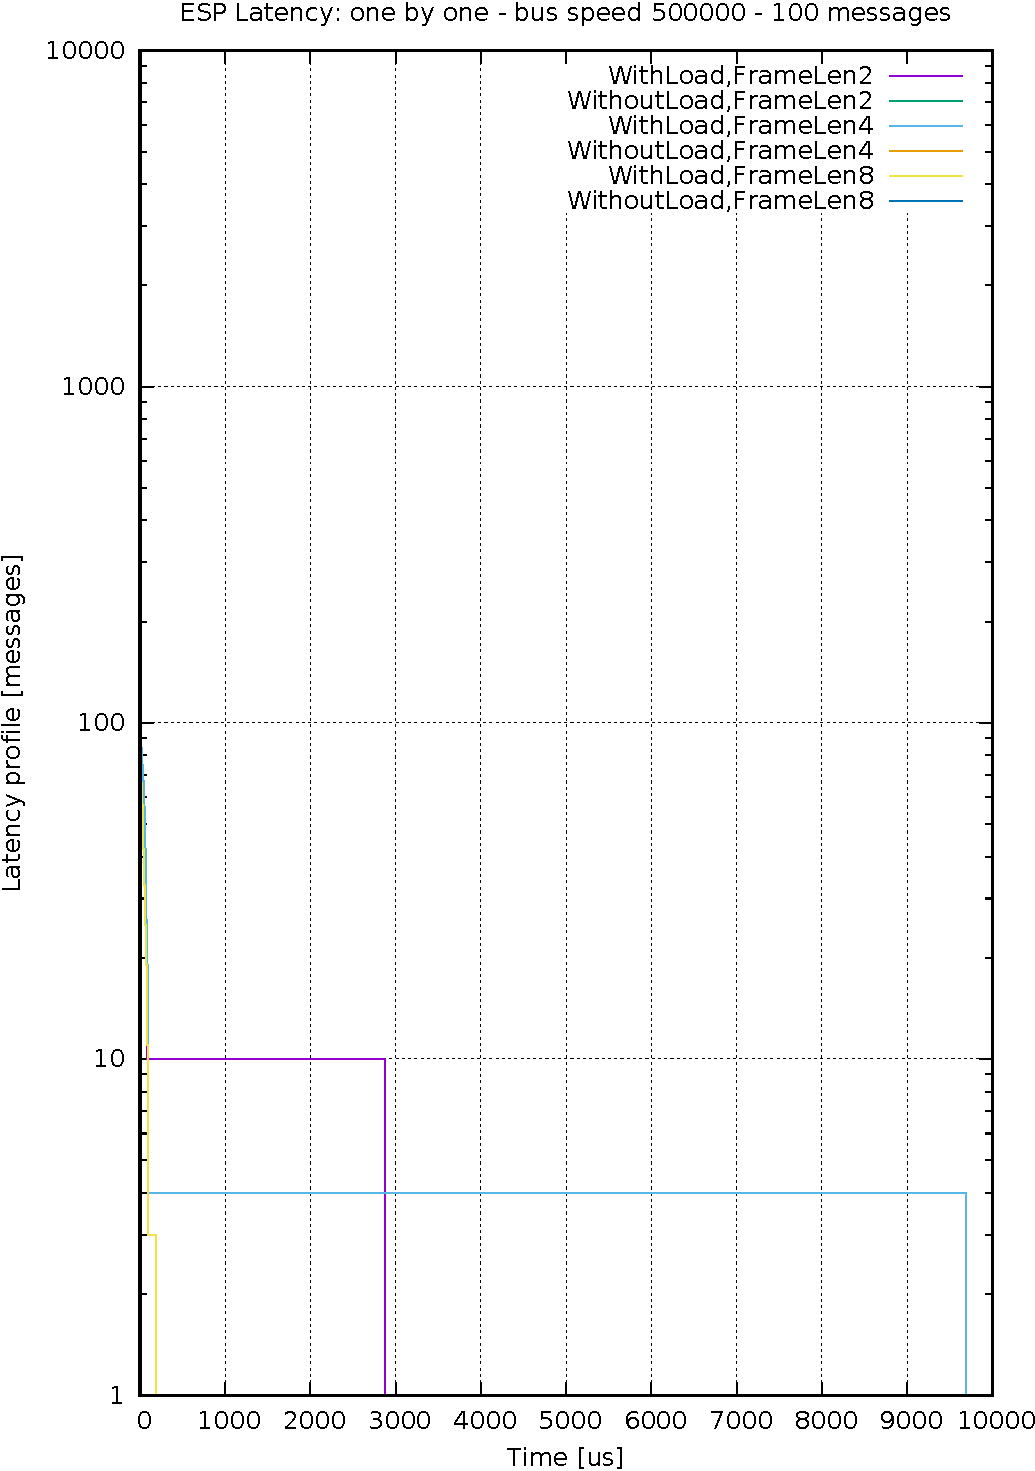
\includegraphics[width=\linewidth]{figures/speed500000_messages100_floodFalse.pdf}
\caption{ESP latency profile: one by one - bus speed 500000 - 100 messages}
\end{figure}

\begin{figure}[htb]
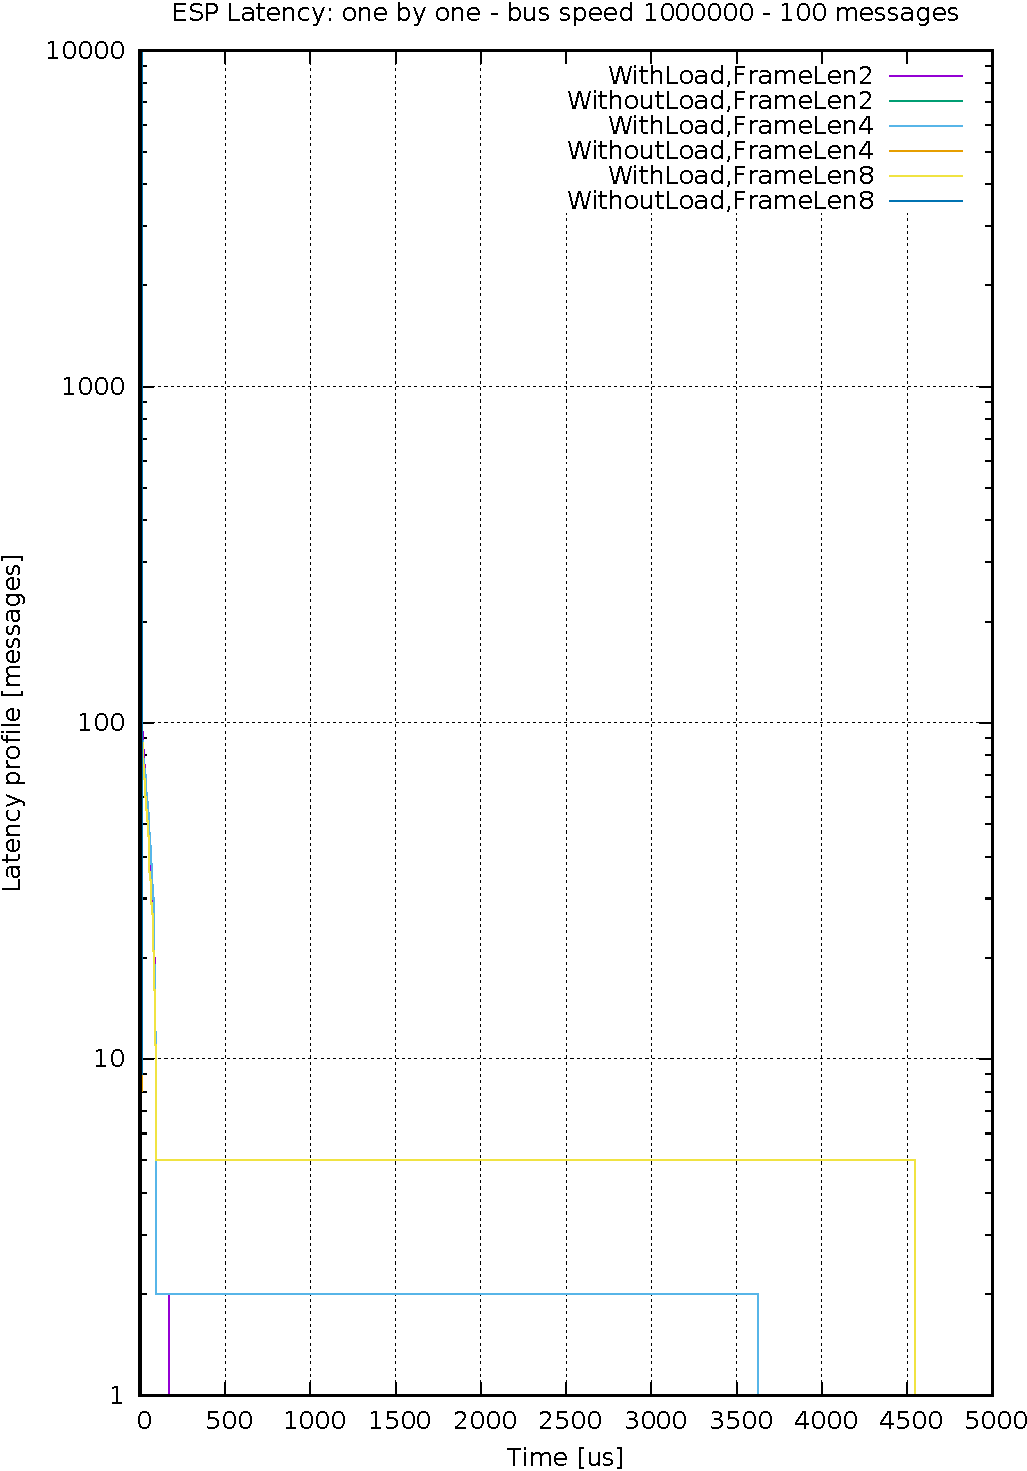
\includegraphics[width=\linewidth]{figures/speed1000000_messages100_floodFalse.pdf}
\caption{ESP latency profile: one by one - bus speed 1000000 - 100 messages}
\end{figure}

\begin{figure}[htb]
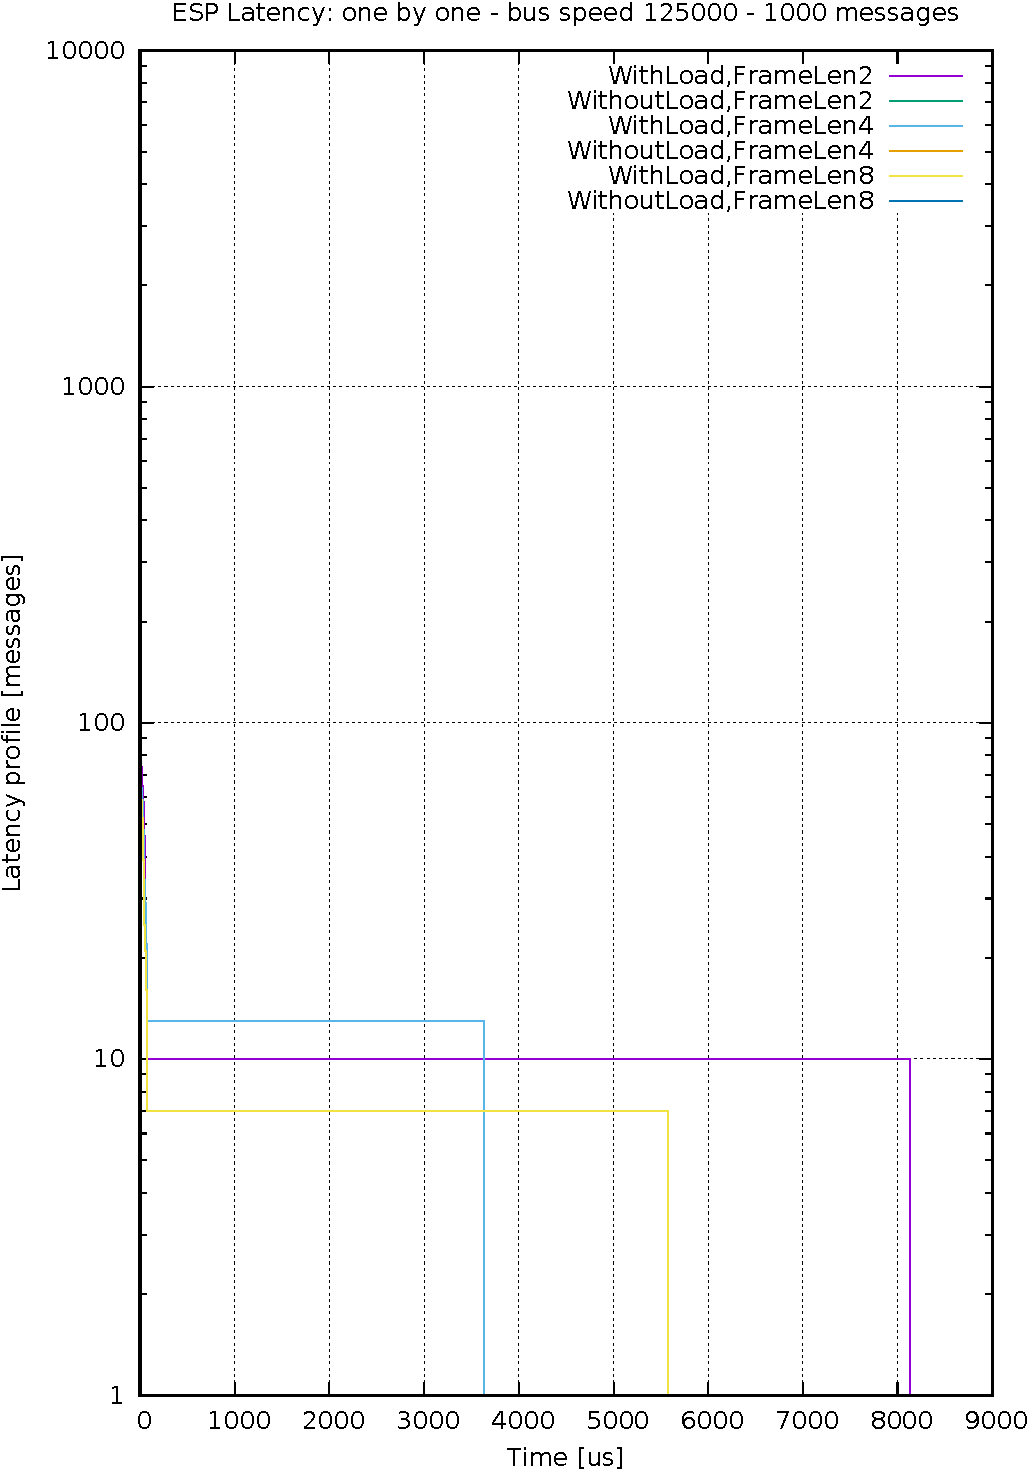
\includegraphics[width=\linewidth]{figures/speed125000_messages1000_floodFalse.pdf}
\caption{ESP latency profile: one by one - bus speed 125000 - 1000 messages}
\end{figure}

\begin{figure}[htb]
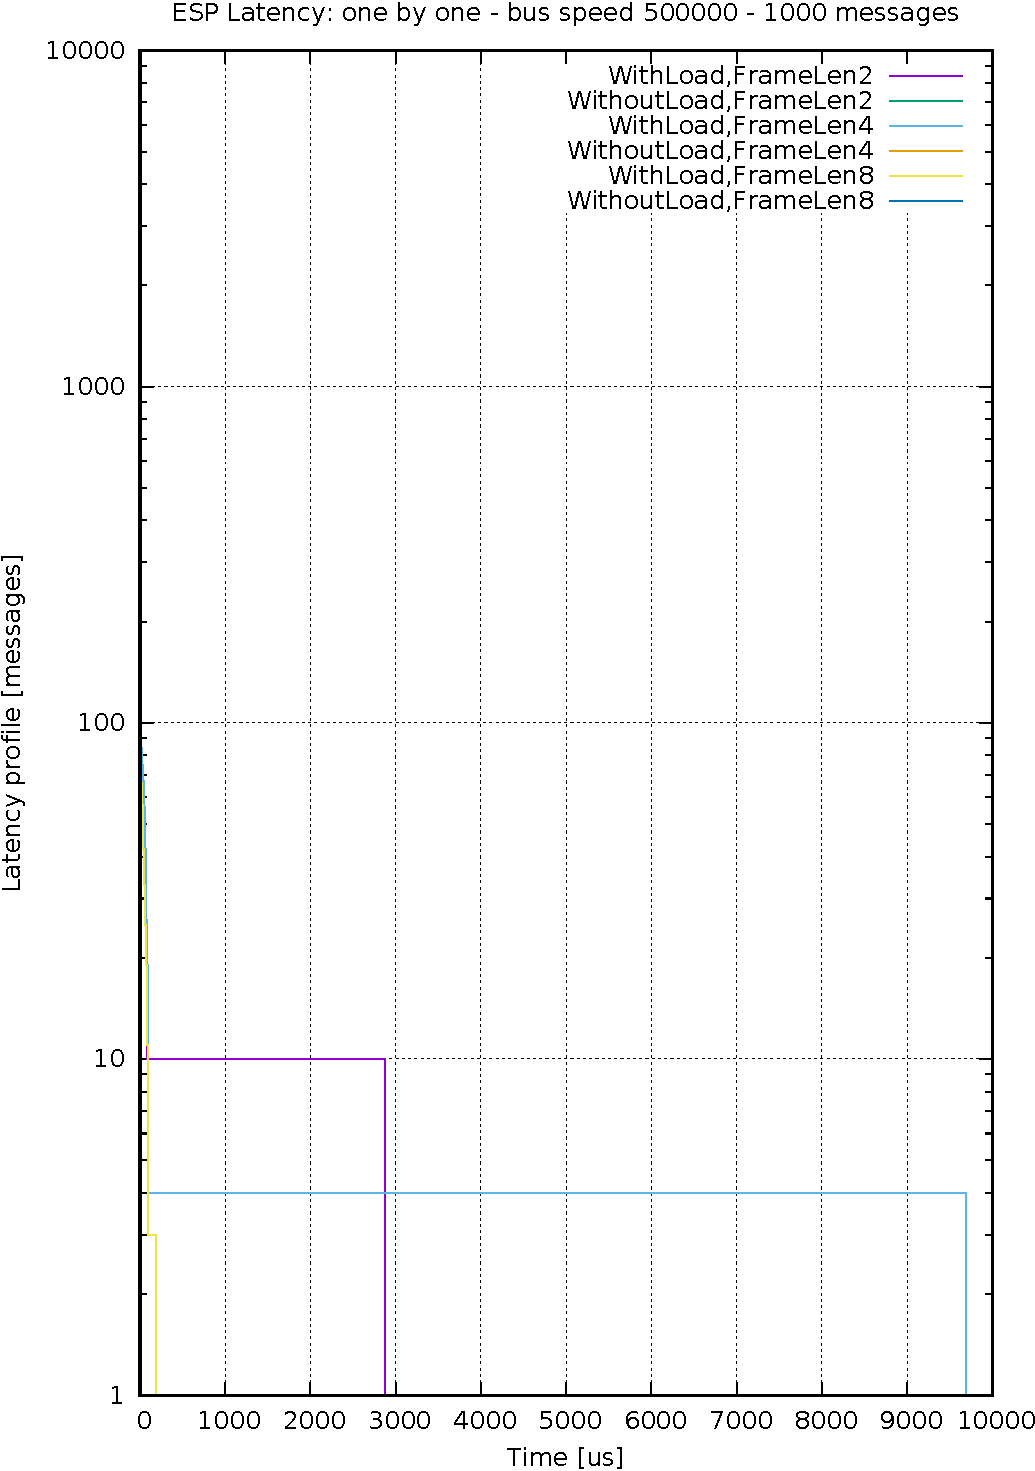
\includegraphics[width=\linewidth]{figures/speed500000_messages1000_floodFalse.pdf}
\caption{ESP latency profile: one by one - bus speed 500000 - 1000 messages}
\end{figure}

\begin{figure}[htb]
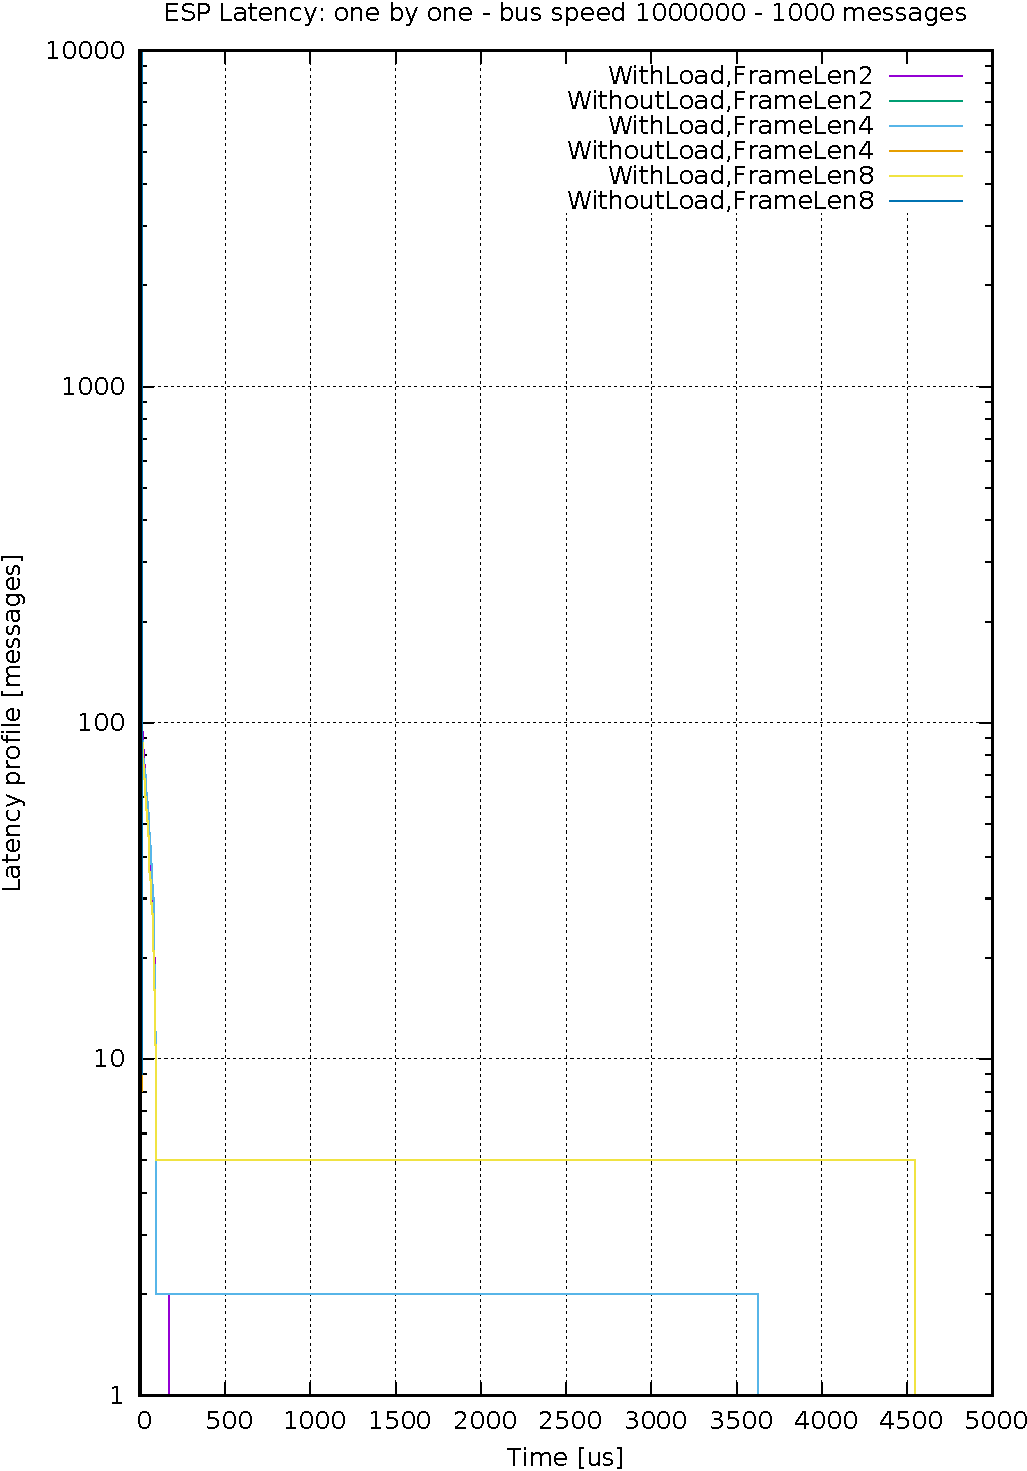
\includegraphics[width=\linewidth]{figures/speed1000000_messages1000_floodFalse.pdf}
\caption{ESP latency profile: one by one - bus speed 1000000 - 1000 messages}
\end{figure}

\begin{figure}[htb]
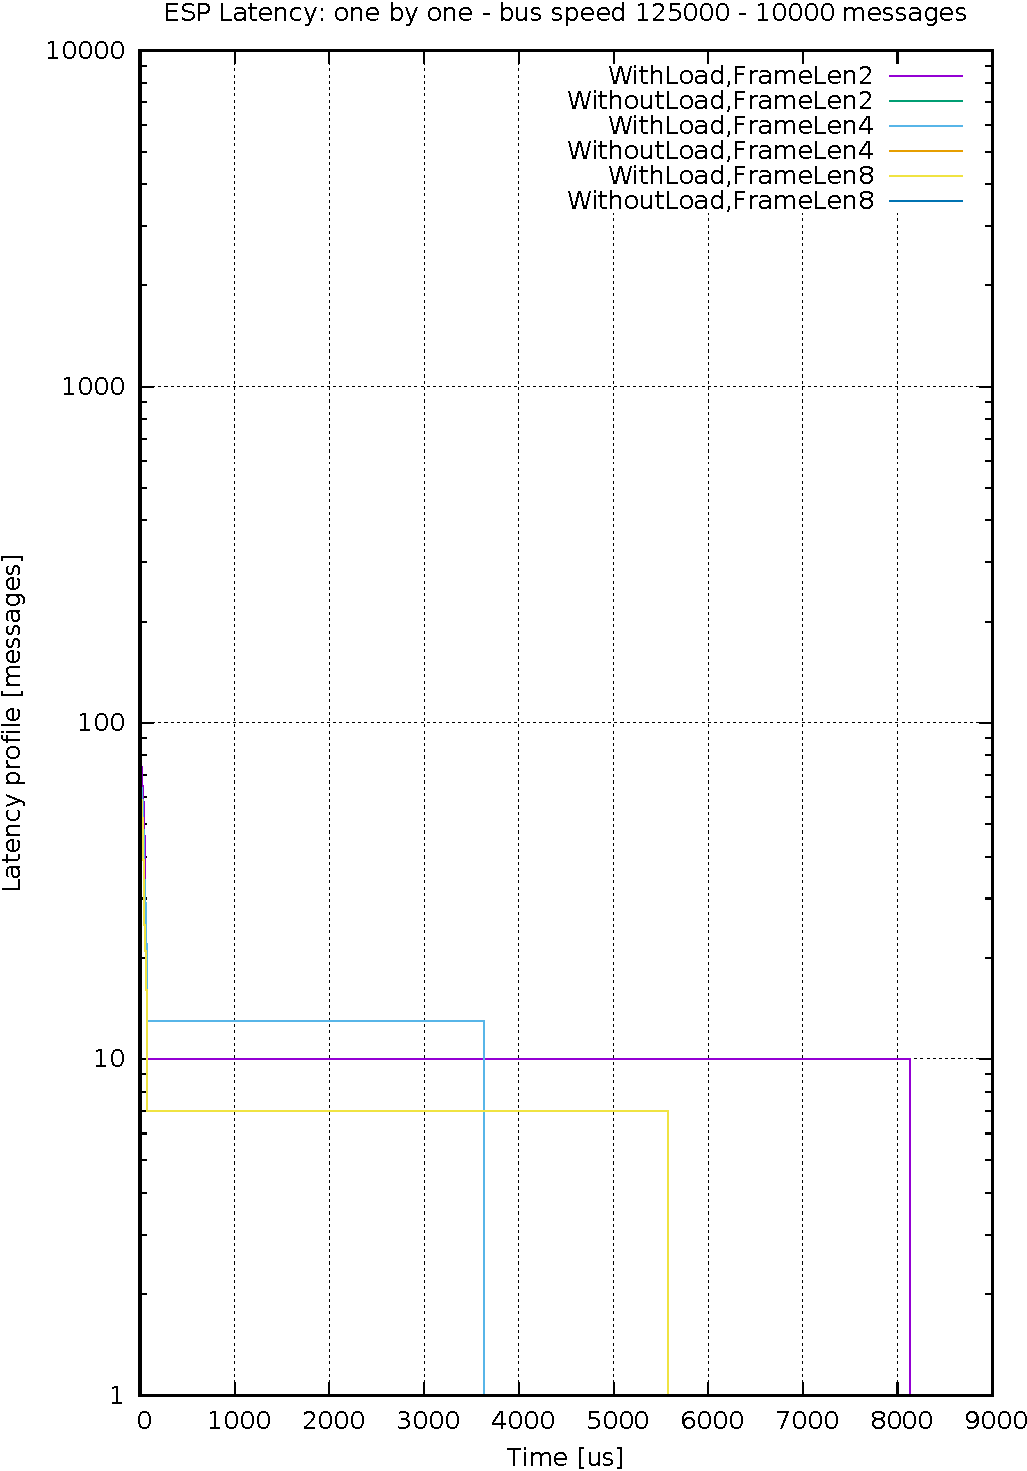
\includegraphics[width=\linewidth]{figures/speed125000_messages10000_floodFalse.pdf}
\caption{ESP latency profile: one by one - bus speed 125000 - 10000 messages}
\end{figure}

\begin{figure}[htb]
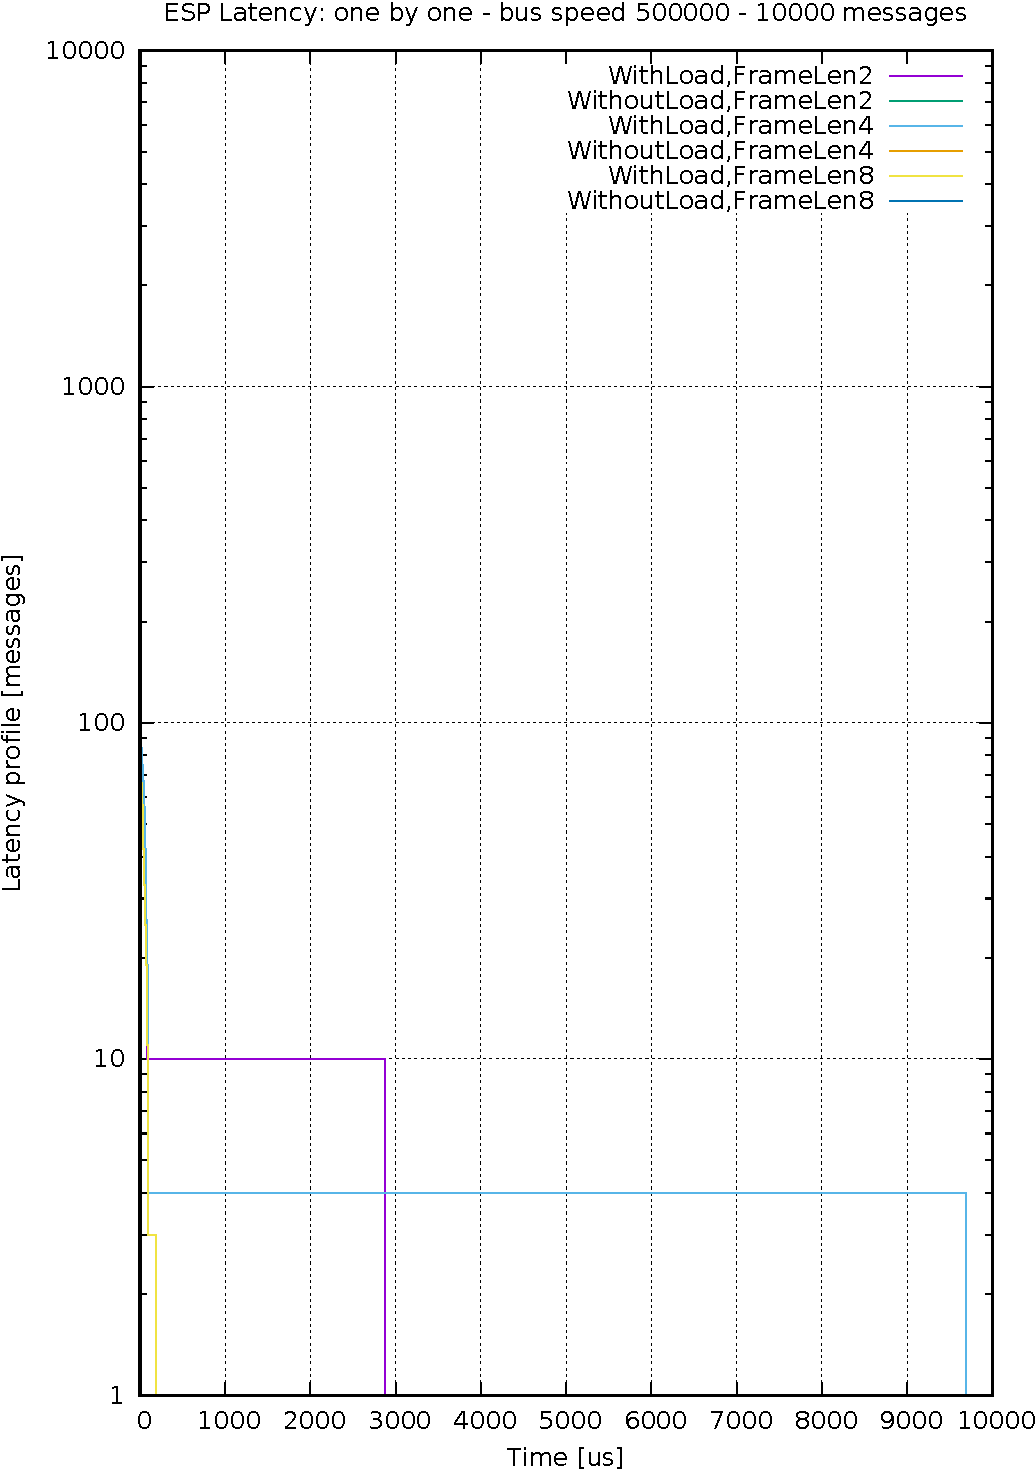
\includegraphics[width=\linewidth]{figures/speed500000_messages10000_floodFalse.pdf}
\caption{ESP latency profile: one by one - bus speed 500000 - 10000 messages}
\end{figure}

\begin{figure}[htb]
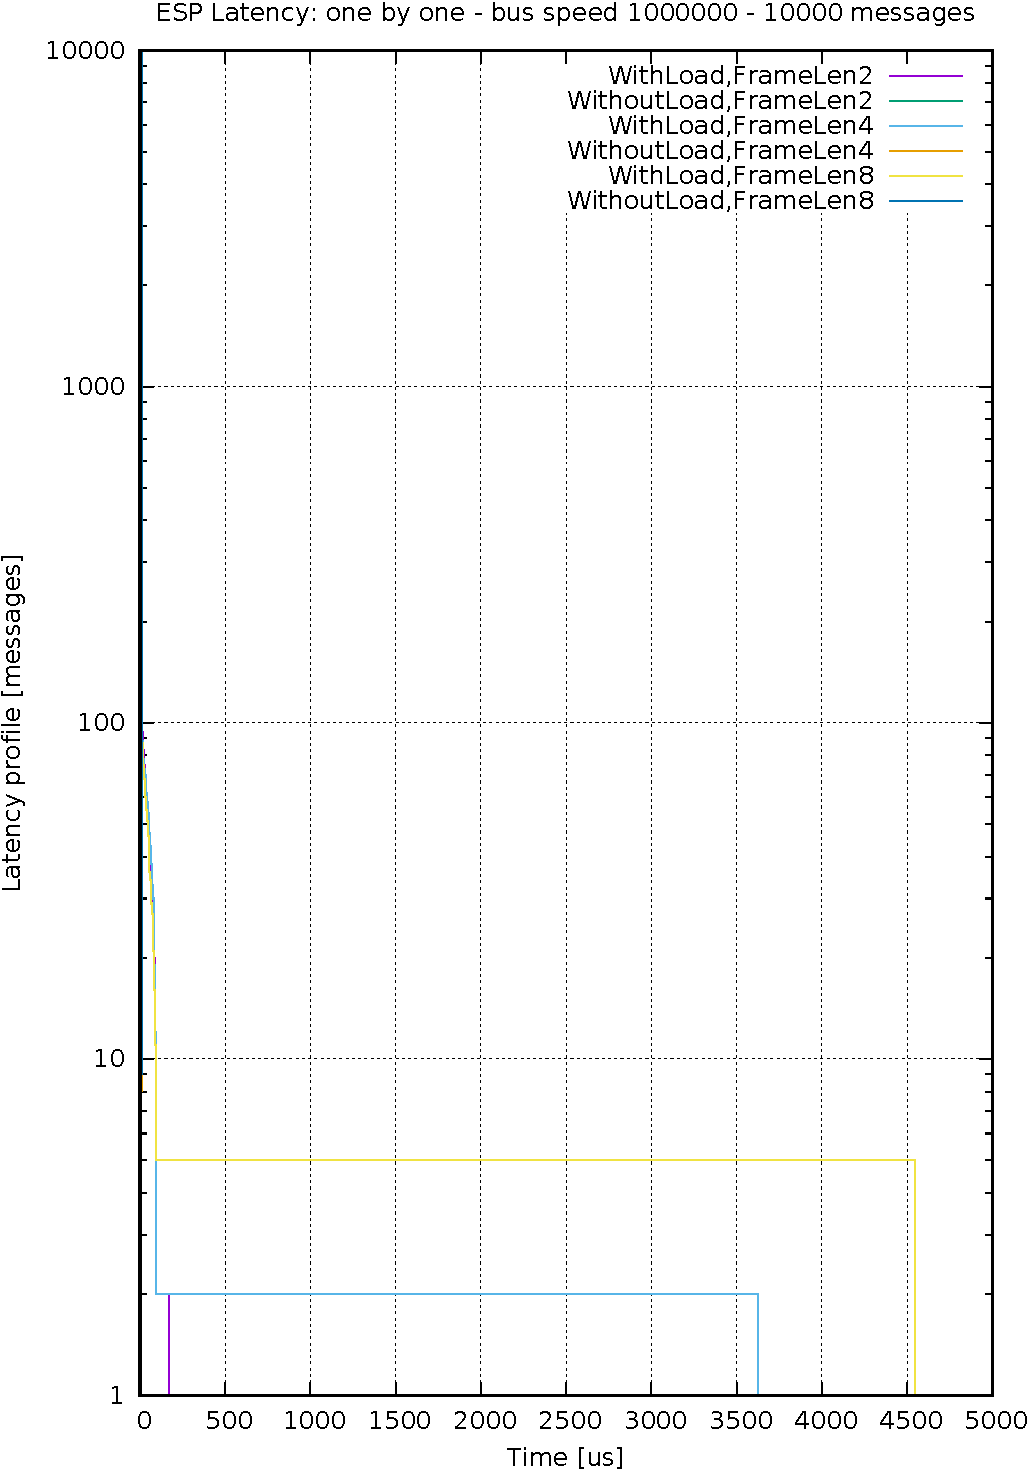
\includegraphics[width=\linewidth]{figures/speed1000000_messages10000_floodFalse.pdf}
\caption{ESP latency profile: one by one - bus speed 1000000 - 10000 messages}
\end{figure}

\end{document}